%!TEX TS-program = xelatex
%!TEX encoding = UTF-8 Unicode

% Load Thesis Class
\documentclass{DEIThesis}

\title{Funzionamento della rete satellitare Starlink}

\author{Matteo Galiazzo}
\studentId{2044941}

% Advisor
\advisor{Prof. Roberto Corvaja}

% If you are co-advised
\coadvisor{}
\coadvisorsUniversity{}

\university{Università di Padova}
\mastername{Ingegneria informatica}
\academicYear{2023/2024}

\begin{filecontents*}[overwrite]{\jobname.xmpdata}
    \Title{Funzionamento della rete satellitare Starlink}
    \Author{Matteo Galiazzo}
    \Language{it-IT}
    \Keywords{Ingegneria informatica\sep LaTeX}
\end{filecontents*}

\usepackage{makecell}
\usepackage{gensymb}
% Document

\begin{document}
    % The front matter (Cover, ToC, Abstract, etc...)
    \frontmatter

    % The main content
    \mainmatter
    
    %!TEX root = ../main.tex

\chapter{Tipi di costellazioni satellitari}
\label{chp:intro}

Una costellazione di Internet via satellite è una costellazione di satelliti artificiali che forniscono servizi di Internet. In particolare, il termine si riferisce a una nuova generazione di costellazioni molto grandi (a volte indicate come megacostellazioni) che orbitano nell'orbita terrestre bassa (LEO) per fornire servizi Internet a bassa latenza e ad alta larghezza di banda (banda larga) \cite{jose_del_rosario_nsr_2018}.
% Nel 2020, il 63\% delle famiglie che vivono in zone rurali del mondo non ha accesso a Internet a causa dei requisiti infrastrutturali dei cavi sotterranei e delle torri di rete. Le costellazioni Internet via satellite offrono una soluzione a basso costo per espandere la copertura \cite{makena_young_low_2022}.
A novembre 2022, poco più del 63\% degli 8 miliardi di persone nel mondo utilizza Inetrnet, lasciando circa 3 miliardi di persone (e potenziali clienti) non connnessi.
Per colmare questo divario digitale, governi e aziende commerciali private stanno investendo in iniziative per costruire Internet a banda larga basata sullo spazio.
Se avranno successo, questi sforzi hanno il potenziale per connettere rapidamente le persone in tutto il mondo e cambiare l'ambiente spaziale stesso.
Diversi paesi stanno lanciando iniziative nazionali per stabilire costellazioni di satelliti in orbita terrestre bassa (\ac{LEO}) e catturare ampie porzioni di un mercato in crescita, liberando ampie risorse private o statali per farlo.

La competizione per fornire servizi a banda larga dai satelliti non è una novità.
Gli anni '90 hanno visto un simile boom commerciale di Internet a banda larga che ha prodotto scarso successo.
Aziende come Teledesic, Celestri, Globalstar e Iridium hanno tutte proposto grandi costellazioni di comunicazioni satellitari (SATCOM) in \ac{LEO}, ma quasi tutte sono finite in bancarotta all'inizio degli anni 2000.

Oggi la barriera all'ingresso in orbita è notevolmente diminuita poichè la tecnologia, i materiali e le capacità di lancio sono diventati più economici e più ampiamente disponibili.
La concorrenza internazionale per costruire, langiare e gestire un sistema a basso costo e bassa latenza che si estenda in tutto il mondo è feroce, poichè la domanda di servizi internet veloci e affidabili continua a crescere.

A partire dal 2022, solo un operatore, Starlink, fornisce un servizio basato su \ac{LEO} sul mercato libero.
Si stima che il mercato globale SATCOM crescerà fino a 40 miliardi di dollari entro il 2030, in gran parte guidato da iniziative basate su \ac{LEO}.

L'istituzione di una costellazione \ac{LEO}, comporta un investimento iniziale sostanziale, un know-how tecnico specializzato e la capacità di orientarsi in un panorama normativo complesso.
Con l'intensificarsi della concorrenza internazionale nelle comunicazioni \ac{LEO}, è fondamentale che il governo degli stati uniti crei un ambiente normativo abilitante (ma robusto) affinchè le imprese con sede negli Stati Uniti possano prosperare in patria e all'estero.

Il più grande concorrente degli Stati Uniti nella corsa alla connettività globale tramite banda larga satellitare è la Cina.
La Cina ha proposto una costellazione di 13000 satelliti in \ac{LEO} per soddisfare le esigenze residenziali e aziendali nel mercato cinese, nonchè nei mercati Internet sottosviluppati in tutto il mondo \cite{makena_young_low_2022}.

\section{Vantaggi della Low Earth Orbit}

I satelliti sono tipicamente lanciati in una di tre orbite: Low Earth Orbit (LEO) dai 160 ai 2'000 km, Medium Earth Orbit (MEO) dai 2000 ai 35786 km, o Geosynchronous Orbit (GEO) a 42164 km.
Ciascuna delle tre orbite ha i suoi vantaggi.
Per esempio, una costellazione in GEO può avere copertura globale con solo tre satelliti per la sua distanza dalla superficie terrestre.
La GEO è popolare per le comunicazioni per questo motivo.
Però, dato che i satelliti sono così distanti dalla Terra la latenza è molto alta.

\begin{figure}[htbp]
  \centering
  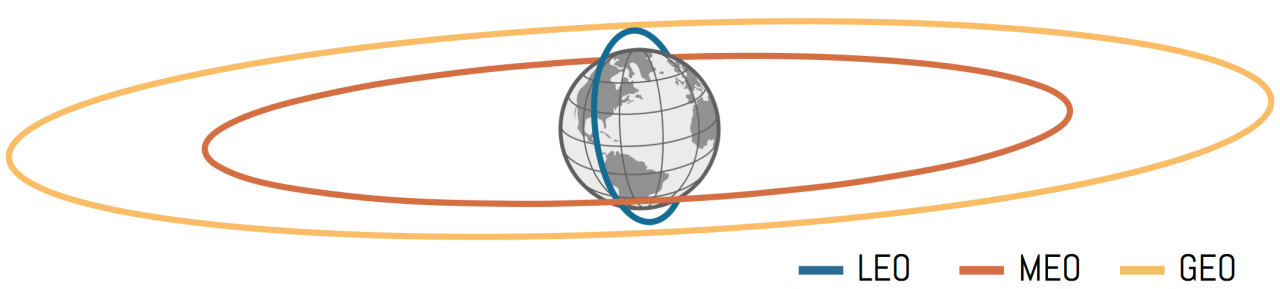
\includegraphics[width=0.9\linewidth]{./res/img/leo_orbit.png}
  \caption{Orbite terrestri di popolare utilizzo \cite{thomas_g_roberts_popular_2022}}
  \label{fig:leo-orbit}
\end{figure}

Le nuove generazioni di internet via satellite stanno collocando i satelliti in \ac{LEO} invece della tradizionale \ac{GEO} per una serie di motivi.
Infatti i satelliti lanciati in \ac{LEO} sono tipicamente più piccoli e più leggeri di quelli in \ac{GEO}, quindi serve meno carburante per mandarli in orbita e in generale sono ridotti i costi di lancio.
Inoltre, dato che i satelliti sono più vicini i terminali utente possono rilevare più satelliti allo stesso tempo e conettersi quindi al satellite più conveniente.

Le comunicazioni dalla \ac{LEO} hanno anche una latenza inferiore rispetto ai satelliti in \ac{GEO} perchè sono molto più vicini alla superficie terrestre.
Gli operatori satellitari \ac{LEO} sostengono che una pagina web può essere aperta circa otto volte più velocemente quando si utilizzano i satelliti \ac{LEO} rispetto a quando si utilizza un sistema SATCOM tradizionale in \ac{GEO}, qualcosa che è diventato più importante per i consumatori che vogliono interagire online quasi in tempo reale.
Ciò significa che Internet satellitare deve essere in grado di supportare applicazioni ad alta velocità come streaming, videoconferenza e giochi in tempo reale \cite{makena_young_low_2022}.

% https://en.wikipedia.org/wiki/SpaceX#Starlink_2
\section{Starlink}

Starlink è una costellazione internet via satellite operata da Starlink Services LLC, una consociata interamente controlla dalla società aerospaziale americana SpaceX, che fornisce copertura a oltre 100 paesi e territori.
Mira inoltre a firnire la banda larga mobile a livello mondiale.

SpaceX ha iniziato a lanciare i satelliti Starlink nel 2019.
A partire da settembre 2024, la costellazione è composta da oltre 7000 piccoli satelliti prodotti in serie in orbita terrestre bassa (\ac{LEO}) che comunicano con terminali utente sulla Terra \cite{jonathan_mcdowell_starlink_nodate}.
SpaceX prevede di schierare quasi 12000 satelliti, con una prossibile estensione successiva a 34400.
SpaceX ha annunciato di aver raggiunto più di 1 milione di abbonati nel dicembre 2022 e 4 milioni di abbonati nel settembre 2024 \cite{starlink_starlink_nodate}.

Nel maggio 2018, SpaceX ha stimato che il costo totale della progettazione, costruzione e dispiegamento della costellazione sarebbe stato di almeno 10 milardi di dollari \cite{michael_baylor_block_2018}.
Secondo quanto riferito, i ricavi di Starlink nel 2022 sono stati di 1.4 milardi di dollari, accompagnati da una perdita netta, con un piccolo profitto iniziato solo nel 2023.
Si prevede che i ricevi raggiungeranno i 6.6 milardi di dollari nel 2024 \cite{eric_berger_analyst_2024}.

Gli astronomi hanno espresso preoccupazione sull'effetto che la costellazione potrebbe avere sull'astronomia da terra e su come i satelliti contribuiranno a un ambiente orbitale già congestionato.
SpaceX ha tentato di mitigare i problemi di interferenza astronomica con misure per ridurre la luminosità dei satelliti durante il funzionamento.
I satelliti sono dotati di propulsori ad effetto Hall che consentono loro di alzare l'orbita, mantenere una posizione di stazionamento e uscire dall'orbita alla fine della loro vita.
Sono inoltre progettati per evitare collisioni in modo autonomo e senza intoppi sulla base dei dati di tracciamento collegati in uplink \cite{spacex_astronomy_2020}.
    %!TEX root = ../main.tex

\chapter{Architettura del sistema}

Chiariamo come prima cosa la differenza tra un antenna per la televisione satellitare e un'antenna Starlink.
Le parabole TV utilizzano un riflettitore parabolico per focalizzare le onde elettromagnetiche che costituiscono i segnali televisivi inviati dai satelliti di trasmissione in orbita attorno alla terra e un'altitudine di 35'000 km.
Le parabole TV ricevono solo segnali televisivi dallo spazio, non possono inviare dati.
La parabola Starlink, invece, invia e riceve dati Internet da un satellite starlink in orbita a 550km di distanza.
I fasci tra la parabola Starlink e il satellite deovno essere concentrati in fasci potenti e stretti, continuamente orientati per puntare l'uno verso l'altro \cite{branch_education_how_2022}.
Attualmente ci sono 6398 satelliti Starlink in orbita \cite{jonathan_mcdowell_starlink_nodate}.

\begin{figure}[ht]
  \centering
  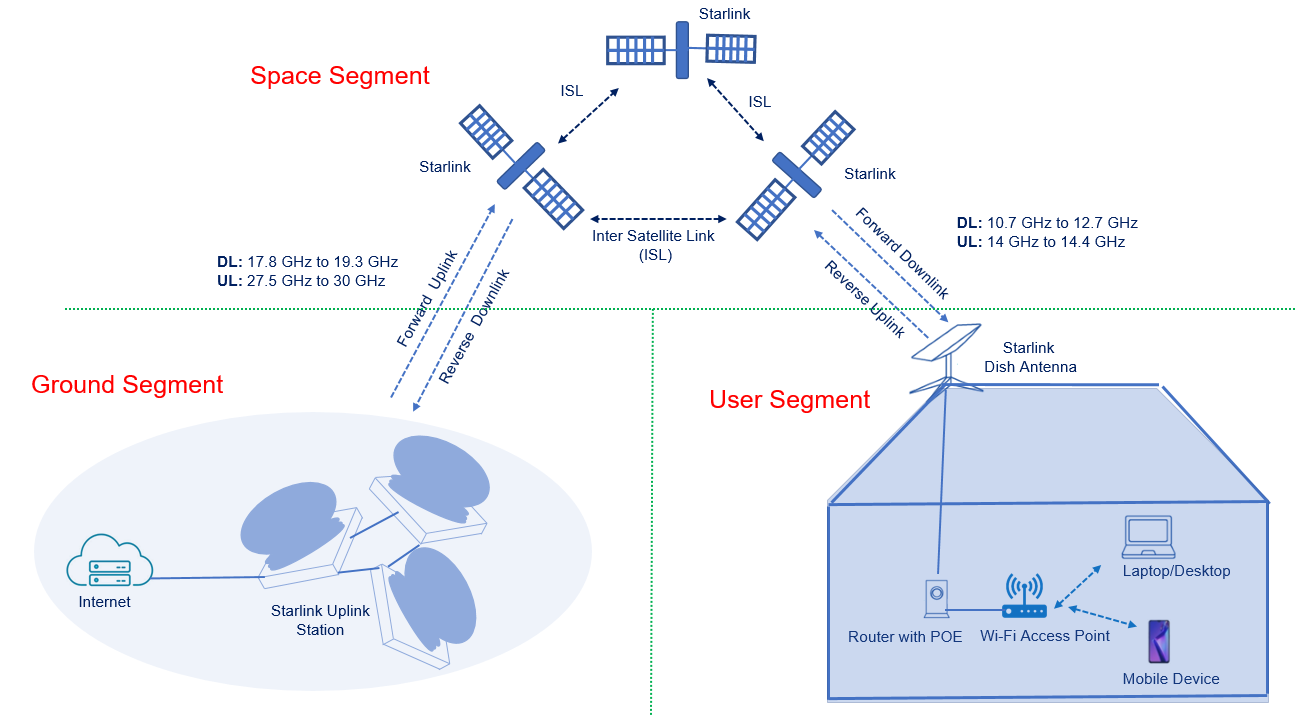
\includegraphics[width=0.9\linewidth]{./res/img/starlink-system-architecture.png}
  \caption{Architettura di sistema \cite{techplayon_spacex_2024}}
  \label{fig:starlink-system-architecture}
\end{figure}

\section{Segmento spaziale}
Questo segmento è costituito da un numero di satelliti in \ac{LEO}. Si tratta di piccoli satelliti a basso costo che pesano circa 260kg (nella versione 1.0), operano in \ac{Ku} e \ac{Ka} band e hanno durata di vita di 5-7 anni. \cite{techplayon_spacex_2024} Questi satelliti collegano l'utente a Internet.

Poichè esiste un numero enorme di satelliti questi comunicano tra loro attraverso \ac{ISL}.
% LEGGERE PAPER ISL OTTICO

\section{Segmento di terra}
I segmenti di terra includono diverse facilities che gestiscono la rete e forniscono connettività internet ai satelliti. Questi funzionano anche da Graund Station e sono localizzati strategicamente intorno al mondo per fornire copertura a zone remote e con poca connettività a internet.
La ground station è connessa all'\ac{ISP} tramite fibra.

\section{Segmento utente}
Il segmento utente comprende l'area in cui le persone utilizzano i servizi internet tramite il kit che viene fornito e che comprende l'antenna per la trasmissione, il cavo di alimentazione, il router (tranne nella versione mini dell'antenna dove il router è integrato all'antenna) e il cavo di rete per connettere l'antenna al router se quest'ultimo è incluso.

\subsection{Antenna}

\subsubsection{Struttura generale}
Aprendo la parabola (versione 1.0 revisione 2) troviamo sul retro una coppia di motori e un cavo ethernet che si collega al router.
Questi motori non muovono continuamente la parabola per puntare direttamente al satellite con cui comunica; vengono utilizzati solo durante la configurazione iniziale per orientare l'antenna nella direzione generale corretta.
Aprendo la parabola troviamo una piastra posteriore strutturale in alluminio e, dall'altro lato, una grande scheda a circuiti stampati (PCB). Su un lato ci sono 640 microchip piccoli e 20 microchip più grandi, disposti in un pattern con tracce che si diramano dai microchip più grandi a quelli più piccoli, insieme a chp aggiuntivi, inclusa la CPU principale e il modulo GPS sul bordo del PCB. Sull'altro lato cisono circa 1'400 cerchi di rame con una griglia di quadrati tra i cerchi.
Nel livello successivo c'è uno schema a nido d'ape in gomma con piccoli cerchi di rame intagliati e dietro troviamo un altro schema a nido d'ape e poi la copertura anteriore della parabola.
Abbiamo quindi 1280 antenne disposte in un pattern esagonale a nido d'ape, con ciascuna pila di cerchi di rame che rappresenta una singola antenna controllata dai microchip sul PCB.
Questo enorme array funziona insieme in quella che è chiamata un'antenna phased array per inviare e ricevere onde elettromagnetiche che vengono direzionate verso e da un satellite Starlink in orbita a 550km di distanza.

\subsubsection{Funzionamento dell'antenna Aperture Couple Patch}

\begin{figure}[htbp]
  \centering
  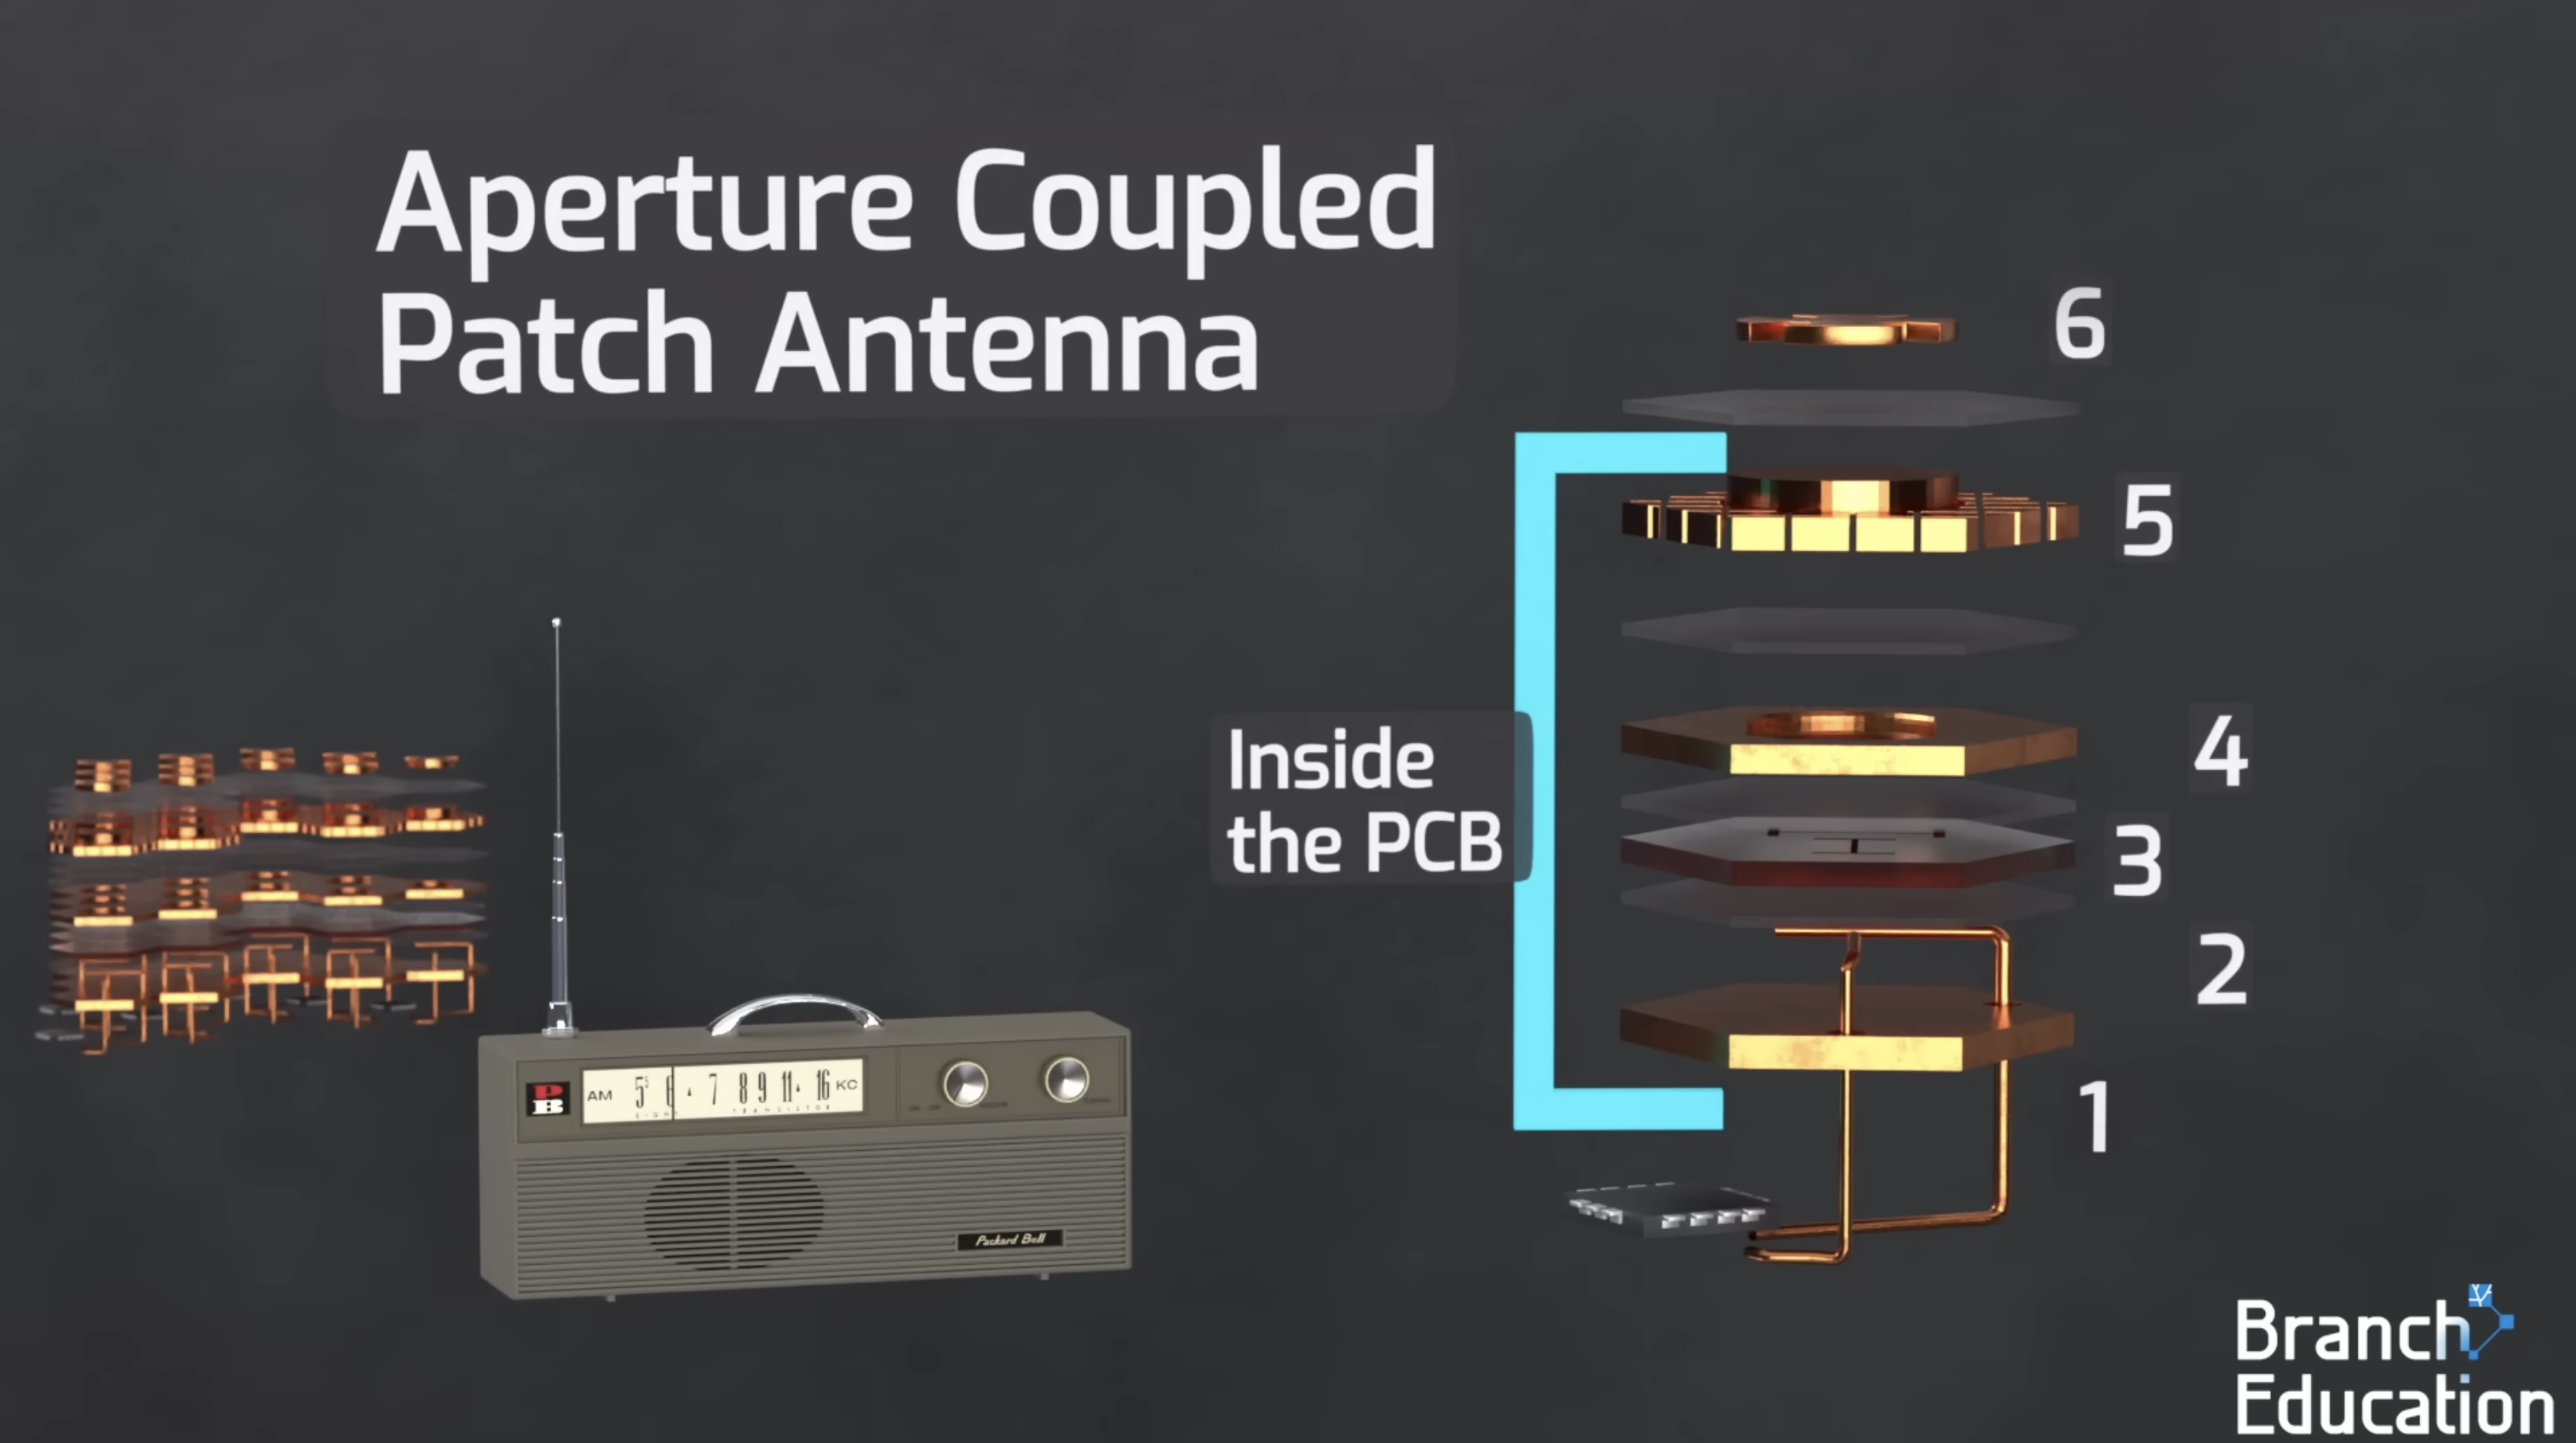
\includegraphics[width=0.8\linewidth]{./res/img/antenna_pcb.png}
  \caption{Aperture Couple Patch antenna \cite{branch_education_how_2022}}
  \label{fig:aperture-couple-patch-antenna}
\end{figure}

Nella figura \ref{fig:aperture-couple-patch-antenna} possiamo vedere un'aperture couple patch antenna, composta di 6 layer, il più dei quali all'interno del PCB.
Per semplificare la sua compressione semplifichiamola rimuovendo per il momento alcuni layer per semplificare la sua comprensione, e vediamo i principi base di come si genera un'onda elettromagnetica che si propaga da quest'antenna.

Per iniziare, sul fondo abbiamo una micro linea di trasmissione elettrica che arriva da uno dei piccoli microchip.
Questa linea di trasmissione è solo un filo di rame che termina sotto la pila dell'antenna.
Mandiamo una tensione sinusodiale alla frequenza di 12 GHz al filo di alimentazione, che vuol dire che il segnale passa da positivo a negativo ogni 83 pico secondi.
Al di sopra del filo di rame di alimentazione abbiamo un cerchio di rame con intagli chiamato patch d'antenna.

Con la corrente continua o alternata a bassa frequenza, non succederebbe molto perchè il patch è isolato, ma con un segnale ad alta frequenza la potenza inviata al filo di alimentazione viene accoppiata o inviata al patch.
Questo fenomeno avviene perchè quando la tensione è al fondo della sua sinusoide, o al minimo, c'è una concentrazione di elettroni spinti verso l'estremità del filo di alimentazione, creando così una zona di carica negativa che corrisponde alla massima tensione negativa.
Questa concentrazione di elettroni sulla punta del filo respinge tutti gli elettroni, compresi quelli sulla parte superiore del patch, e di conseguenza questi elettroni vengono spinti verso l'altro lato del patch circolare.
In questo modo, un lato del patch diventa carico positivamente, mentre l'altro diventa carico negativamente, creando così campi elettrici tra il patch e il filo di alimentazione.
Tuttavia, quando invertiamo la tensione al filo di rame 42 picosecondi dopo, abbiamo una concentrazione di cariche positive, o una mancanza di elettroni all'estremità del filo, e quindi gli elettroni nel patch fluiscono verso l'altro lato, la tensione nel patch è invertita e anche la direzione dei campi elettrici è invertita.

\begin{figure}[htbp]
  \centering
  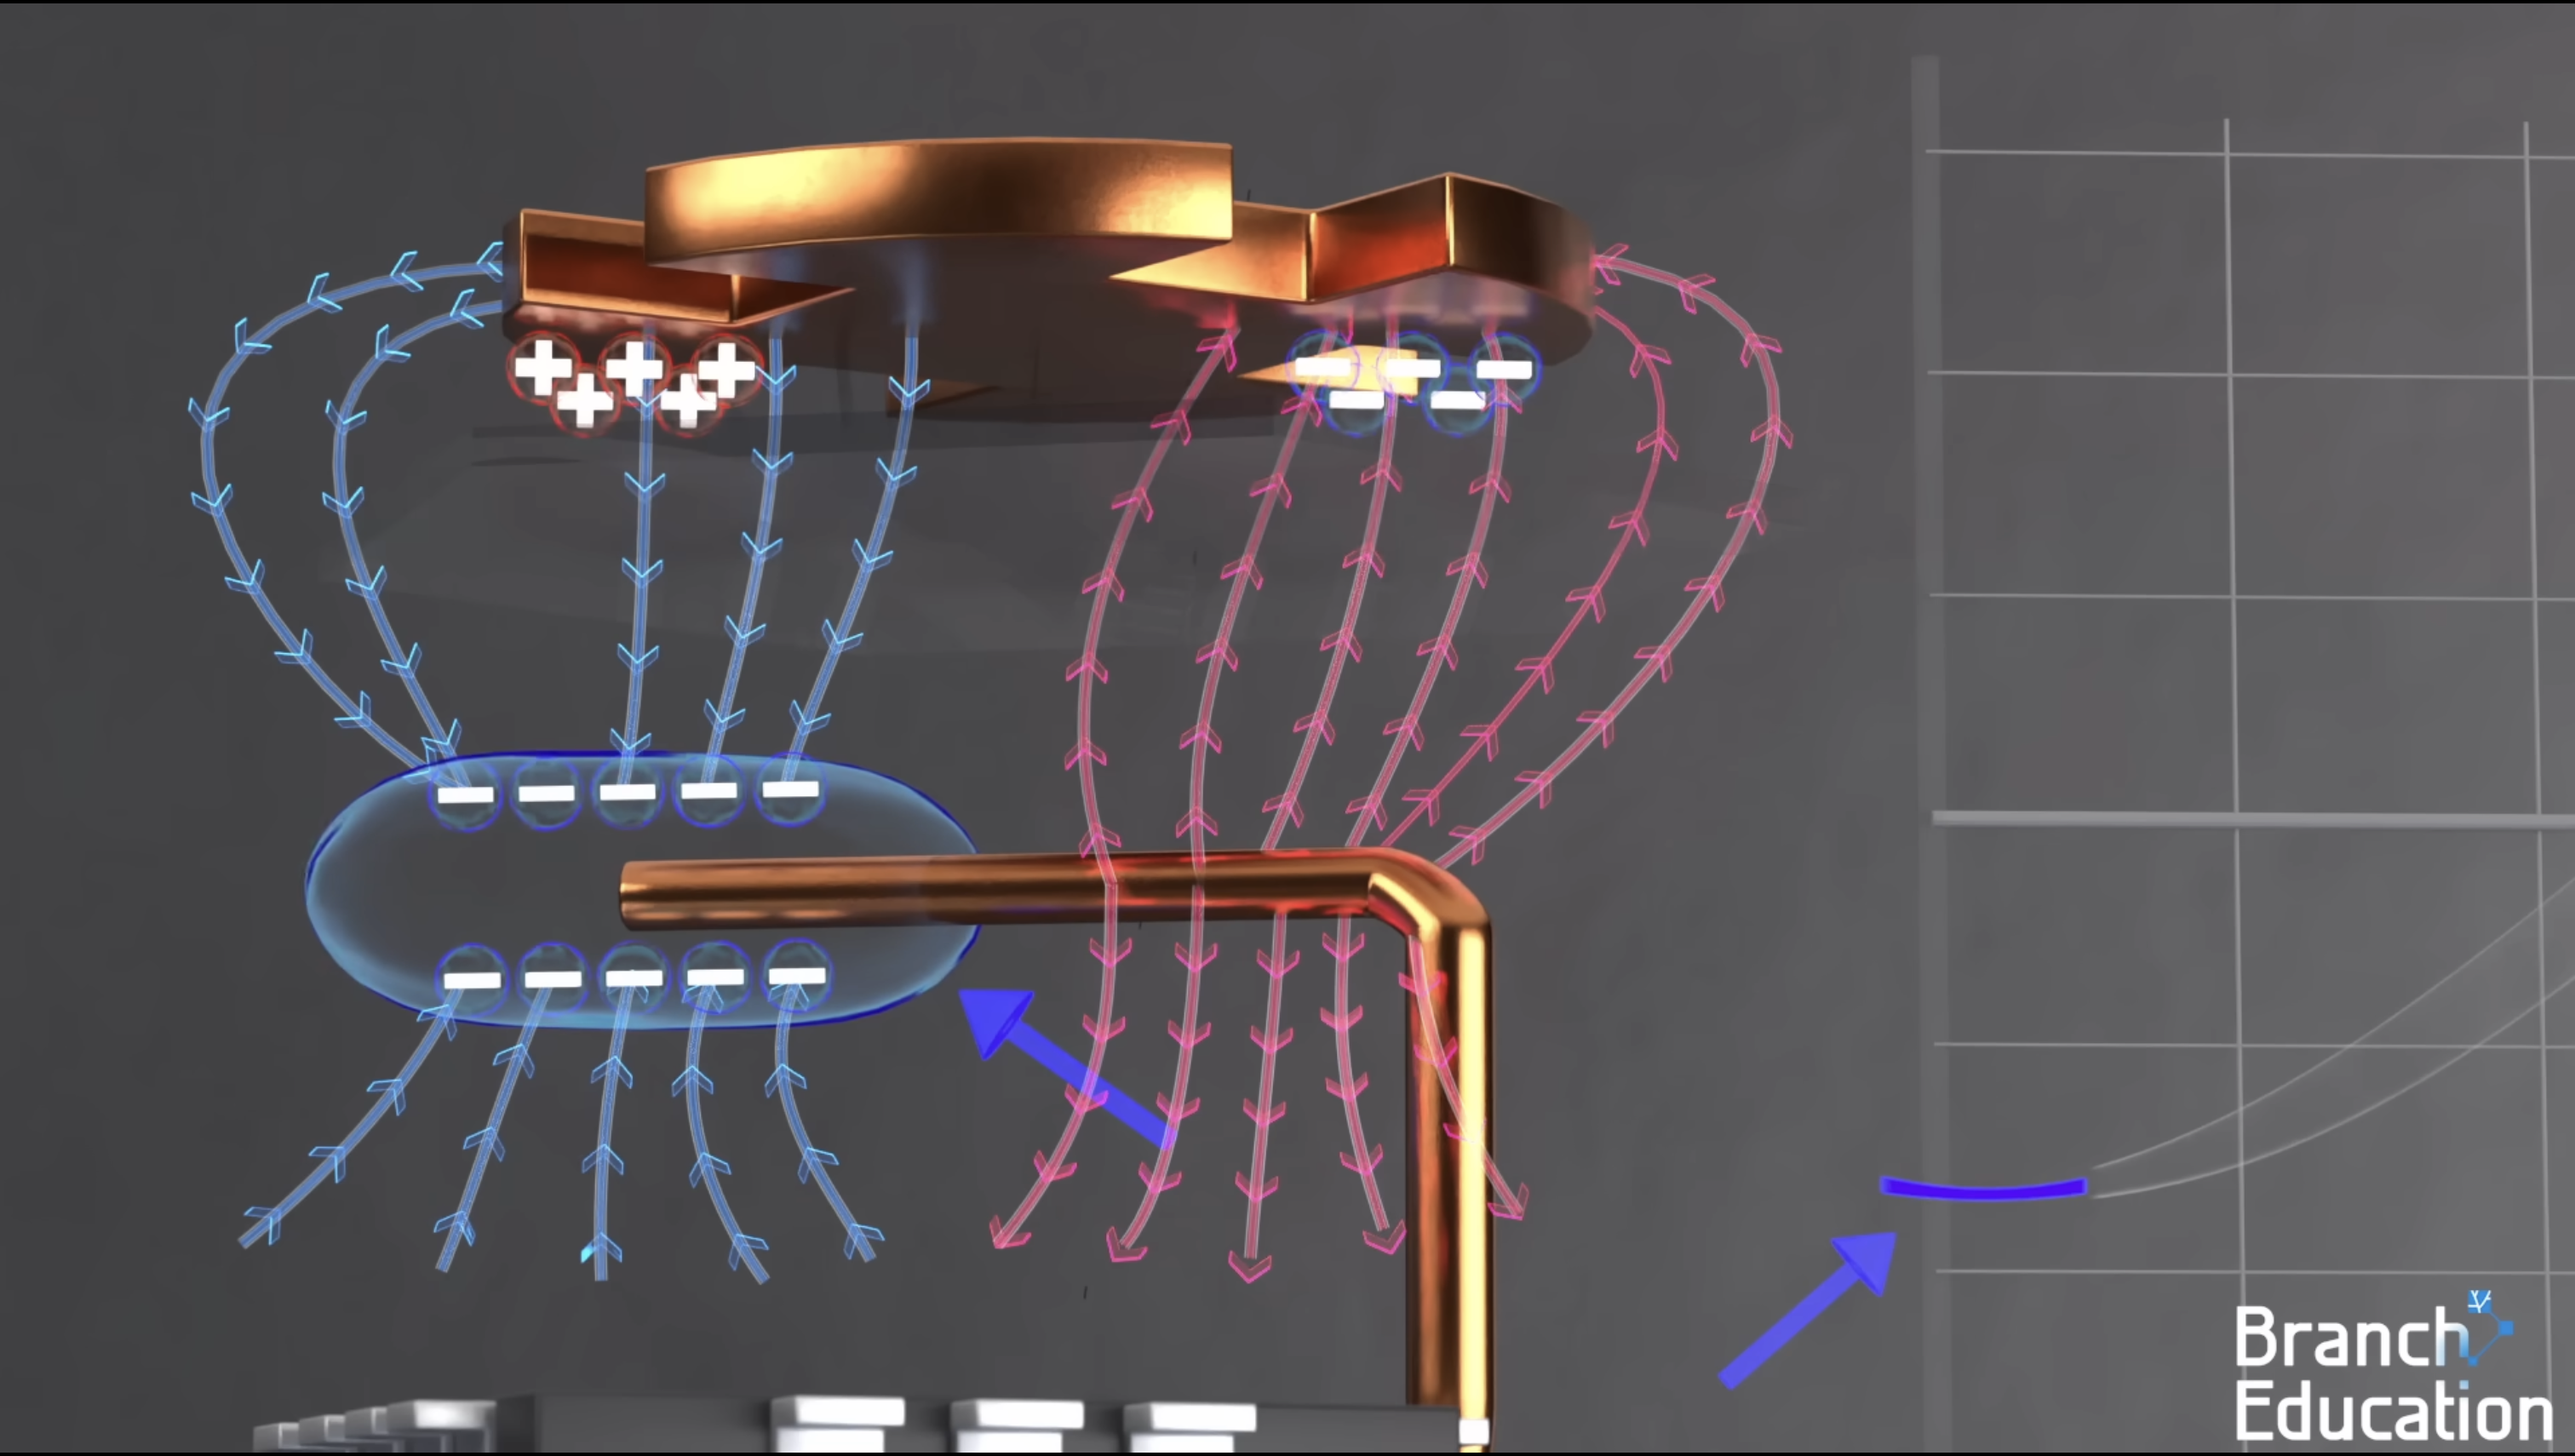
\includegraphics[width=0.8\linewidth]{./res/img/antenna_voltage_applied.png}
  \caption{Aperture Couple Patch antenna con un segnale applicato \cite{branch_education_how_2022}}
  \label{fig:aperture-couple-patch-antenna-voltage-applied}
\end{figure}

Poiché la tensione del filo di alimentazione oscilla con un intervallo di 42 picosecondi tra un picco e un avvallamento, anche i campi elettrici nel patch oscilleranno mentre gli elettroni vanno avanti e indietro.

\begin{figure}[htbp]
  \centering
  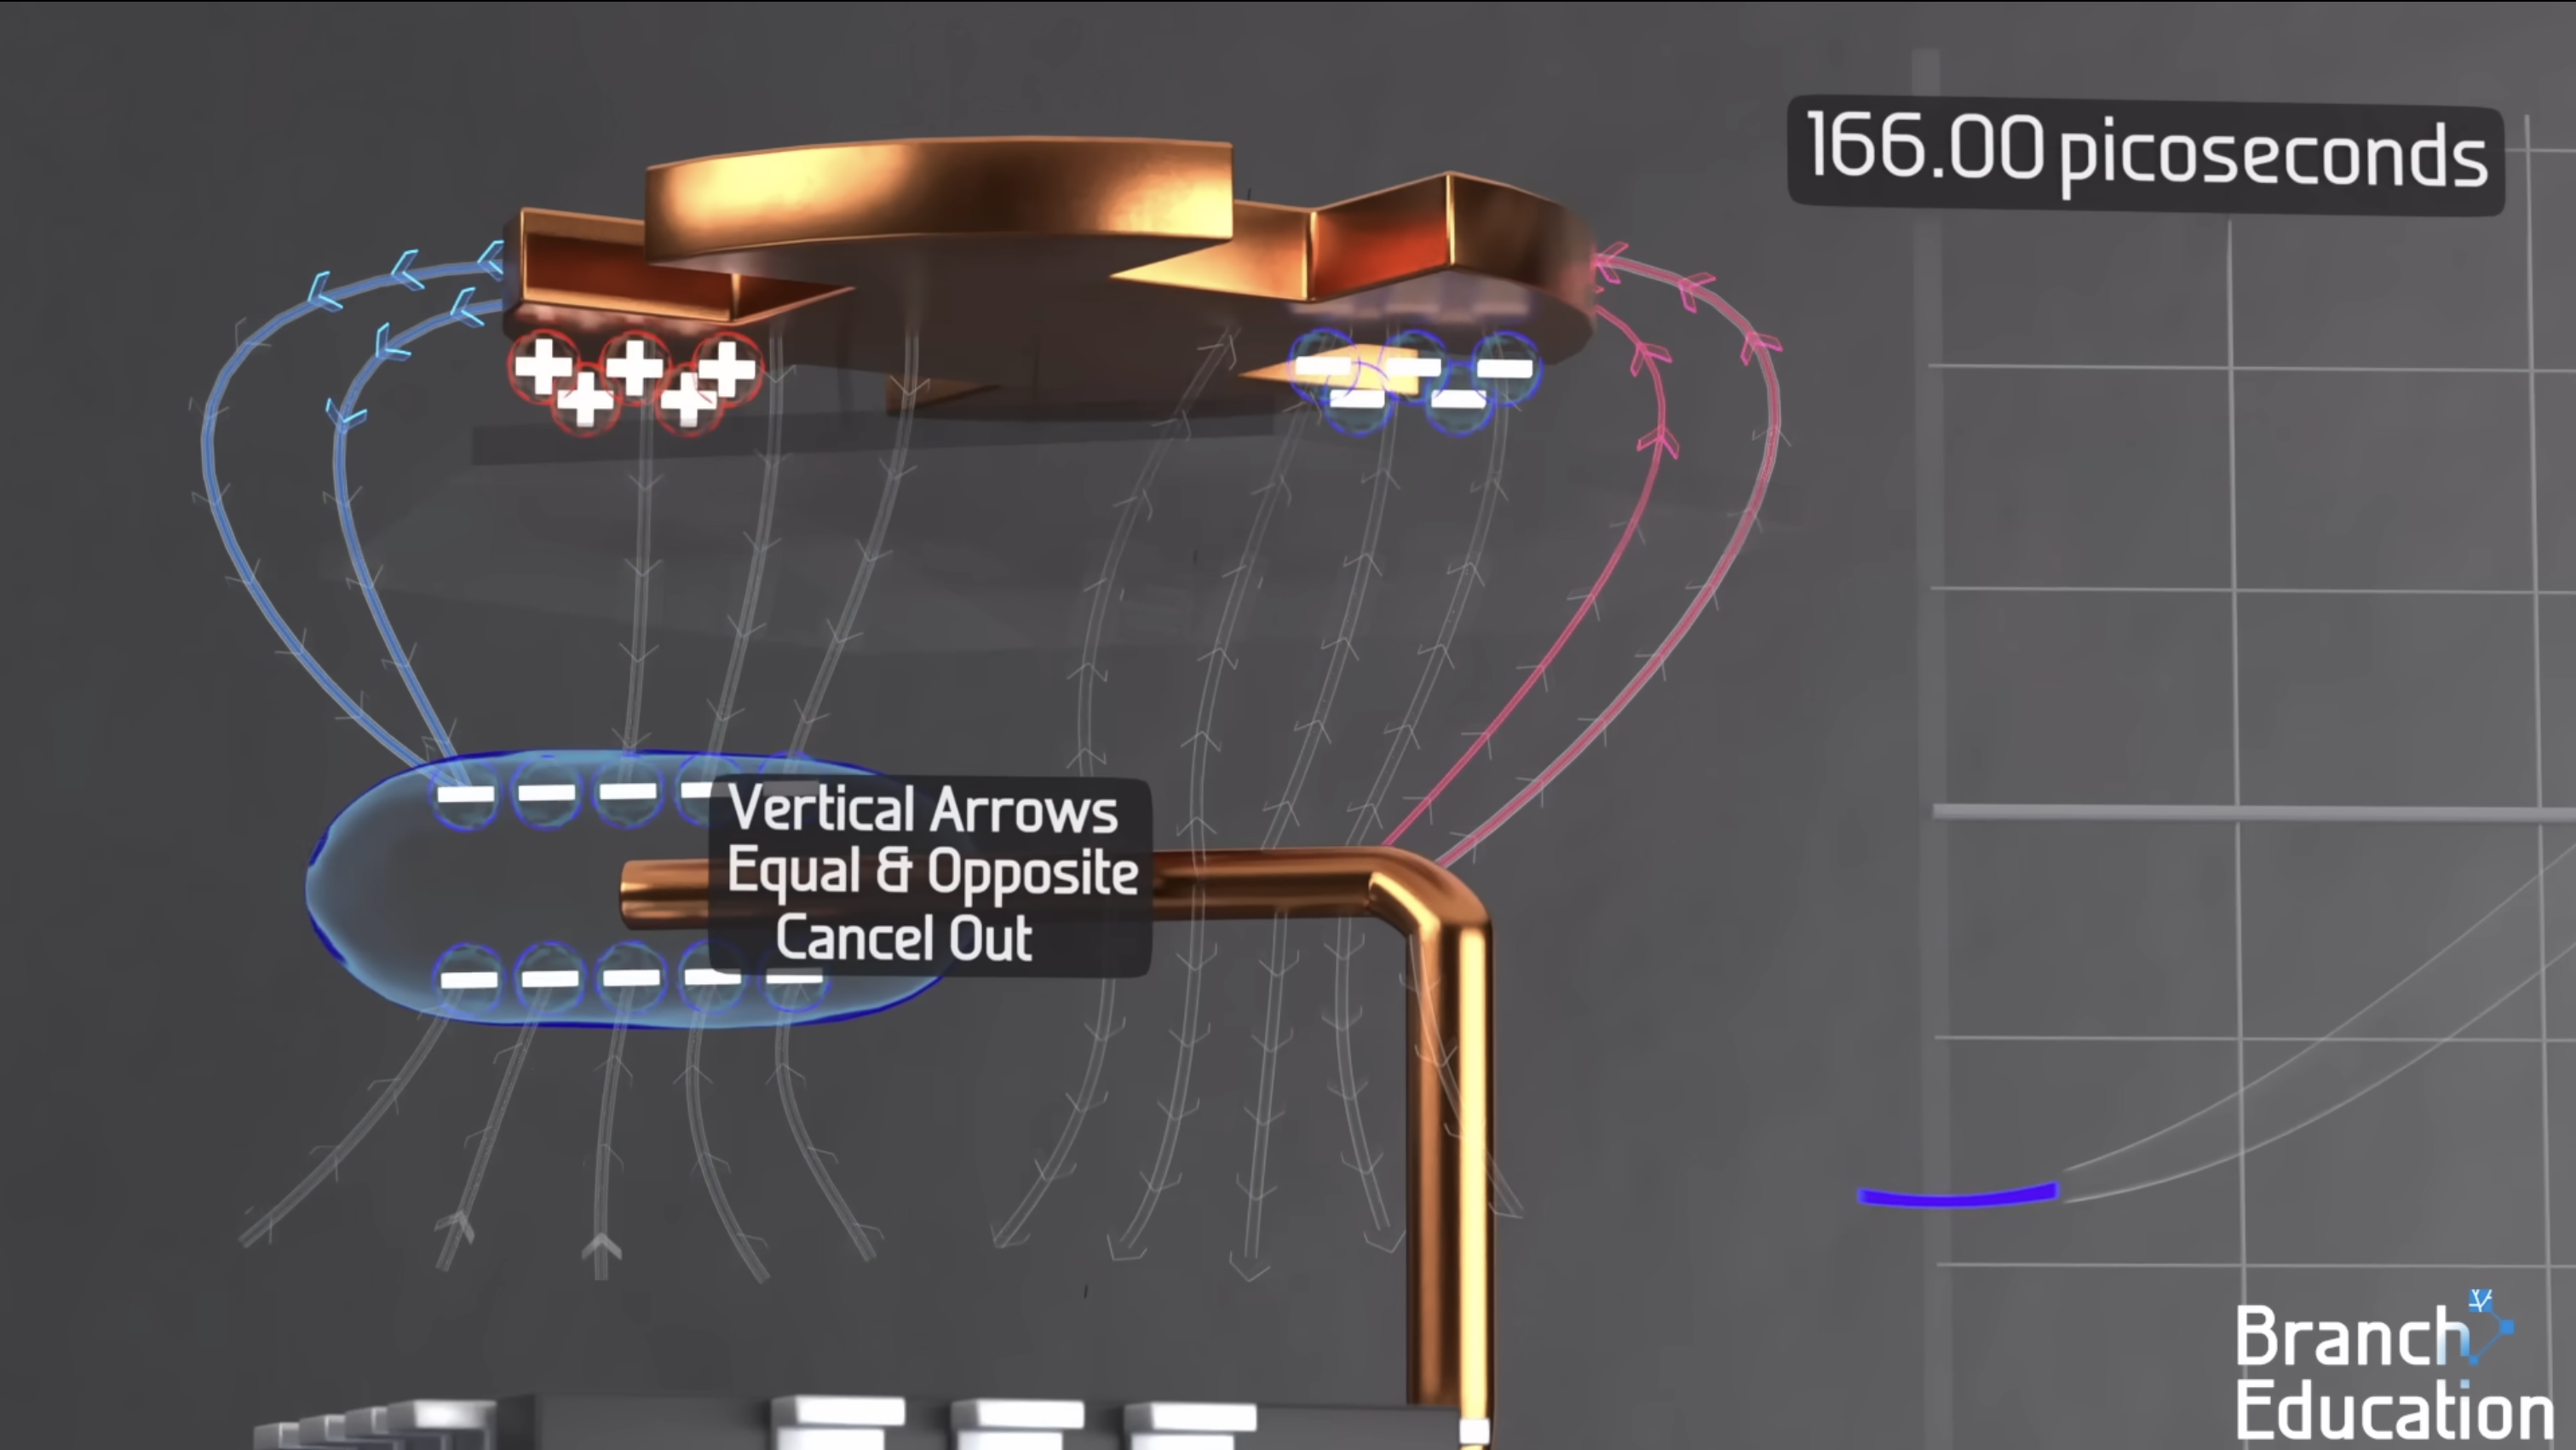
\includegraphics[width=0.8\linewidth]{./res/img/antenna_fringing_fields.png}
  \caption{Creazione dei campi di frangia in un'Aperture Couple Patch antenna \cite{branch_education_how_2022}}
  \label{fig:aperture-couple-patch-antenna-fringing-fields}
\end{figure}

Possiamo vedere in figura \ref{fig:aperture-couple-patch-antenna-fringing-fields} che alcuni di questi vettori di campo elettrico provenienti dal patch sono verticali e, poiché sono uguali e opposti, si annullano.
Tuttavia, altri campi elettrici sono orizzontali nello stesso piano del patch e sono chiamati campi di frangia.
Questi campi di frangia sono nella stessa direzione e quindi si sommano l'uno all'altro, dando luogo a un campo elettrico combinato.

Allo stesso tempo, gli elettroni che scorrono da un lato all'altro del disco, che costituiscono una corrente elettrica, generano un campo magnetico con un'intensità e una direzione, o vettore, perpendicolare al vettore del campo elettrico di frangia.
Di conseguenza, abbiamo un campo elettrico orientato in un senso e un campo magnetico orientato perpendicolarmente, come si può vedere in figura \ref{fig:aperture-couple-patch-antenna-em-field}.

\begin{figure}[htbp]
  \centering
  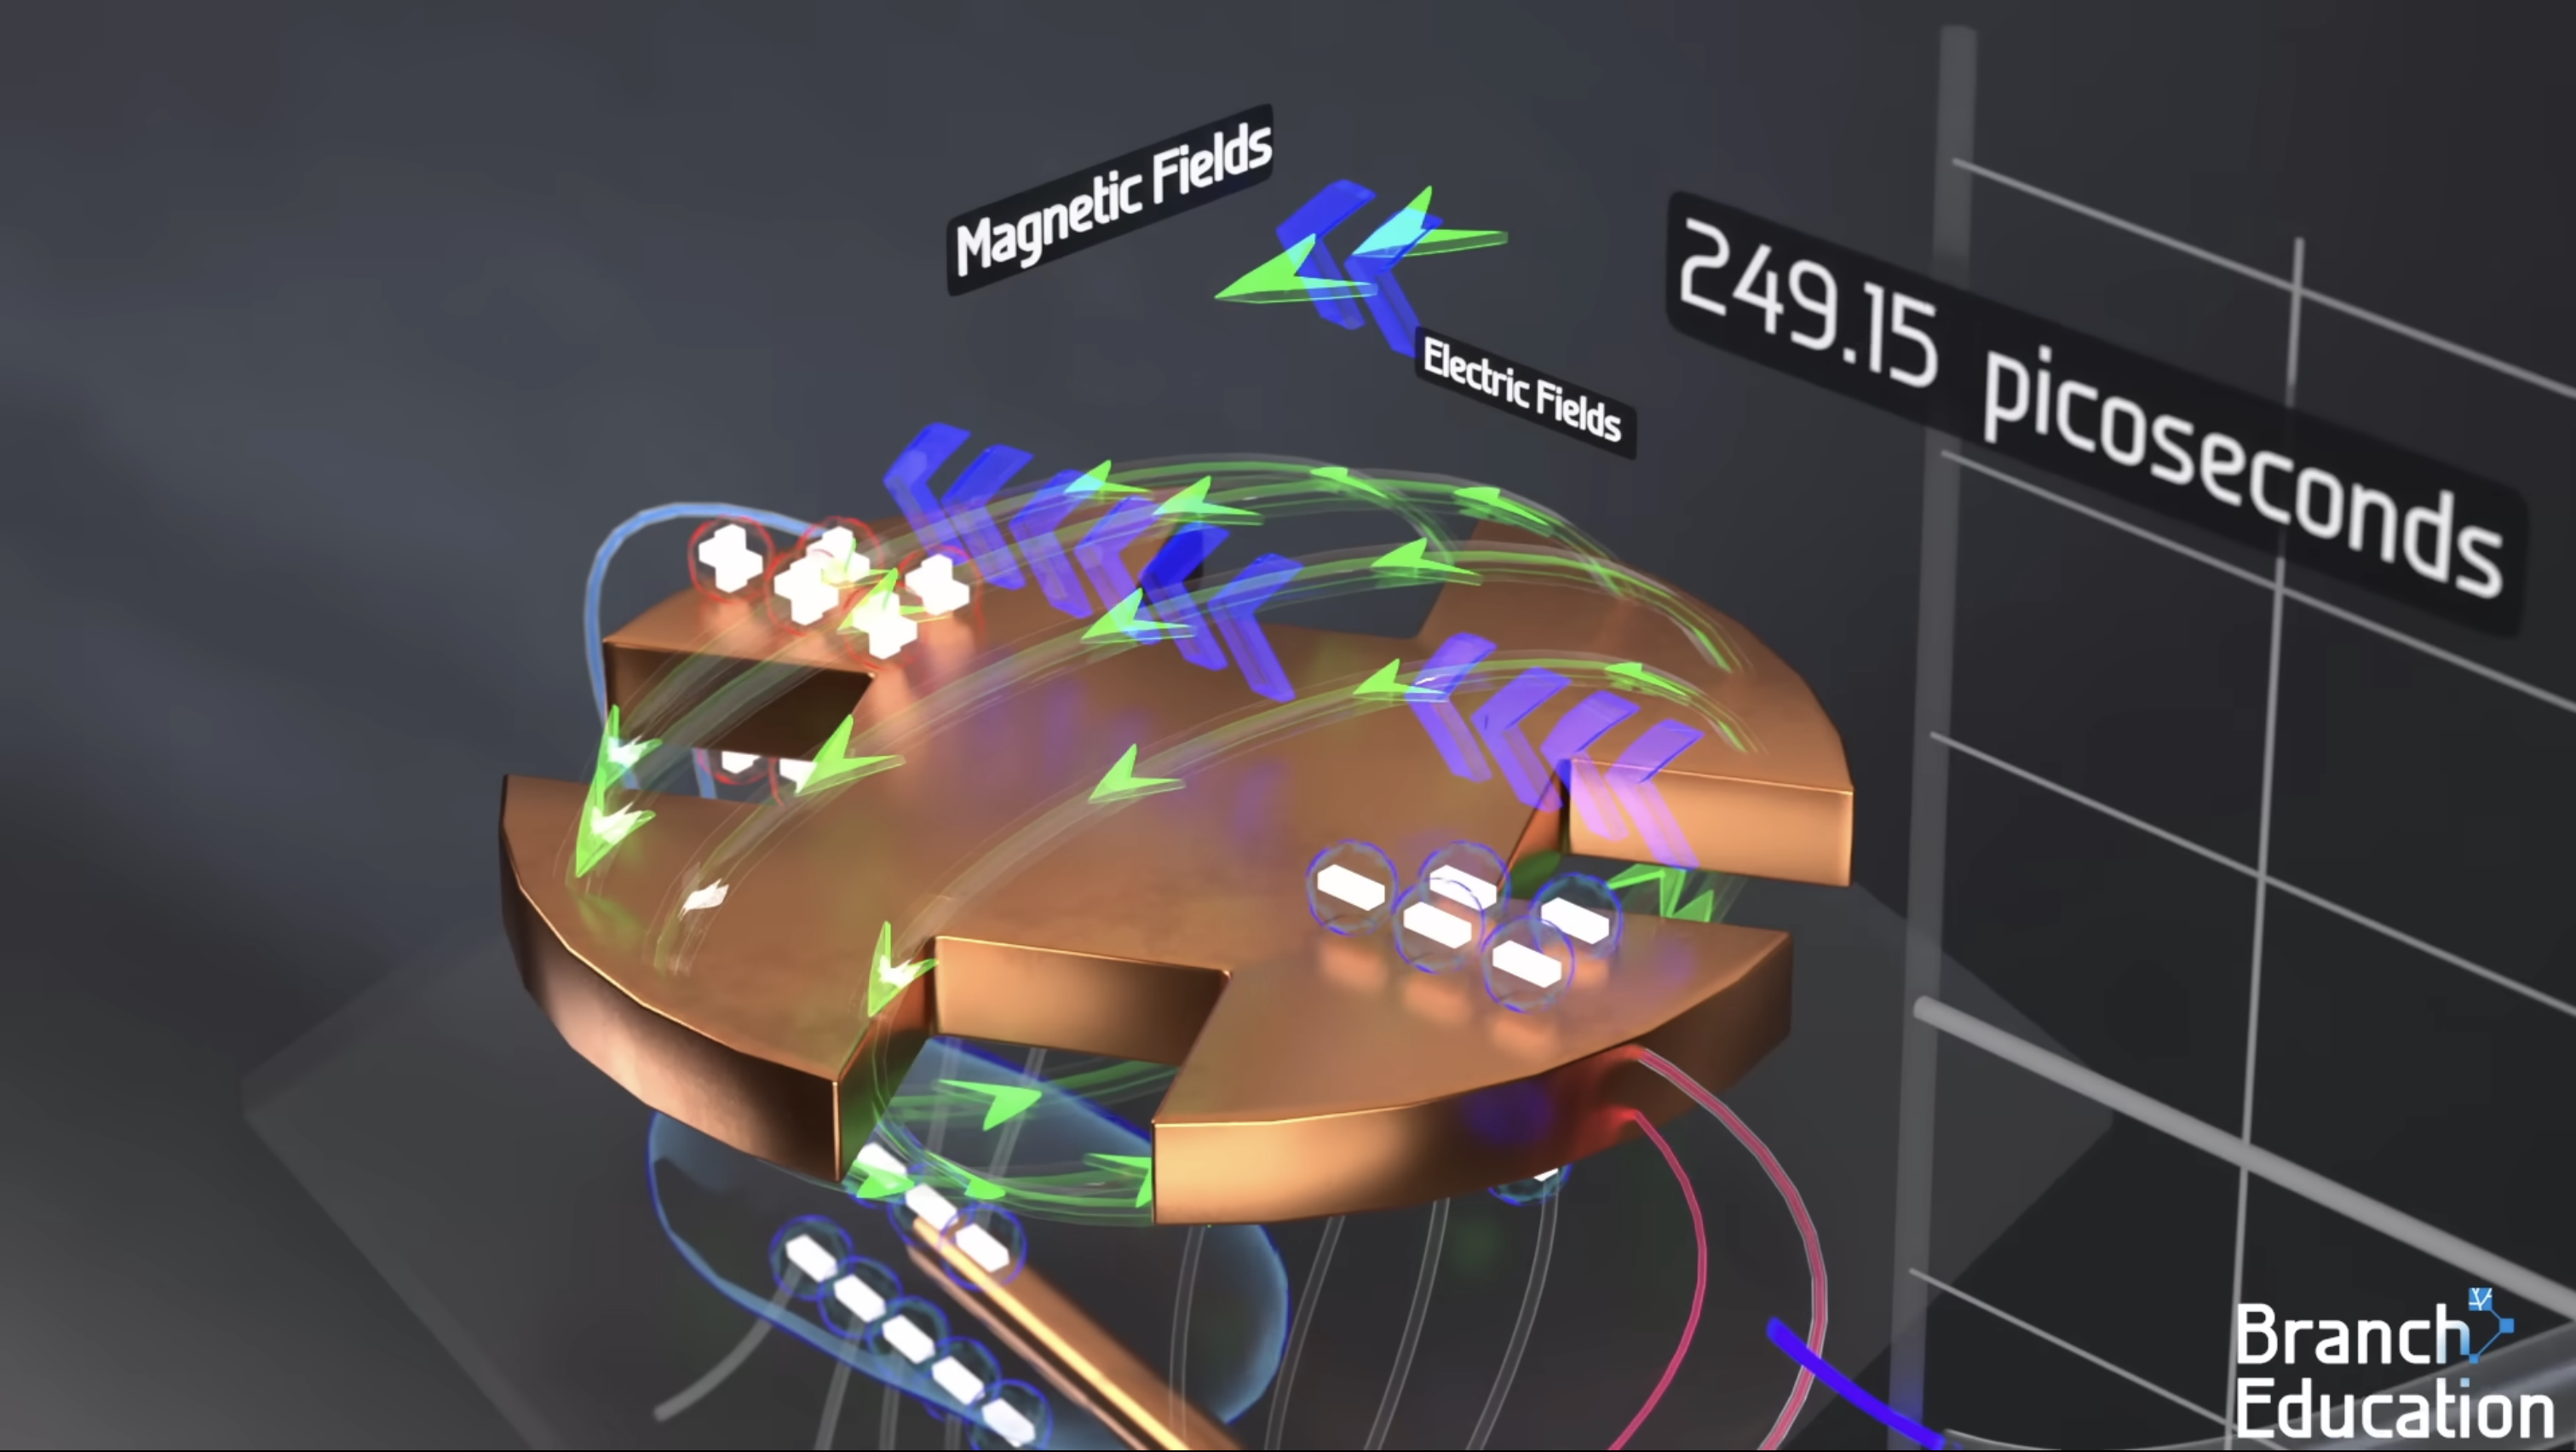
\includegraphics[width=0.8\linewidth]{./res/img/antenna_em_field.png}
  \caption{Campo elettromagnetico in un'Aperture Couple Patch antenna \cite{branch_education_how_2022}}
  \label{fig:aperture-couple-patch-antenna-em-field}
\end{figure}

42 picosecondi dopo, quando la tensione sulla linea di alimentazione diventa positiva, e siamo al picco della sinusoide, la tensione e la corrente sono invertite.
Quindi il campo elettrico e quello magnetico puntano alla direzione opposta.

\subsubsection{Emissione delle onde elettromagnetiche}
Creando i campi elettromagnetici oscillanti vengono generate onde elettromagnetiche che viaggiano in direzione perpendicolare al campo elettrico e al campo magnetico.
Dato che i due insiemi di campi vettoriali non sono tutti sullo stesso piano, ma sono curvati, l'onda elettromagnetica che si propaga viaggia verso l'esterno in una forma di guscio che si espande.

L'intensità di questi campi vettoriali è legata direttamente alla tensione che è stata originariamente mandata alla linea di alimentaizone alla base dell'antenna.

% QUI QUI QUI 10:09 video



% NUMERO DI SATELLITI, COME AVVIENE COMUNICAZIONE UTENTE-UTENTE E UTENTE-SATELLITE
    %!TEX root = ../main.tex

\chapter{Antenna}

\section{Struttura generale}
Aprendo la parabola (versione 1.0 revisione 2) troviamo sul retro una coppia di motori e un cavo ethernet che si collega al router.
Questi motori non muovono continuamente la parabola per puntare direttamente al satellite con cui comunica; vengono utilizzati solo durante la configurazione iniziale per orientare l'antenna nella direzione generale corretta.
Aprendo la parabola troviamo una piastra posteriore strutturale in alluminio e, dall'altro lato, una grande scheda a circuiti stampati (PCB).
Su un lato ci sono 640 microchip piccoli e 20 microchip più grandi, disposti in un pattern con tracce che si diramano dai microchip più grandi a quelli più piccoli, insieme a chp aggiuntivi, inclusa la CPU principale e il modulo GPS sul bordo del PCB. Sull'altro lato cisono circa 1400 cerchi di rame con una griglia di quadrati tra i cerchi.
Nel livello successivo c'è uno schema a nido d'ape in gomma con piccoli cerchi di rame intagliati e dietro troviamo un altro schema a nido d'ape e poi la copertura anteriore della parabola.
Abbiamo quindi 1280 antenne disposte in un pattern esagonale a nido d'ape, con ciascuna pila di cerchi di rame che rappresenta una singola antenna controllata dai microchip sul PCB.
Questo enorme array funziona insieme in quella che è chiamata un'antenna phased array per inviare e ricevere onde elettromagnetiche che vengono direzionate verso e da un satellite Starlink in orbita a 550km di distanza \cite{branch_education_how_2022}.

\subsection{Funzionamento dell'antenna Aperture Couple Patch}

\begin{figure}[htbp]
  \centering
  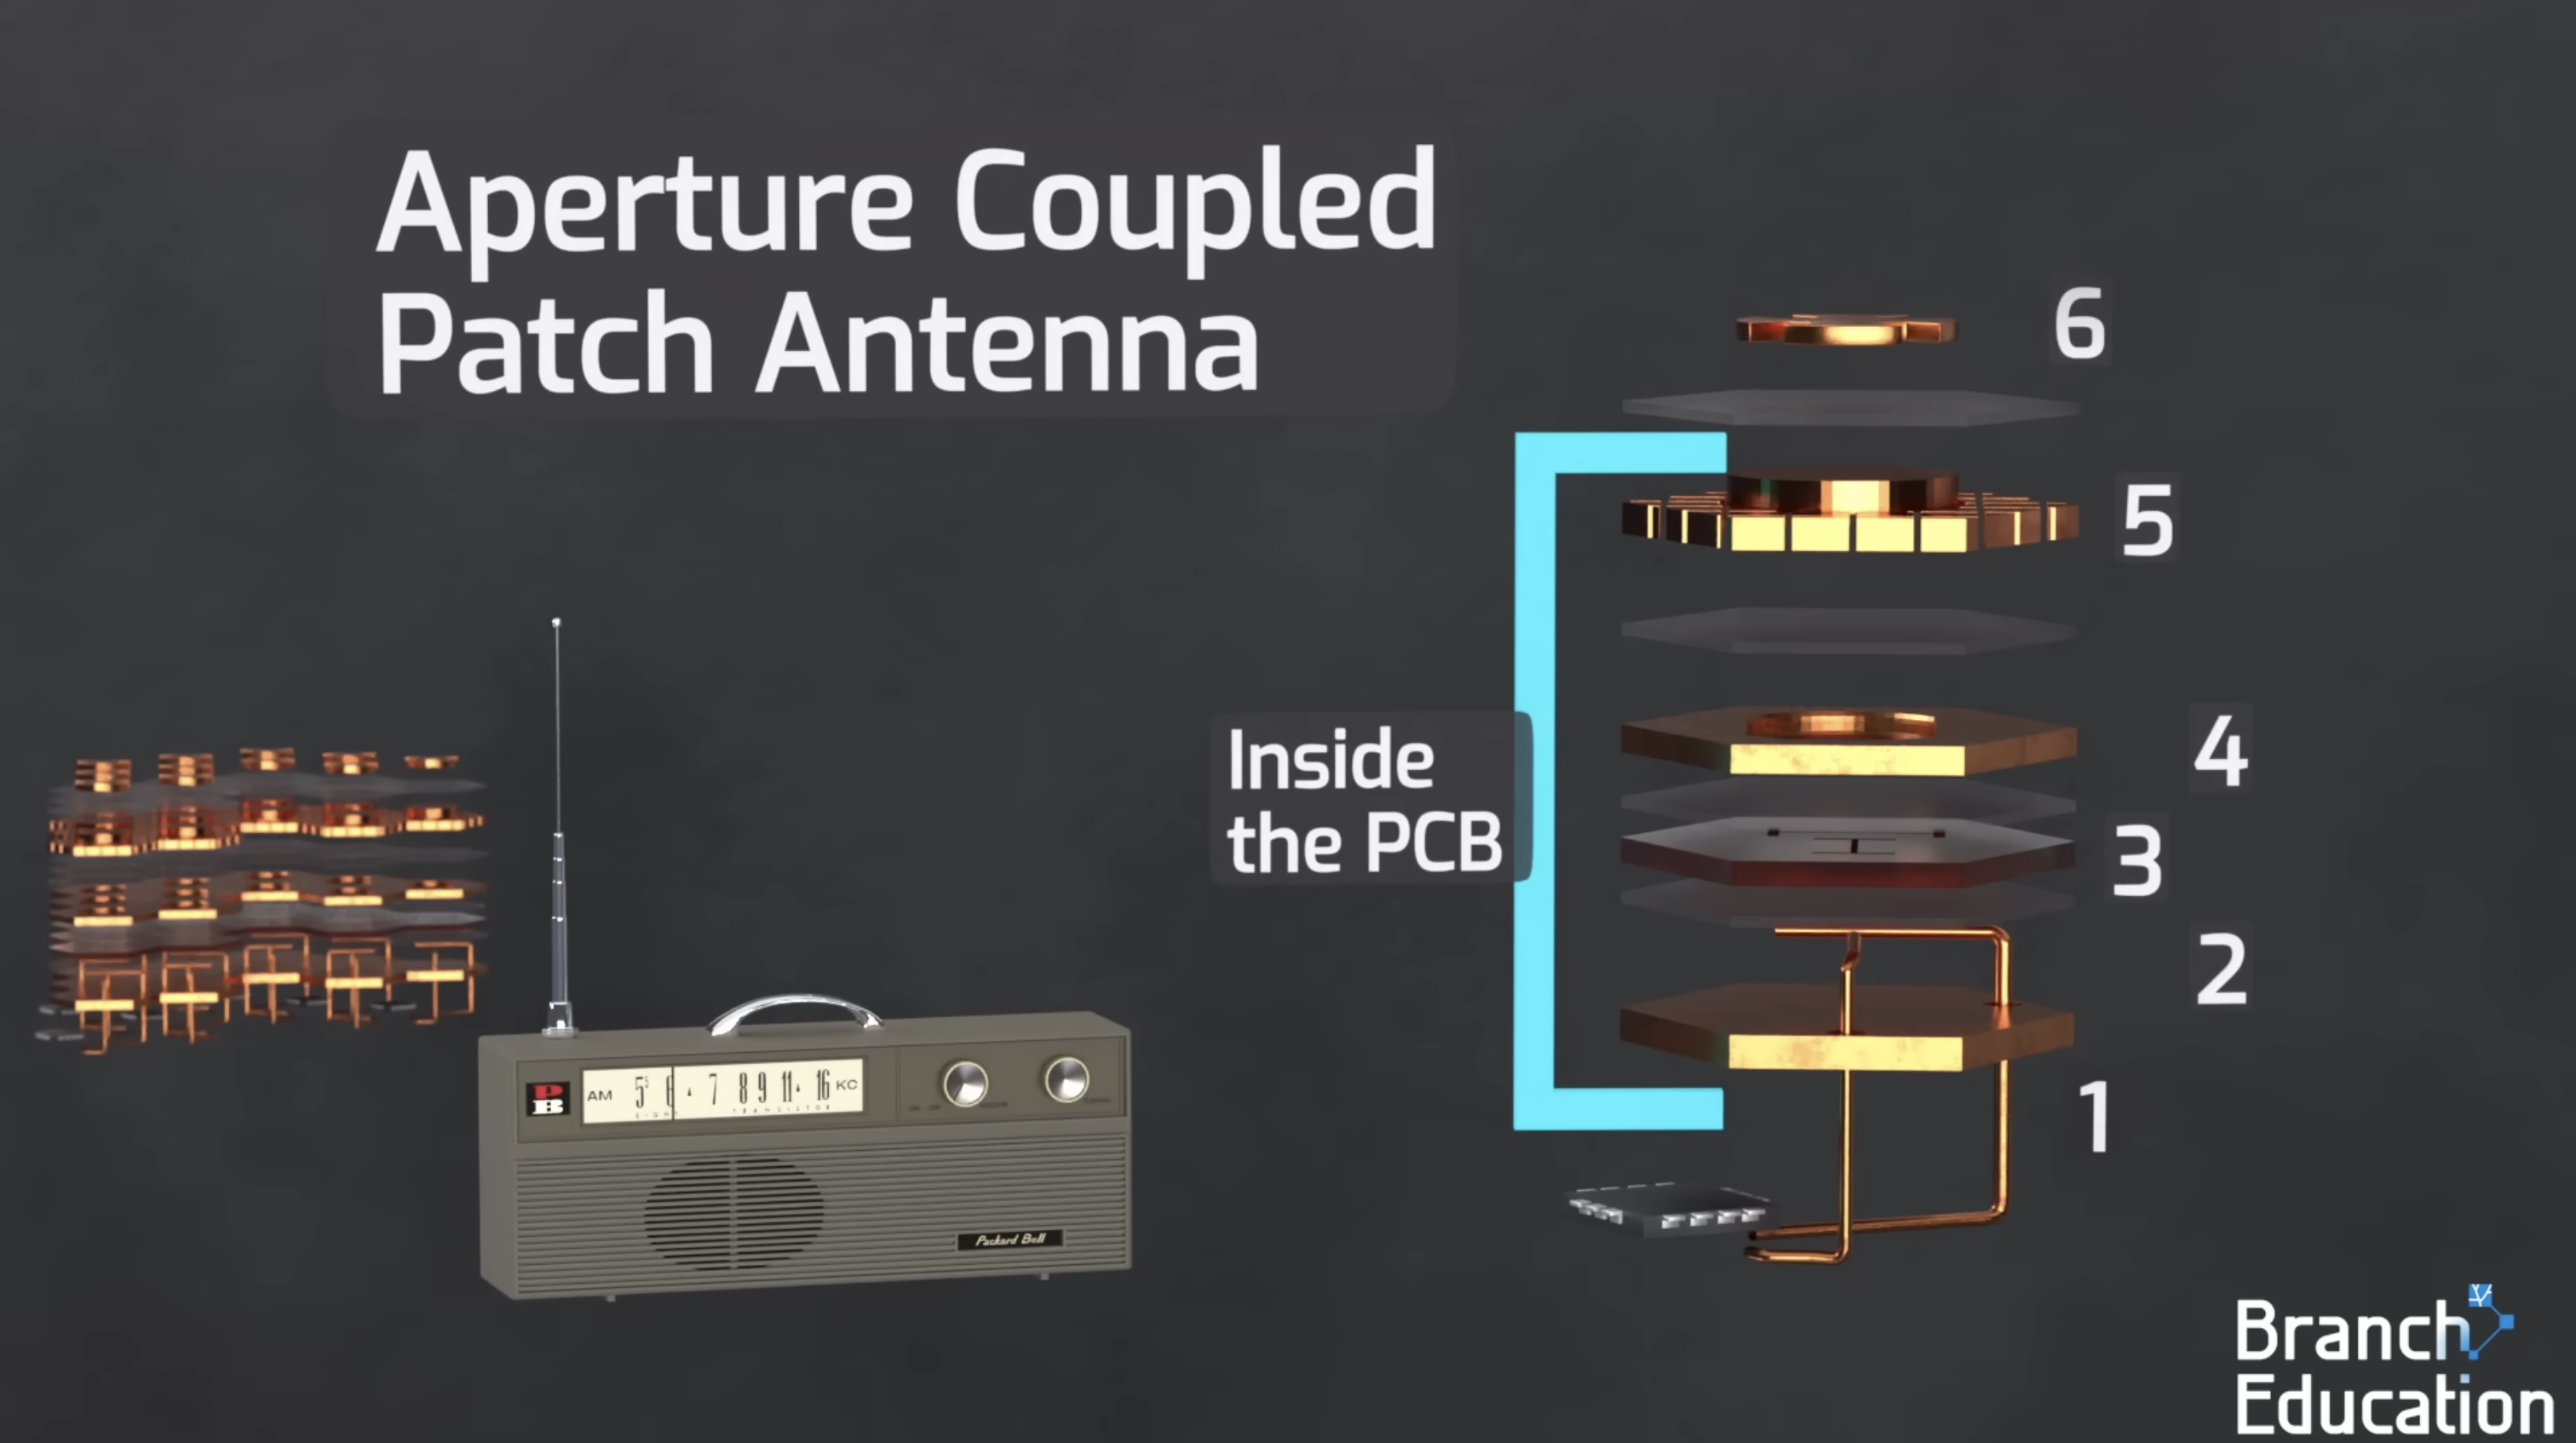
\includegraphics[width=0.8\linewidth]{./res/img/antenna_pcb.png}
  \caption{Aperture Couple Patch antenna \cite{branch_education_how_2022}}
  \label{fig:aperture-couple-patch-antenna}
\end{figure}

Nella figura \ref{fig:aperture-couple-patch-antenna} possiamo vedere un'aperture couple patch antenna, composta di 6 layer, il più dei quali all'interno del PCB.
I layer più importanti sono:
\begin{itemize}
  \item[1.] linea di alimentazione.
  \item[2.] piano RF reflective.
  \item[3.] H slot per la polarizzazione.
  \item[4.] isolamento dell'antenna.
  \item[5.] Bottom antenna patch: trasmettitore a 13 GHz.
  \item[6.] Top antenna patch: ricevitore a 11.7 GHz.
\end{itemize}
I pezzi esagonali grigio scuro invece sono isolamento elettrico tra i vari layer \cite{branch_education_how_2022}.

Per facilitare la comprensione del suo funzionamento semplifichiamola rimuovendo per il momento alcuni layer, e vediamo i principi base di come si genera un'onda elettromagnetica che si propaga da quest'antenna.

Per iniziare, sul fondo abbiamo una micro linea di trasmissione elettrica che arriva da uno dei piccoli microchip.
Questa linea di trasmissione è solo un filo di rame che termina sotto la pila dell'antenna.
Mandiamo una tensione sinusodiale alla frequenza di 12 GHz al filo di alimentazione, quindi con un periodo di 83 pico secondi.
Al di sopra del filo di rame di alimentazione abbiamo un cerchio di rame con intagli chiamato patch d'antenna.

Con la corrente continua o alternata a bassa frequenza, non succederebbe molto perchè il patch è isolato, ma con un segnale ad alta frequenza la potenza inviata al filo di alimentazione viene accoppiata o inviata al patch.
Questo fenomeno avviene perchè quando la tensione è al fondo della sua sinusoide, o al minimo, c'è una concentrazione di elettroni spinti verso l'estremità del filo di alimentazione, creando così una zona di carica negativa che corrisponde alla massima tensione negativa.
Questa concentrazione di elettroni sulla punta del filo respinge tutti gli elettroni, compresi quelli sulla parte superiore del patch, e di conseguenza questi elettroni vengono spinti verso l'altro lato del patch circolare.
In questo modo, un lato del patch diventa carico positivamente, mentre l'altro diventa carico negativamente, creando così campi elettrici tra il patch e il filo di alimentazione.

Tuttavia, quando invertiamo la tensione al filo di rame 41.5 picosecondi dopo, abbiamo una concentrazione di cariche positive, o una mancanza di elettroni all'estremità del filo, e quindi gli elettroni nel patch fluiscono verso l'altro lato. La tensione nel patch è invertita e quindi anche la direzione dei campi elettrici è invertita \cite{branch_education_how_2022}.

\begin{figure}[htbp]
  \centering
  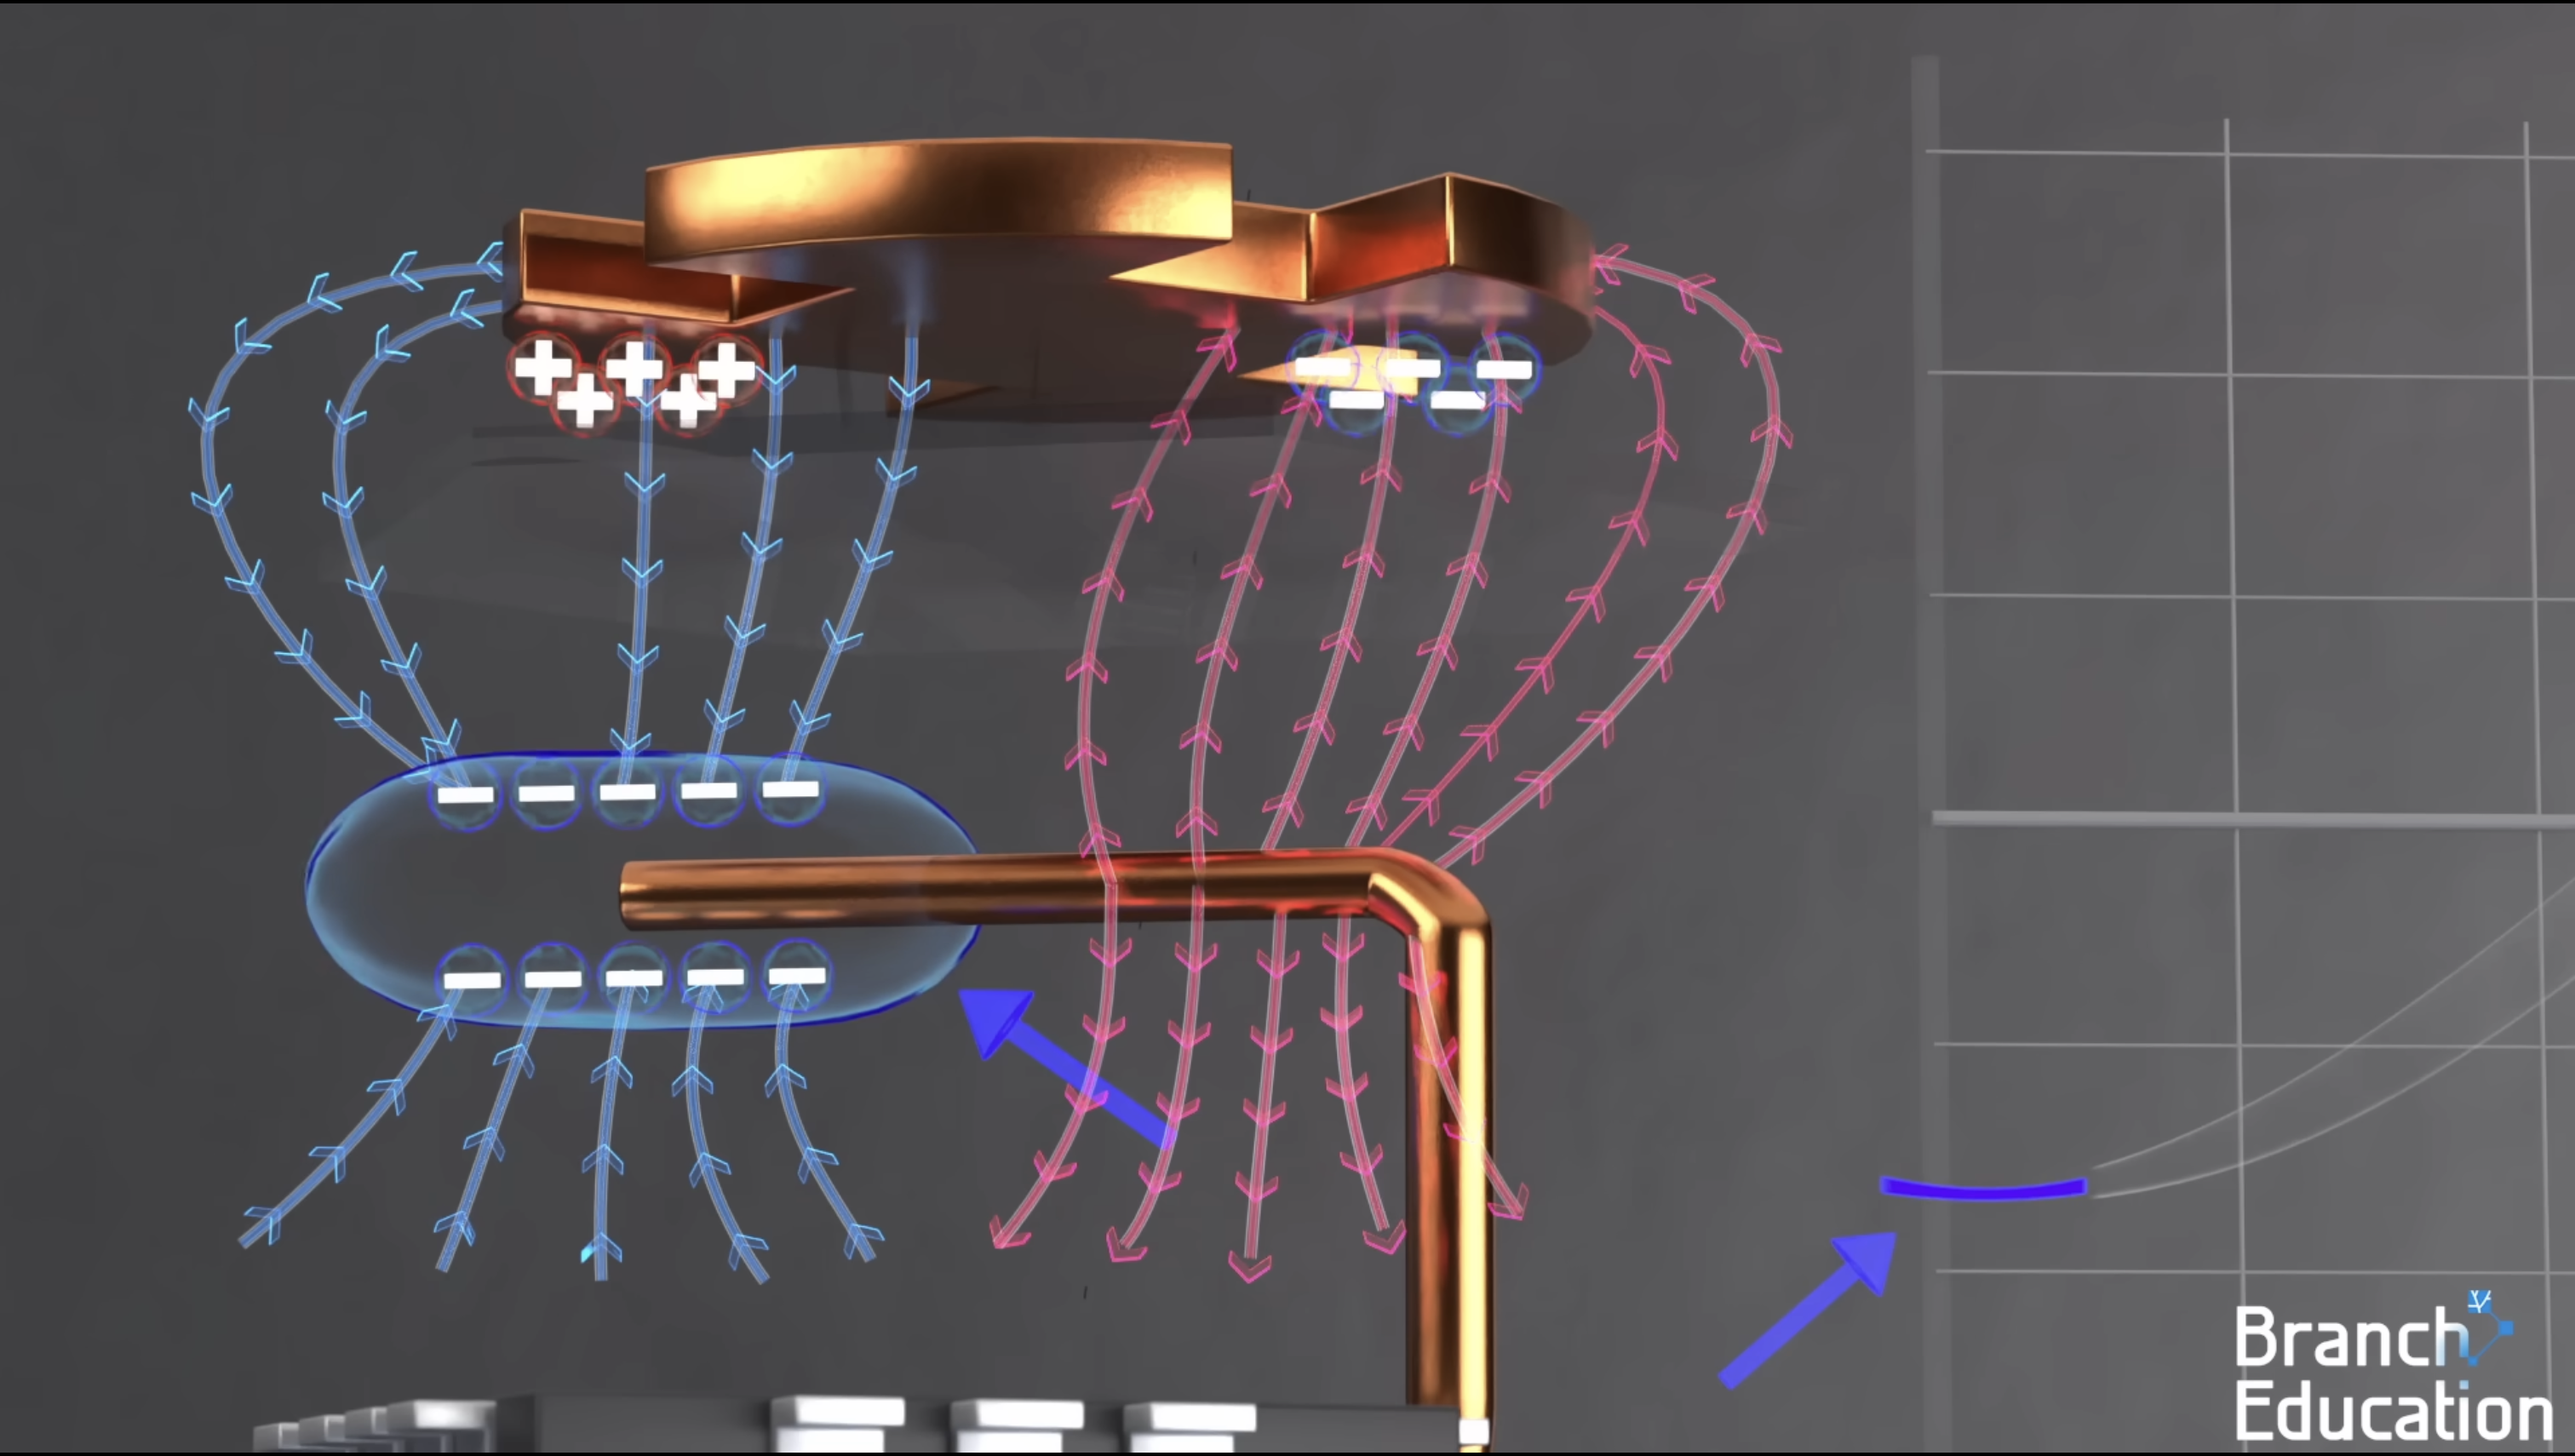
\includegraphics[width=0.8\linewidth]{./res/img/antenna_voltage_applied.png}
  \caption{Aperture Couple Patch antenna con un segnale applicato \cite{branch_education_how_2022}}
  \label{fig:aperture-couple-patch-antenna-voltage-applied}
\end{figure}

Poiché la tensione del filo di alimentazione oscilla con un intervallo di 41.5 picosecondi tra un picco e un avvallamento, anche i campi elettrici nel patch oscilleranno mentre gli elettroni vanno avanti e indietro.

\begin{figure}[htbp]
  \centering
  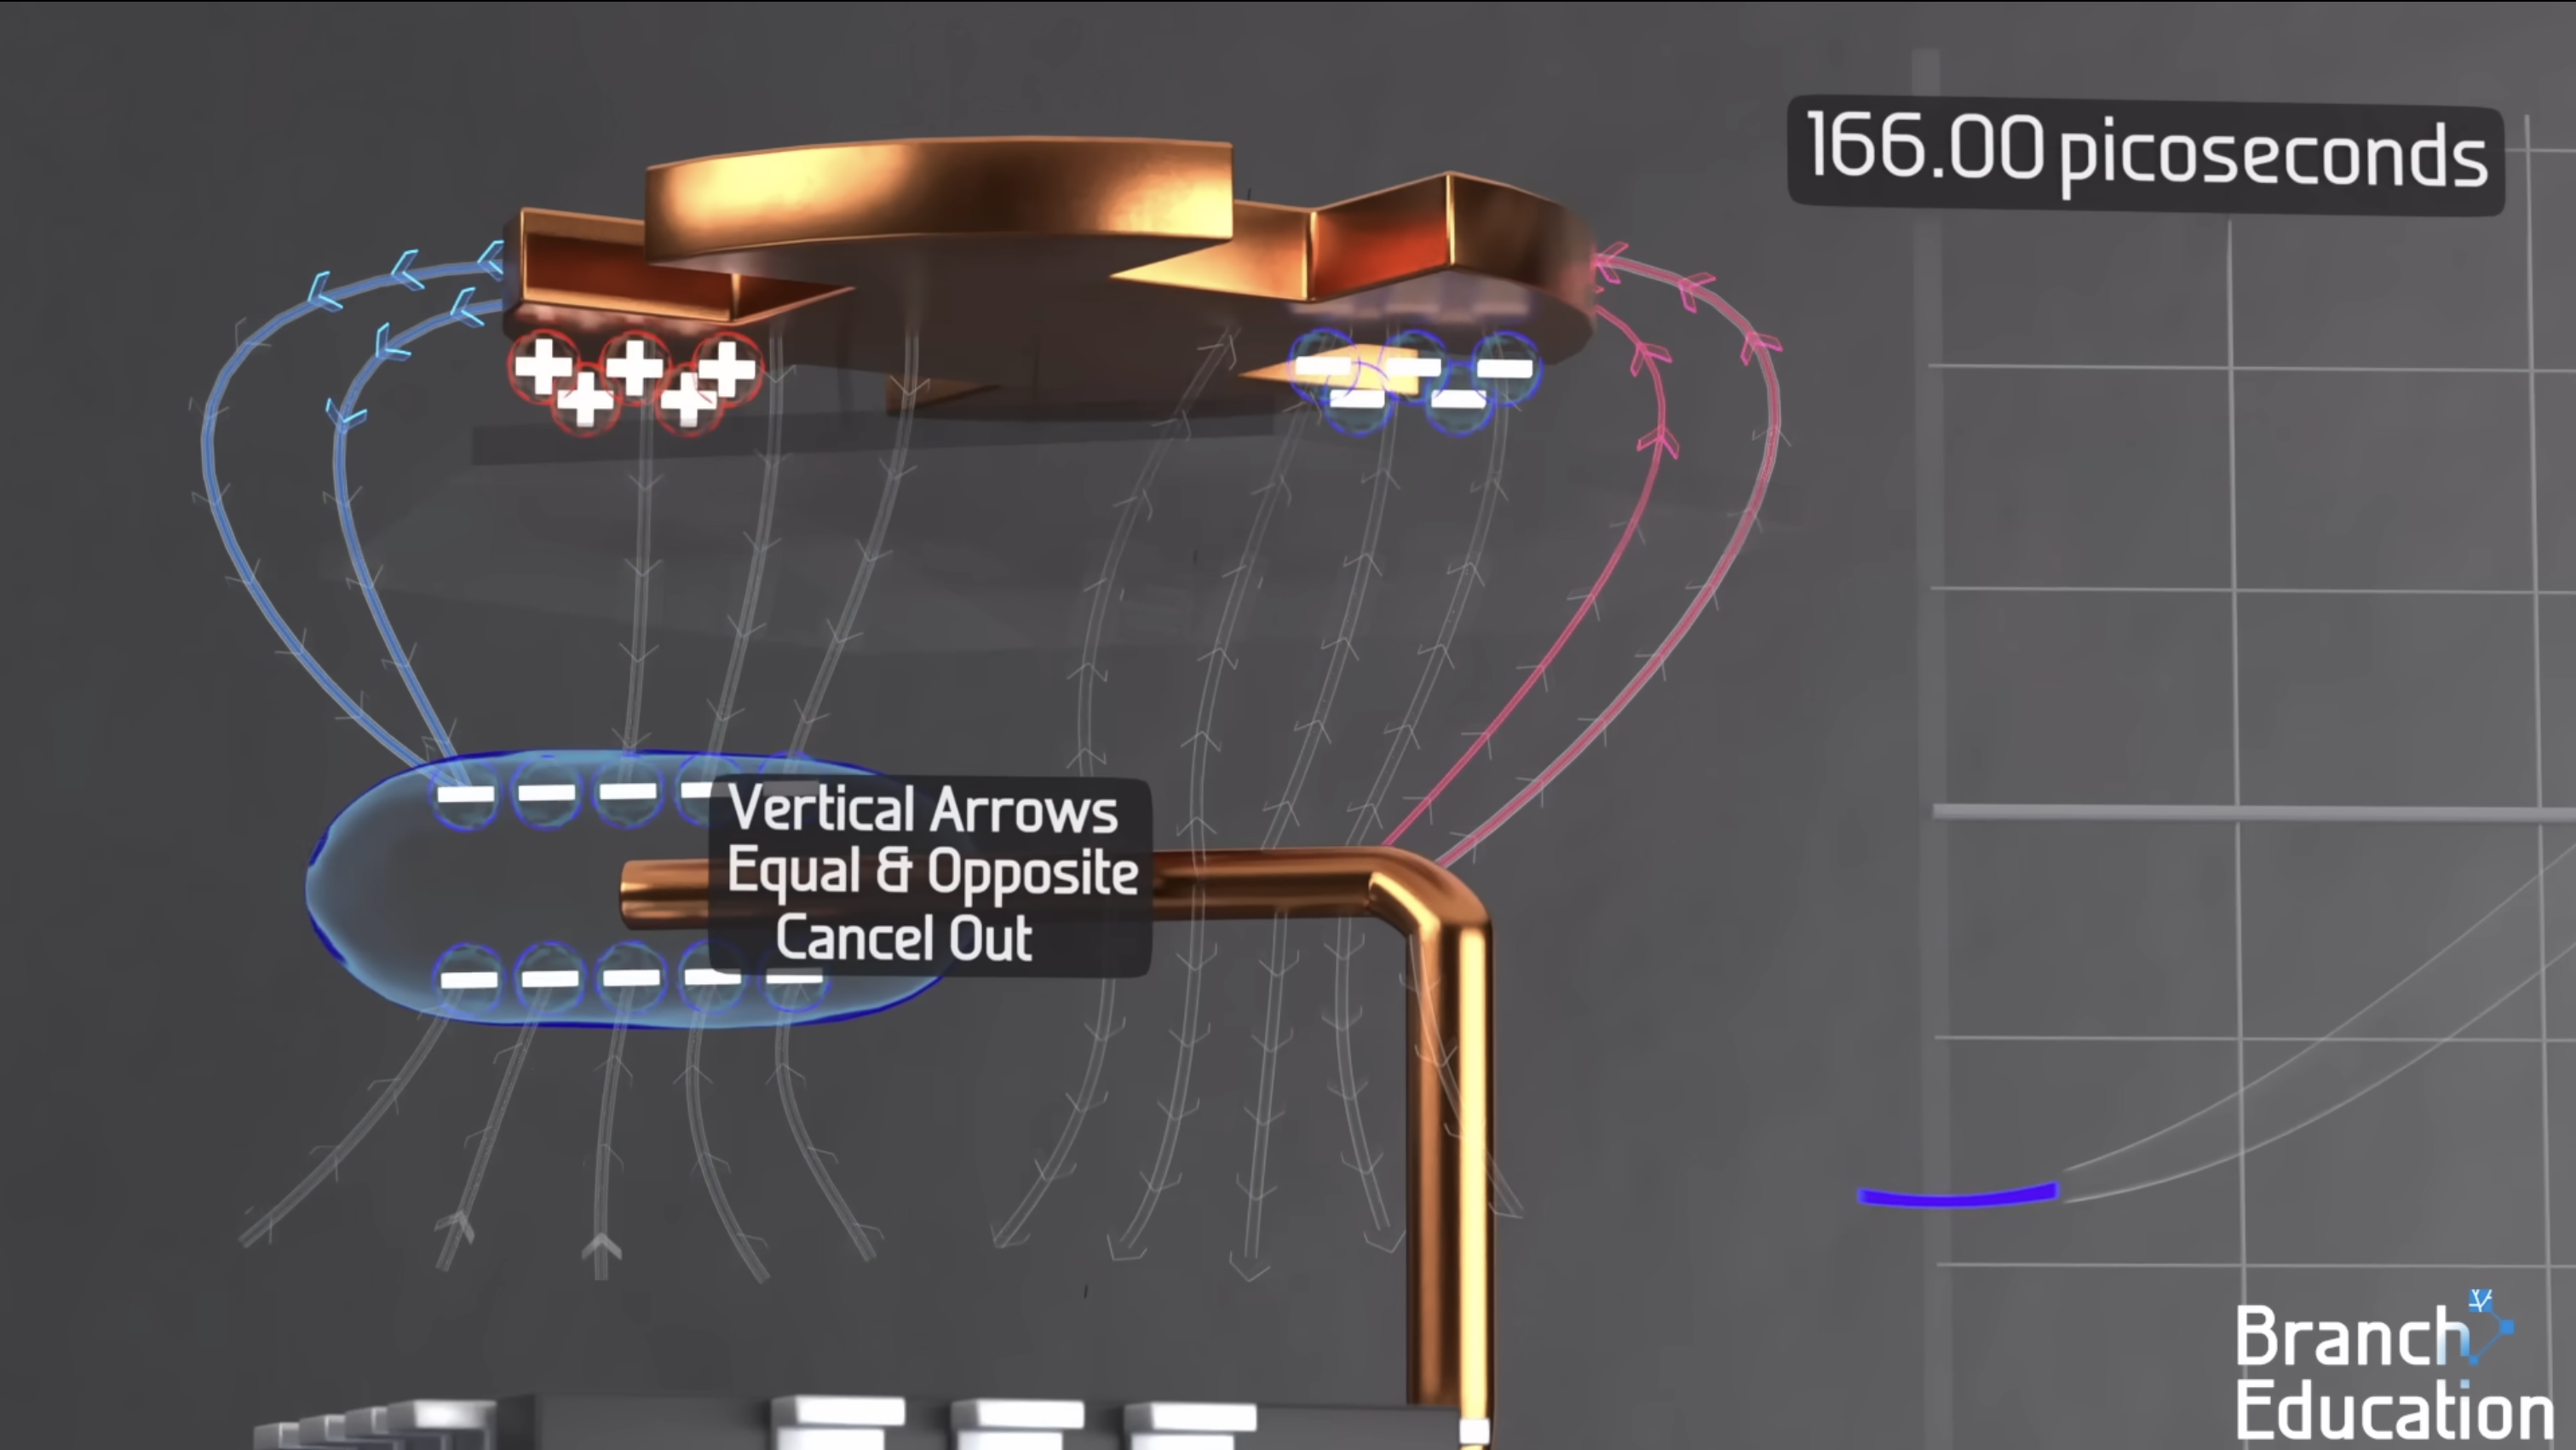
\includegraphics[width=0.8\linewidth]{./res/img/antenna_fringing_fields.png}
  \caption{Creazione dei campi di frangia in un'Aperture Couple Patch antenna \cite{branch_education_how_2022}}
  \label{fig:aperture-couple-patch-antenna-fringing-fields}
\end{figure}

Possiamo vedere in figura \ref{fig:aperture-couple-patch-antenna-fringing-fields} che alcuni di questi vettori di campo elettrico provenienti dal patch sono verticali e, poiché sono uguali e opposti, si annullano.
Tuttavia, altri campi elettrici sono orizzontali nello stesso piano del patch e sono chiamati campi di frangia.
Questi campi di frangia sono nella stessa direzione e quindi si sommano l'uno all'altro, dando luogo a un campo elettrico combinato \cite{branch_education_how_2022}.

Allo stesso tempo, gli elettroni che scorrono da un lato all'altro del disco, che costituiscono una corrente elettrica, generano un campo magnetico con un'intensità e una direzione, o vettore, perpendicolare al vettore del campo elettrico di frangia.
Di conseguenza, abbiamo un campo elettrico orientato in un senso e un campo magnetico orientato perpendicolarmente, come si può vedere in figura \ref{fig:aperture-couple-patch-antenna-em-field} \cite{branch_education_how_2022}.

\begin{figure}[htbp]
  \centering
  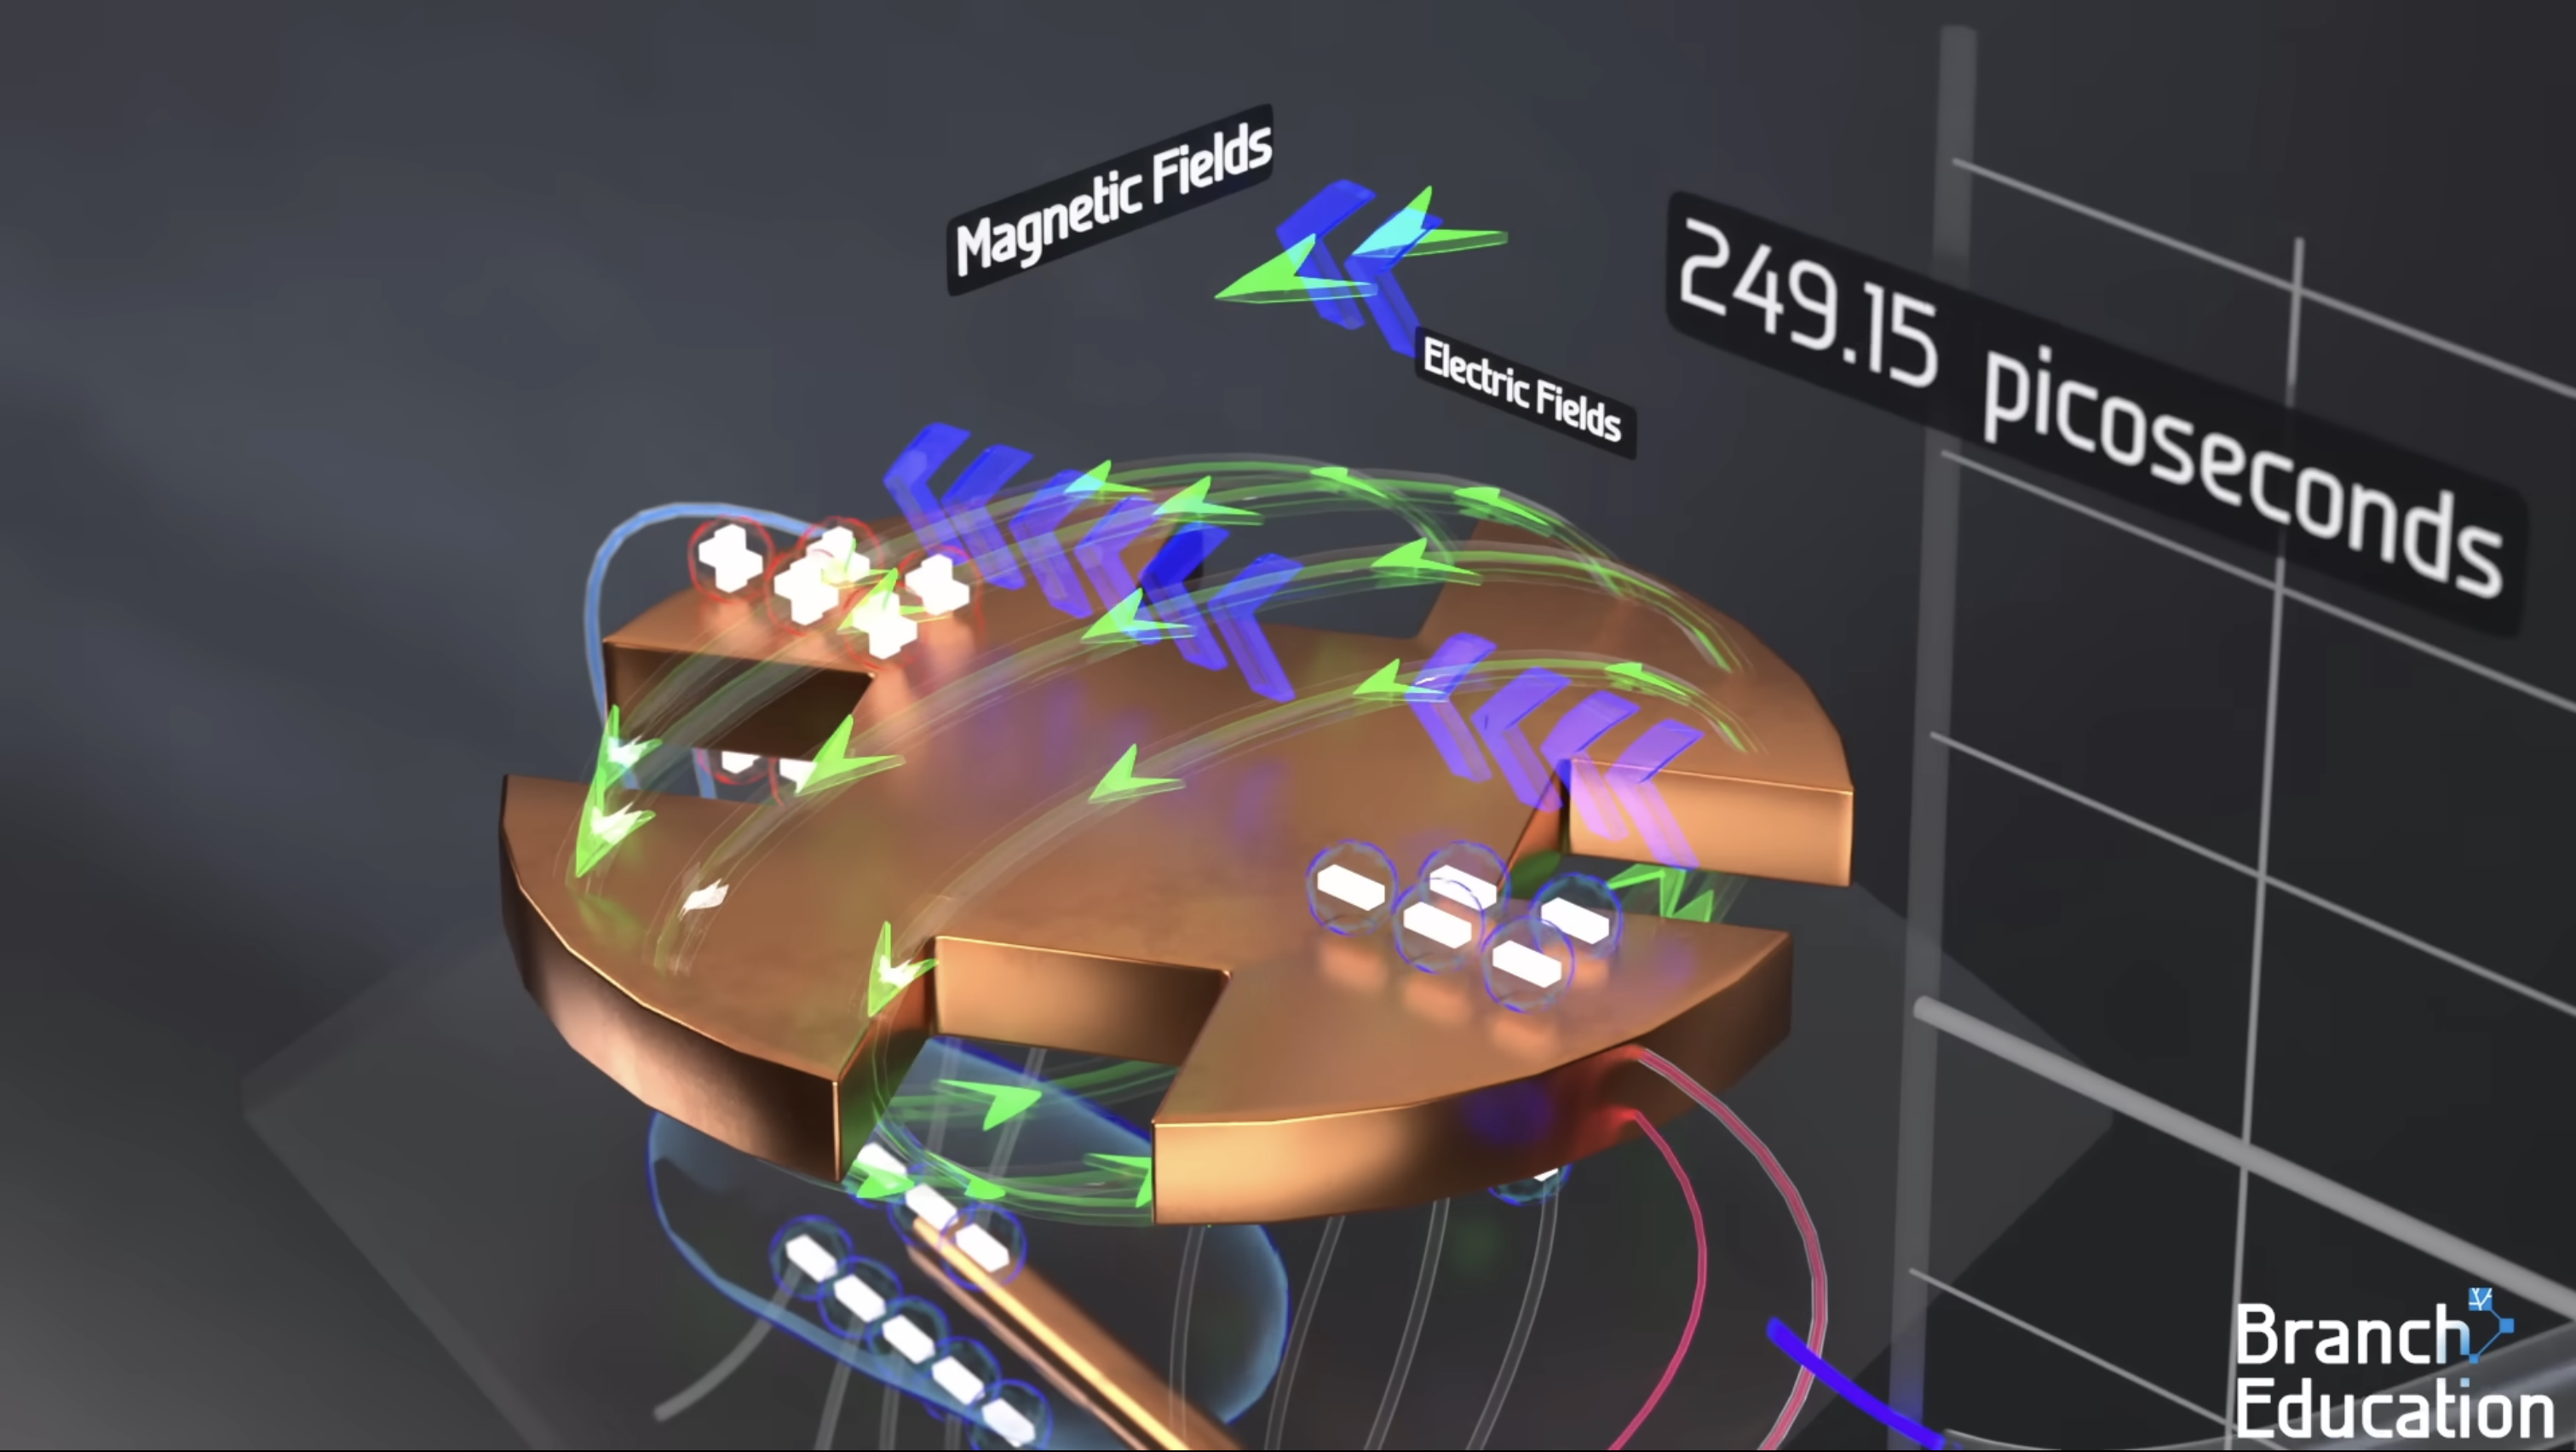
\includegraphics[width=0.8\linewidth]{./res/img/antenna_em_field.png}
  \caption{Campo elettromagnetico in un'Aperture Couple Patch antenna \cite{branch_education_how_2022}}
  \label{fig:aperture-couple-patch-antenna-em-field}
\end{figure}

41.5 picosecondi dopo, quando la tensione sulla linea di alimentazione diventa positiva, e siamo al picco della sinusoide, la tensione e la corrente sono invertite.
Quindi il campo elettrico e quello magnetico puntano alla direzione opposta.

\subsection{Emissione delle onde elettromagnetiche}
Creando i campi elettromagnetici oscillanti vengono generate onde elettromagnetiche che viaggiano in direzione perpendicolare al campo elettrico e al campo magnetico.
Dato che i due insiemi di campi non sono tutti sullo stesso piano, ma sono curvati, l'onda elettromagnetica che si propaga viaggia verso l'esterno in una forma di guscio che si espande.

L'intensità di questi campi è legata direttamente alla tensione che è stata originariamente mandata alla linea di alimentaizone alla base dell'antenna.
Questo significa che se vogliamo rendere questi campi elettromagnetici più intensi basta aumentare la tensione inviata alla linea di alimentazione.

Per ricevere il segnale basta switchare il microchip dell'antenna, chiamato modulo front-end, che si vede in figura \ref{fig:aperture-couple-patch-antenna} da modalità trasmettitore a modalità ricevitore.

Quando un'onda elettromagnetica dal satellite è diretta verso l'antenna, i campi elettromagnetici del segnale in arrivo influenzano gli elettroni nel patch di rame, generando un flusso di elettroni.

Questo segnale ad alta frequenza ricevuto è inviato alla feedline, dove c'è il modulo di front-end che amplifica il segnale.
Quindi, queste antenne possono essere usate sia per trasmettere che per ricevere onde elettromagnetiche, ma non allo stesso tempo \cite{branch_education_how_2022}.

\subsection{Beamforming: come formare un fascio di onde elettromagnetiche che raggiunge lo spazio}
Le tecnica di combinare la potenza delle 1280 antenne in un array esagonale è chiamato beamforming.

Come prima cerchiamo di semplificare il concetto vedendo cosa succede per due antenne affiancate.
Come menzionato prima, un'antenna genera un'onda elettromagnetica che si propaga all'esterno a forma di guscio che si espande.
In ogni singolo punto dello spazio c'è solo un vettore di campo elettrico con un'intensità e una direzione, quindi i vettori di campo elettrico delle due antenne si combinano assieme in tutti i punti nello spazio.
In alcune aree, i campi elettrici delle antenne puntano nella stessa direzione con picchi sovrapposti, e quindi per interferenza costruttiva si sommano.
In altri punti invece sono opposti, con un picco e un'avvallamento, e quindi si cancellano per interferenza distruttiva.

\begin{figure}[htbp]
  \centering
  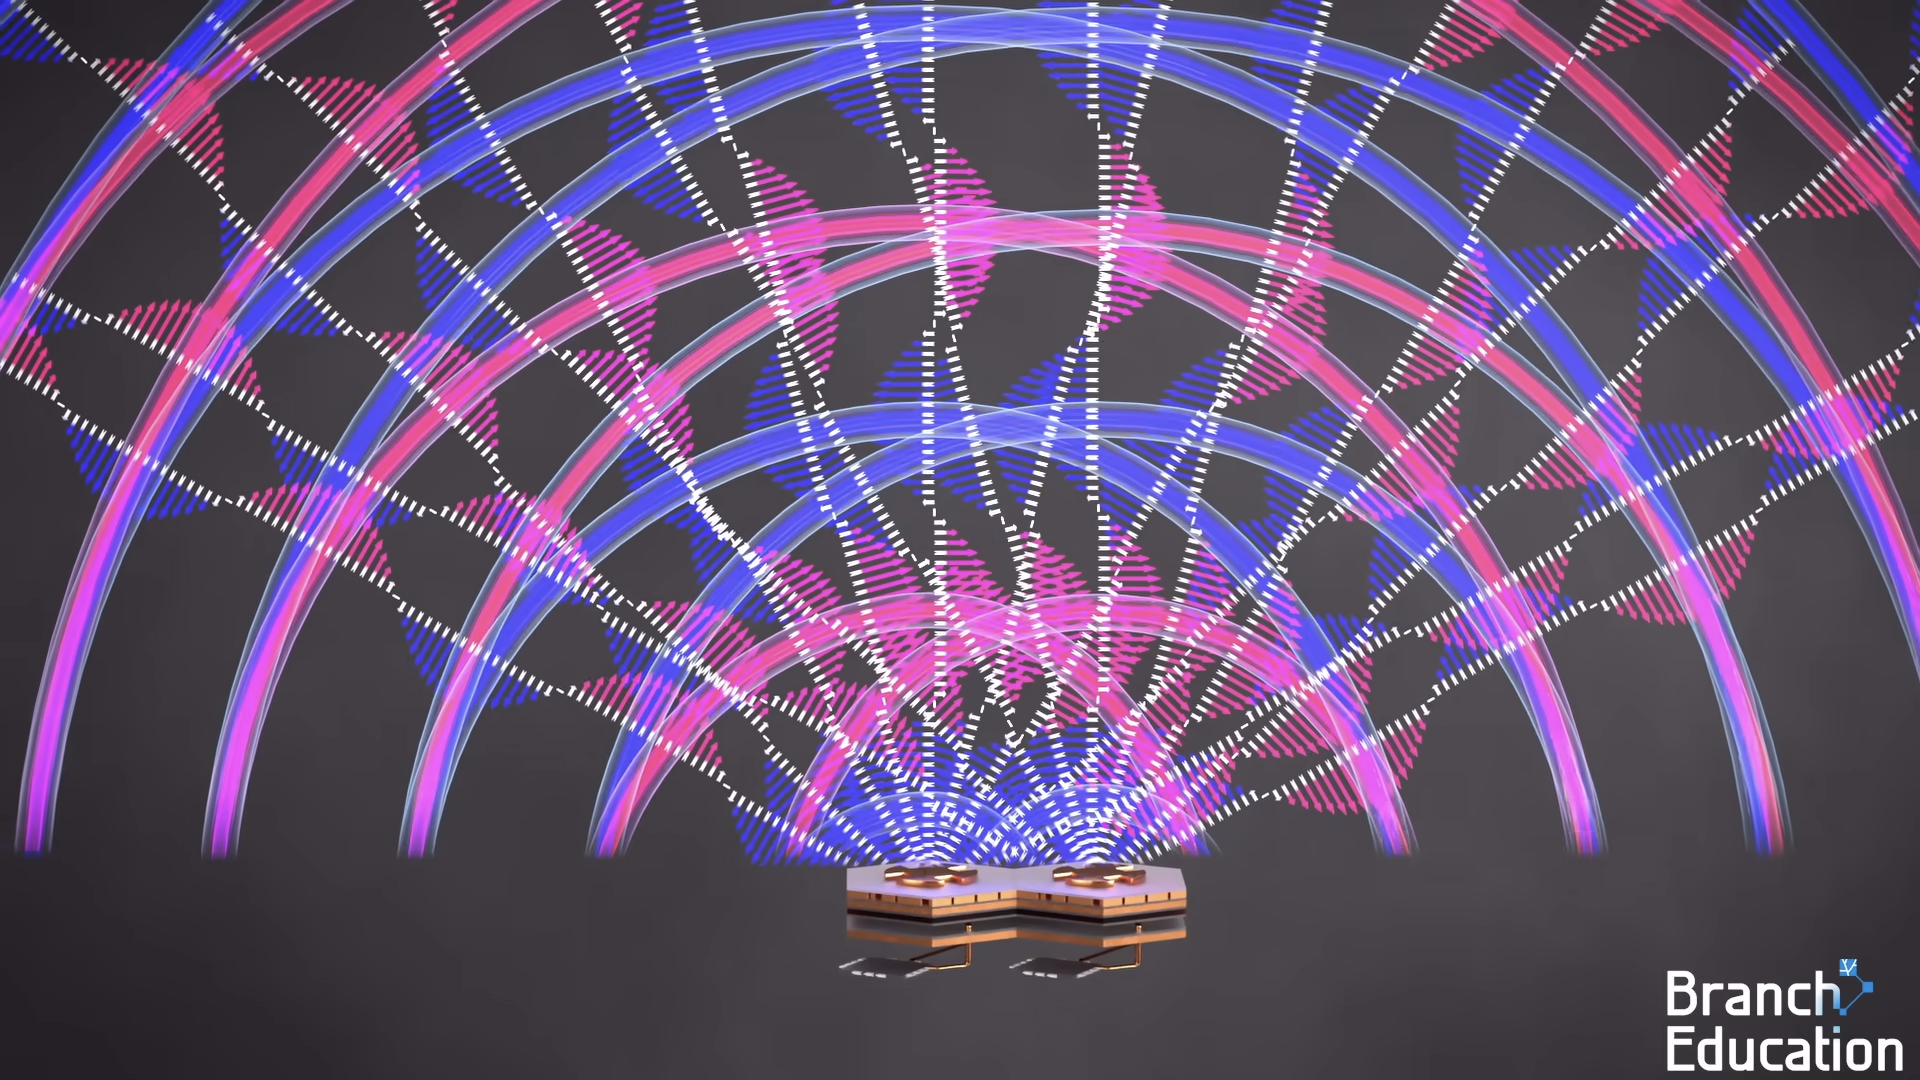
\includegraphics[width=0.8\linewidth]{./res/img/antenna_interference.png}
  \caption{Creazione di interferenze in un array di antenne Aperture Couple Patch \cite{branch_education_how_2022}}
  \label{fig:aperture-couple-patch-antenna-interference}
\end{figure}

Quando aggiungiamo ancora più antenne la zona di interferenza costruttiva diventa ancora più focalizzata rispetto a una singola antenna, in quello che viene chiamato fronte del fascio.
Così, aggiungendo 1280 antenne, possiamo formare un fascio con un'intensità e una direzionalità tali da raggiungere lo spazio \cite{branch_education_how_2022}.

\subsection{Beam Steering: direzionare un fascio di onde elettromagnetiche}
Come menzionato precedentemente dobbiamo direzionare le onde elettromagnetiche per puntare al satellite starlink che viaggia in \ac{LEO} a 27000 km/h.
Usare i motori dell'antenna non è abbastanza preciso e creerebbe stress inutile sui motori.
La soluzione è quindi di usare quello che viene chiamato Phased Array Beam Steering.

Torniamo ancora una volta all'esempio delle due antenne.
Prima stavamo inviando lo stesso segnale alle due antenne, e quindi queste erano in fase l'una con l'altra.
Per fare beam steering invece si invia il segnale alle antenne con una differenza di fase per poterlo angolare.
Come risultato i tempi dei picchi e delle valli emesse da un'antenna sono differenti dalle altre.
In questo modo le posizioni delle interferenze costruttive sono angolati verso una certa direzione, con interferenze distruttive da tutte le altre parti.
Quindi, cambiando continuamente la fase del segnale inviato all'antenna possiamo creare una zona di sweeping di interferenza costruttiva.

Per sapere l'angolo esatto a cui il fascio di onde deve essere indirizzato si usano le coordinate GPS dell'antenna tramite il suo chip GPS, insieme alle posizioni orbitali del satellite Starlink che è conosciuto nel software dell'antenna.
Il software calcola l'angolo e lo shift di fase richiesto per ciascuna delle antenne.
I risultati dei calcoli del phase shift sono successivamente inviati ai 20 chip più grandi chiamati beamformers, e ciascun beamformer coordina 32 chip più piccoli chiamati moduli di front end, ciascuno dei quali controlla 2 antenne.
Ogni pochi microsecondi questi calcoli sono aggiornati e distribuiti in tutto il PCB dell'antenna in modo da orientare perfettamente il segnale verso il satellite.
Come risultato, il raggio può essere orientato ovunque in un campo visivo di 100 gradi \cite{branch_education_how_2022}.
    %!TEX root = ../main.tex

\chapter{Trasmissione dei dati}
\section{Modulazioni utilizzate}
Per inviare i dati al satellite le informazioni sono codificate nelle onde elettromagnetiche attraverso un processo chiamato modulazione.
Il criterio principale per la scelta dello schema di modulazione è basato sulla massimizzazione del data rate e minimizzazione della potenza trasmessa, della larghezza di banda del canale, dell'errore sul simbolo e resistenza alle interferenze.

Le tecniche di modulazione e demodulazione digitale richiedono una maggiore complessità e un elevato livello di integrazione per trasferire grandi quantità di dati e informazioni.
Un filtraggio eccessivo per migliorare l'efficienza spettrale può ridurre le interferenze ma aumentare il \ac{BER} a causa della distorsione dei simboli trasmessi.

Per inviare dati digitali, l'emittente genera un segnale portante a una certa frequenza.
Per codificare il segnale digitale nella sinusoide sono poi utilizzate le seguenti tecniche:
\begin{itemize}
  \item Amplitude-shift modulation (keying): varia l'ampiezza del segnale (cioè la tensione).
  \item Frequency-shift modulation: due (o più) frequenze vicine alla frequenza portante sono utilizzate.
  \item Phase-shift modulation: varia la fase della portante a intervalli spaziati del periodo di simbolo.
\end{itemize}

Oltre alla modulazione i dati vengono trasmessi utilizzando anche tecniche di multiplexing.
Il multiplexing consente di combinare più segnali in un singolo canale di trasmissione, massimizzando l'uso della banda e migliorando l'efficienza del sistema.
Esistono due principali approcci al multiplexing: FDM (Frequency Division Multiplexing) e TDM (Time Division Multiplexing).
L'FDM suddivide lo spettro di frequenza in sottocanali, dando a ciascun utente l'utilizzo esclusivo di un sottocanale.
Un problema con FDM è che a un utente è data tutta la sottobanda, e se non ha dati da inviare la banda è sprecata, dato che non può essere utilizzata da un altro utente.
Il TDM invece utilizza il time slicing per dare a ciascun utente l'intera banda, ma solo per una frazione di tempo alla volta.
Di nuovo, se l'utente non ha dati da inviare durante il suo timeslice, la banda non è utilizzata, e quindi è sprecata.

La capacità di un satellite Starlink sarà di 20 Gbit/s quando opererà in due polarizzazioni con modulazione 64-\ac{QAM}.
Ad oggi la rete può usare solo una polarizzazione.

Per lavorare con la 64-\ac{QAM} è necessario avere un \ac{SNR} di più di 17 dB, infatti in questo caso il \ac{BER} sarebbe $0.49 \%$.
Questo perchè per una M-\ac{QAM} $P_e \approxeq 4 (1-\frac{1}{sqrt{M}}) Q(\sqrt{\frac{3}{M - 1} \frac{E_s}{N_0}})$ con $\frac{E_s}{N_0}$ che è il SNR.
Dalla probabilità di errore sul simbolo possiamo calcolare $P_{\text{bit}} \approxeq \frac{P_e}{\log_2 M}$ per $\frac{E_s}{N_0} >> 1$.

Al momento questo parametro al terminale UT-1 è tra gli 11 e i 12.5 dB, che permette l'uso di una 16-32\acs{APSK} e ha un'efficienza spettrale di 4.5 bit/s/Hz al massimo.

Considerando anche l'applicazione di un codice di canale, 
caratterizzato da un code-rate $\frac{k}{n}$ ($k$ bit di informazione ogni $n$ bit di codice), le efficienze spettrali che si che si ottengono con diverse combinazioni di modulazione e code-rate sono illustrate in tabella \ref{tab:spectral-efficiency}

\begin{table}[h]
\centering
\begin{tabular}{|c|c|c|c|}
\hline
\textbf{Modulation} & \textbf{Code rate} & \makecell{\textbf{Spectral efficiency}\\ \textbf{bit/s/Hz}} \\ \hline
QPSK     & 0.5   & 0.989  \\ \hline
8PSK     & 0.75  & 2.228  \\ \hline
8PSK     & 0.833 & 2.479  \\ \hline
16APSK   & 0.666 & 2.637  \\ \hline
16APSK   & 0.75  & 2.967  \\ \hline
32APSK   & 0.9   & 4.453  \\ \hline
64QAM    & 0.772 & 4.5234 \\ \hline
64QAM    & 0.873 & 5.1152 \\ \hline
64QAM    & 0.948 & 5.5547 \\ \hline
\end{tabular}
\caption{Efficienza spettrale di Starlink \cite{rozenvasser_estimation_2023}}
\label{tab:spectral-efficiency}
\end{table}

\paragraph{Link budget}
La potenza ricevuta al terminale utente è data da:
\begin{equation}
P_{rx} = P_{tx} + G_{tx} + G_{rx} - L_{tx} - L_{rx} - L_{atm} - L_{p}
\label{eq:received-power}
\end{equation}

In questa equazione, $P_{tx}$ è la potenza del trasmettitore, $G_{tx}$ e $G_{rx}$ sono i guadagni del trasmettitore e del ricevitore, $L_{tx}$ e $L_{rx}$ sono le perdite ai trasmettitori e ricevitori, $L_{atm}$ è la perdita atmosferica, e $L_{p}$ è il path loss introdotto dalla separazione tra il trasmettitore e il ricevitore.

La perdita atmosferica $L_{atm}$ è dipendente dalla banda di frequenza e pressione atmosferica $P_{atm}$.
Per la Ku/Ka-band $L_{atm} = 0.97 dB/km$ in media.

\begin{figure}[htbp]
  \centering
  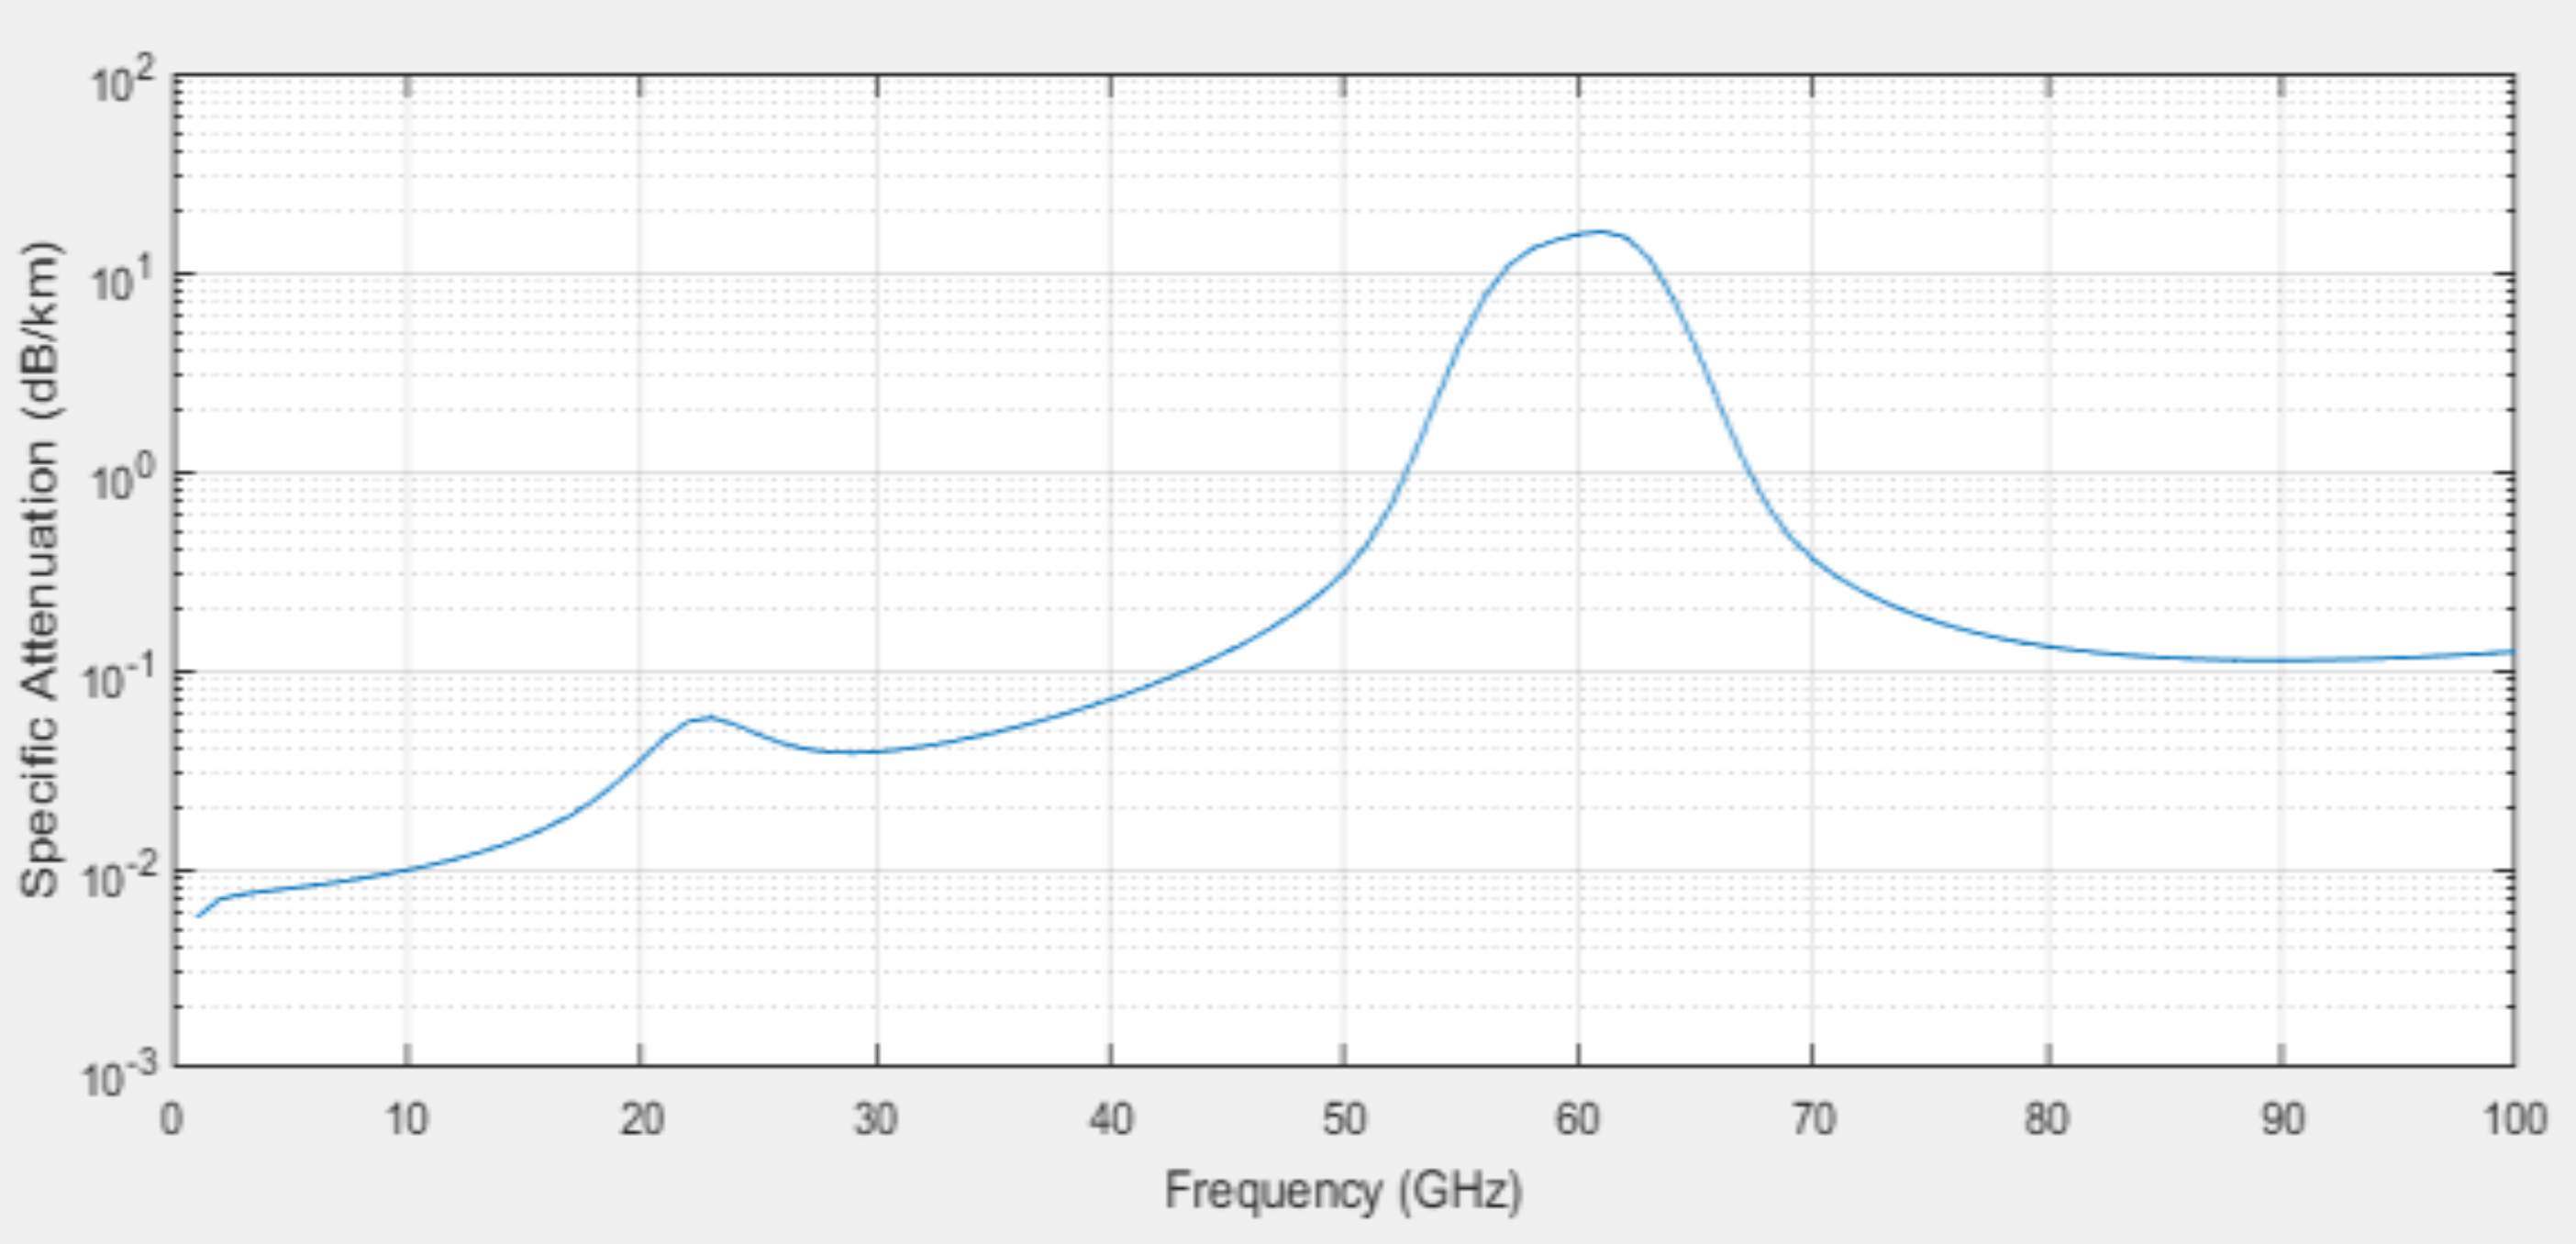
\includegraphics[width=0.8\linewidth]{./res/img/atmospheric_losses_simulation.png}
  \caption{Perdite atmosferiche.}
  \label{fig:atmospheric-losses-simulation}
\end{figure}

Osserviamo in figura \ref{fig:atmospheric-losses-simulation} un picco del parametro $L_{atm}$ a 60 GHz.
Per ridurre l'influenza delle perdite atmosferiche è preferibile usare i range di frequenza fino a 53 GHz, che corrisponde al piano di frequenze proposto da SpaceX (tabella \ref{tab:starlink-frequency-allocation-modulation-type}).
Per la trasmissione in uplink si usano le frequenze 14-52.4 GHz e per la trasmissione in downlink le frequenze 10.7-42.5 GHz.
Nella tabella \ref{tab:starlink-frequency-allocation-modulation-type} possiamo anche vedere i tipi di modulazione.
Il tipo di modulazione può cambiare da \ac{BPSK} a 64-\ac{QAM}.

Esiste un trade-off tra la semplicità al ricevitore di un segnale facilmente demodulabile e l'efficienza di modulazione di quel segnale.
Due delle efficienze di maggior interesse nei sistemi di comunicazione satellitari sono l'efficienza spettrale e l'efficienza energetica.

\paragraph{Efficienza spettrale}
L'efficienza spettrale si riferisce al rapporto tra la velocità dei dati e la larghezza di banda del segnale, che misura quanti bit al secondo possono essere trasmessi per Hertz di larghezza di banda (bps/Hz).
Secondo il teorema della larghezza di banda minima di Nyquist, è possibile trasmettere fino a 2 bps/Hz in banda base senza codifica.
I sistemi ibridi fase-ampiezza a più livelli o sistemi M-ari possono raggiungere efficienze spettrali ancora più elevate a costo di una maggiore complessità. Tuttavia, bisogna comunque tenere presente che la velocità massima dei dati senza errori di questi sistemi è in ultima analisi limitata dal rapporto segnale/rumore (\ac{SNR}), come descritto dal teorema della capacità del canale di Shannon \cite{don_k_lefevre_power-efficient_1989}.

\paragraph{Efficienza energetica}
L'efficienza energetica è il rapporto tra la velocità dei dati e la potenza necessaria per trasmettere i dati senza errori.
Nei sistemi reali, la potenza richiesta dipende anche da fattori quali le figure di rumore, i guadagni dell'antenna e la distanza tra trasmettitore e ricevitore.
Per effettuare confronti relativi, un metodo semplice consiste nel confrontare l'\ac{SNR} richiesto per ottenere lo stesso tasso di errore di bit (\ac{BER}).
Questo approccio consente di confrontare sistemi che sono identici in termini di figura di rumore, perdita di percorso e altri fattori ma differiscono nella modulazione.
La differenza nell'SNR richiesto rivela le prestazioni relative di ciascun tipo di modulazione \cite{don_k_lefevre_power-efficient_1989}.

\begin{table}[h]
\centering
\begin{tabular}{|c|c|c|}
\hline
\textbf{Caratteristica} & \textbf{Uplink} & \textbf{Downlink} \\ \hline
Frequenza (GHz)  & \makecell{14.0-14.5 \\ 27.5-29.1 \\ 29.5-30.0 \\ 47.2-52.4}  & \makecell{10.7-12.7\\17.8-18.6\\18.8-19.3\\37.5-42.5} \\ \hline
Tipo di modulazione  & \makecell{\acs{BPSK},\\M\acs{QAM}} & \makecell{\acs{OQPSK},\\ M\acs{QAM}} \\ \hline
\end{tabular}
\caption{Schemi di modulazione \cite{rozenvasser_estimation_2023}.}
\label{tab:starlink-frequency-allocation-modulation-type}
\end{table}

% $L_p = 20 \log_{10} (\frac{4 \pi d}{\lambda})$

\begin{figure}[htbp]
  \centering
  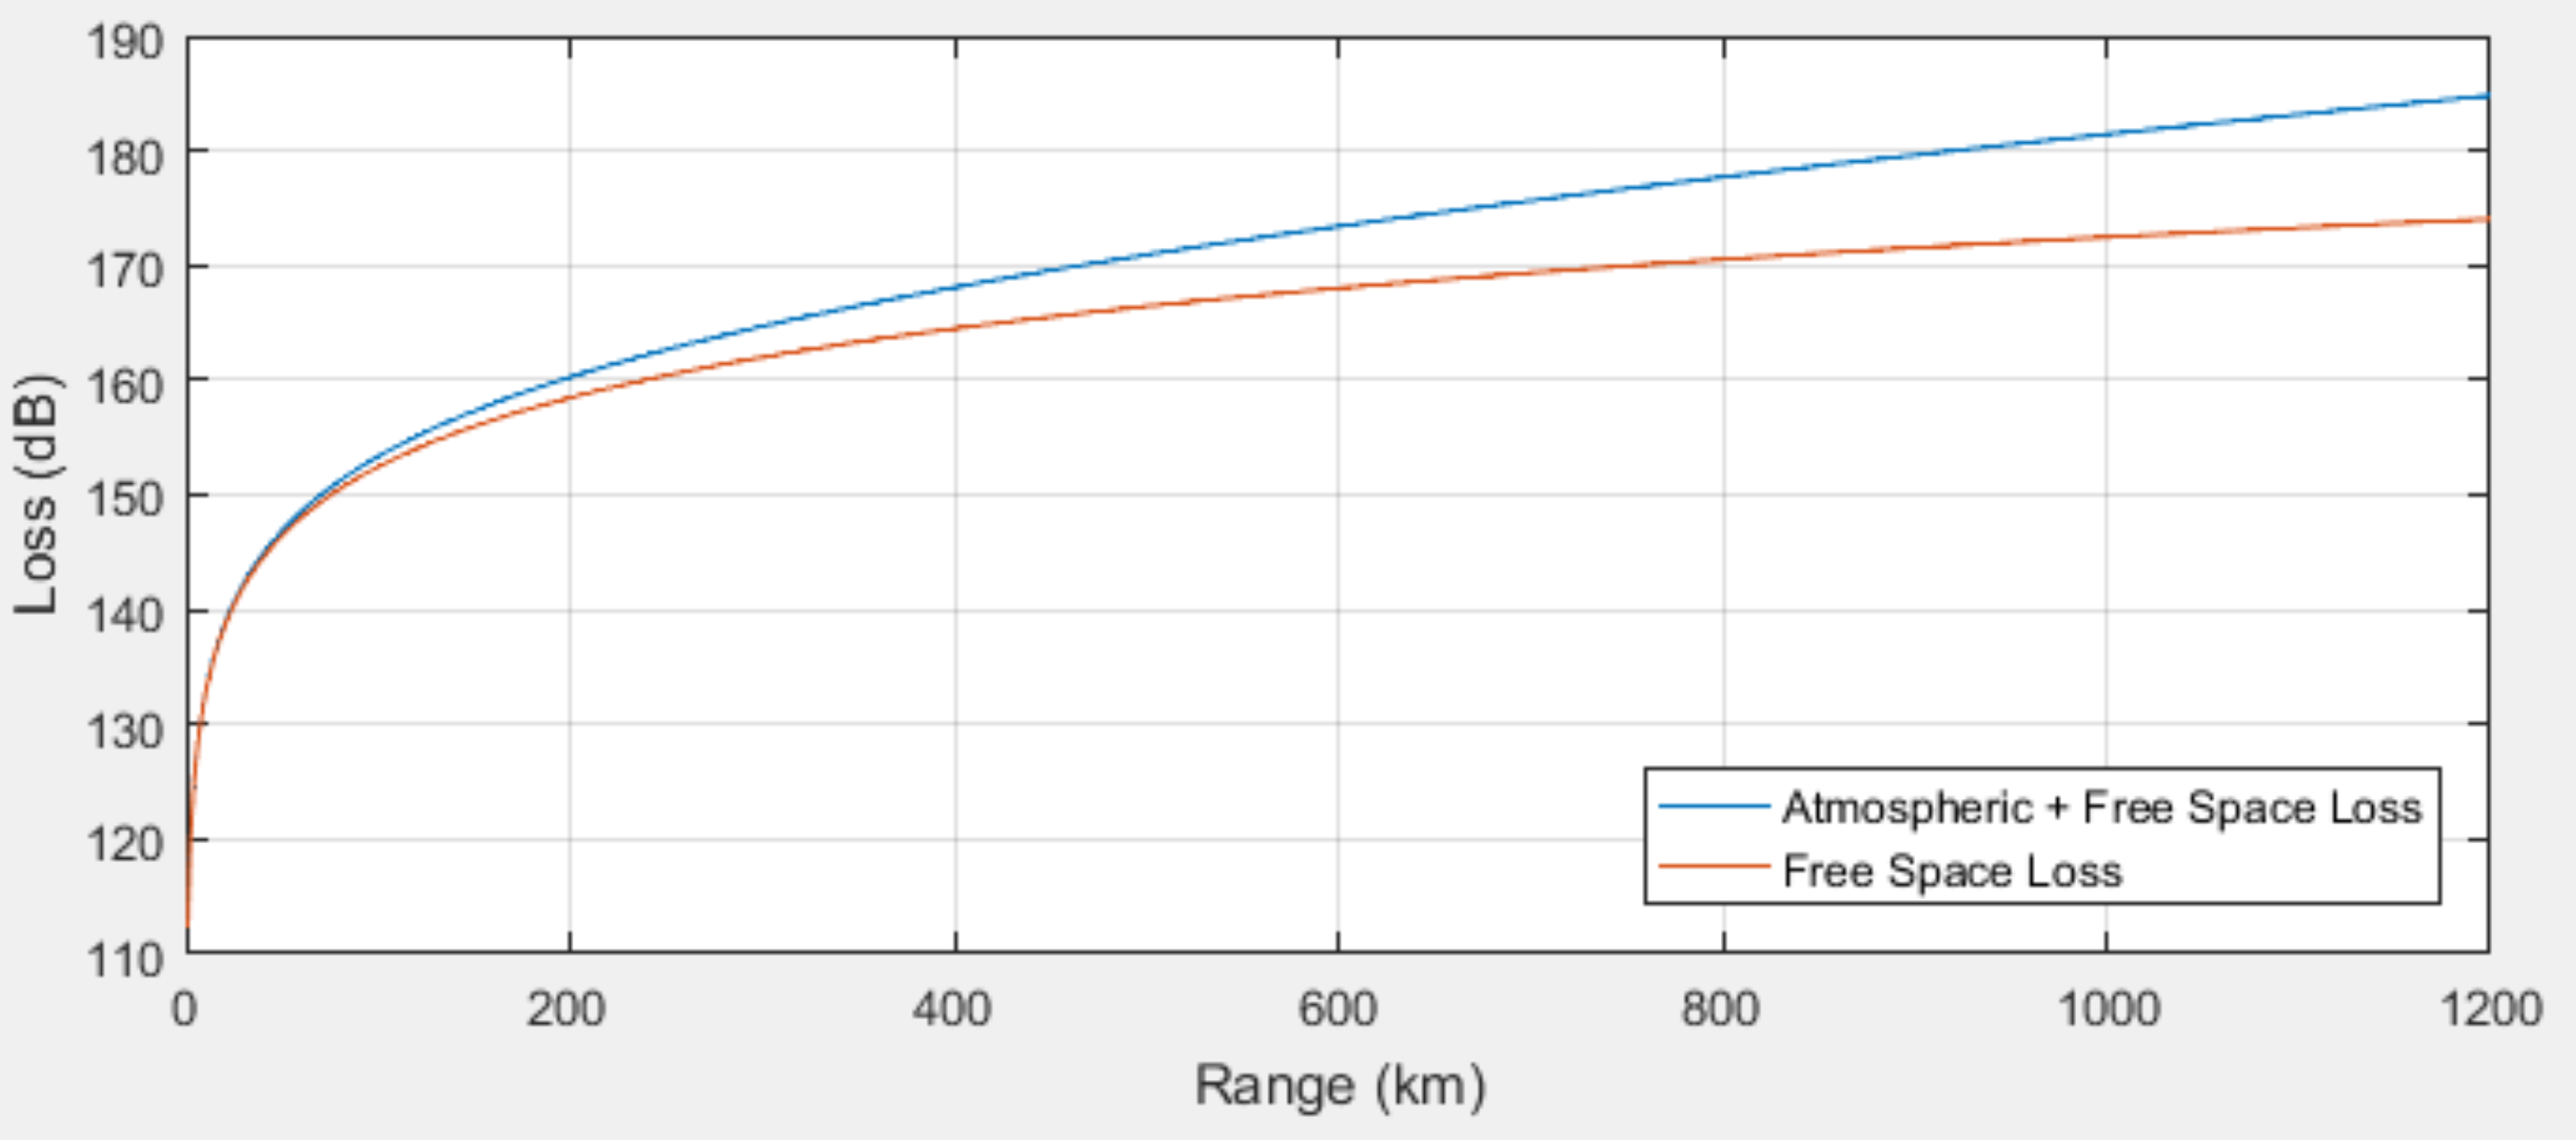
\includegraphics[width=0.8\linewidth]{./res/img/free_space_path_loss_atm_loss.png}
  \caption{Path loss ($L_p$) nello spazio libero e perdita atmosferica.}
  \label{fig:free-space-path-loss-atm-loss}
\end{figure}

Il path loss nello spazio libero è il contributore principale alla perdita di potenza come si vede in figura \ref{fig:free-space-path-loss-atm-loss}.
Alle altitudini calcolate per i satelliti Starlink, questo valore è di 160-175 dB.
La perdita totale dal path loss nello spazio libero e le perdite atmosferiche sono 165-185 dB.

I risultati della modellazione e del calcolo della dipendenza della potenza ricevuta dal terminale utente dall'altezza dell'orbita del satellite per varie frequenze (da 10 a 50 GHz) sono illustrati nella figura \ref{fig:link-budget-wo-ecc}.

\begin{figure}[htbp]
  \centering
  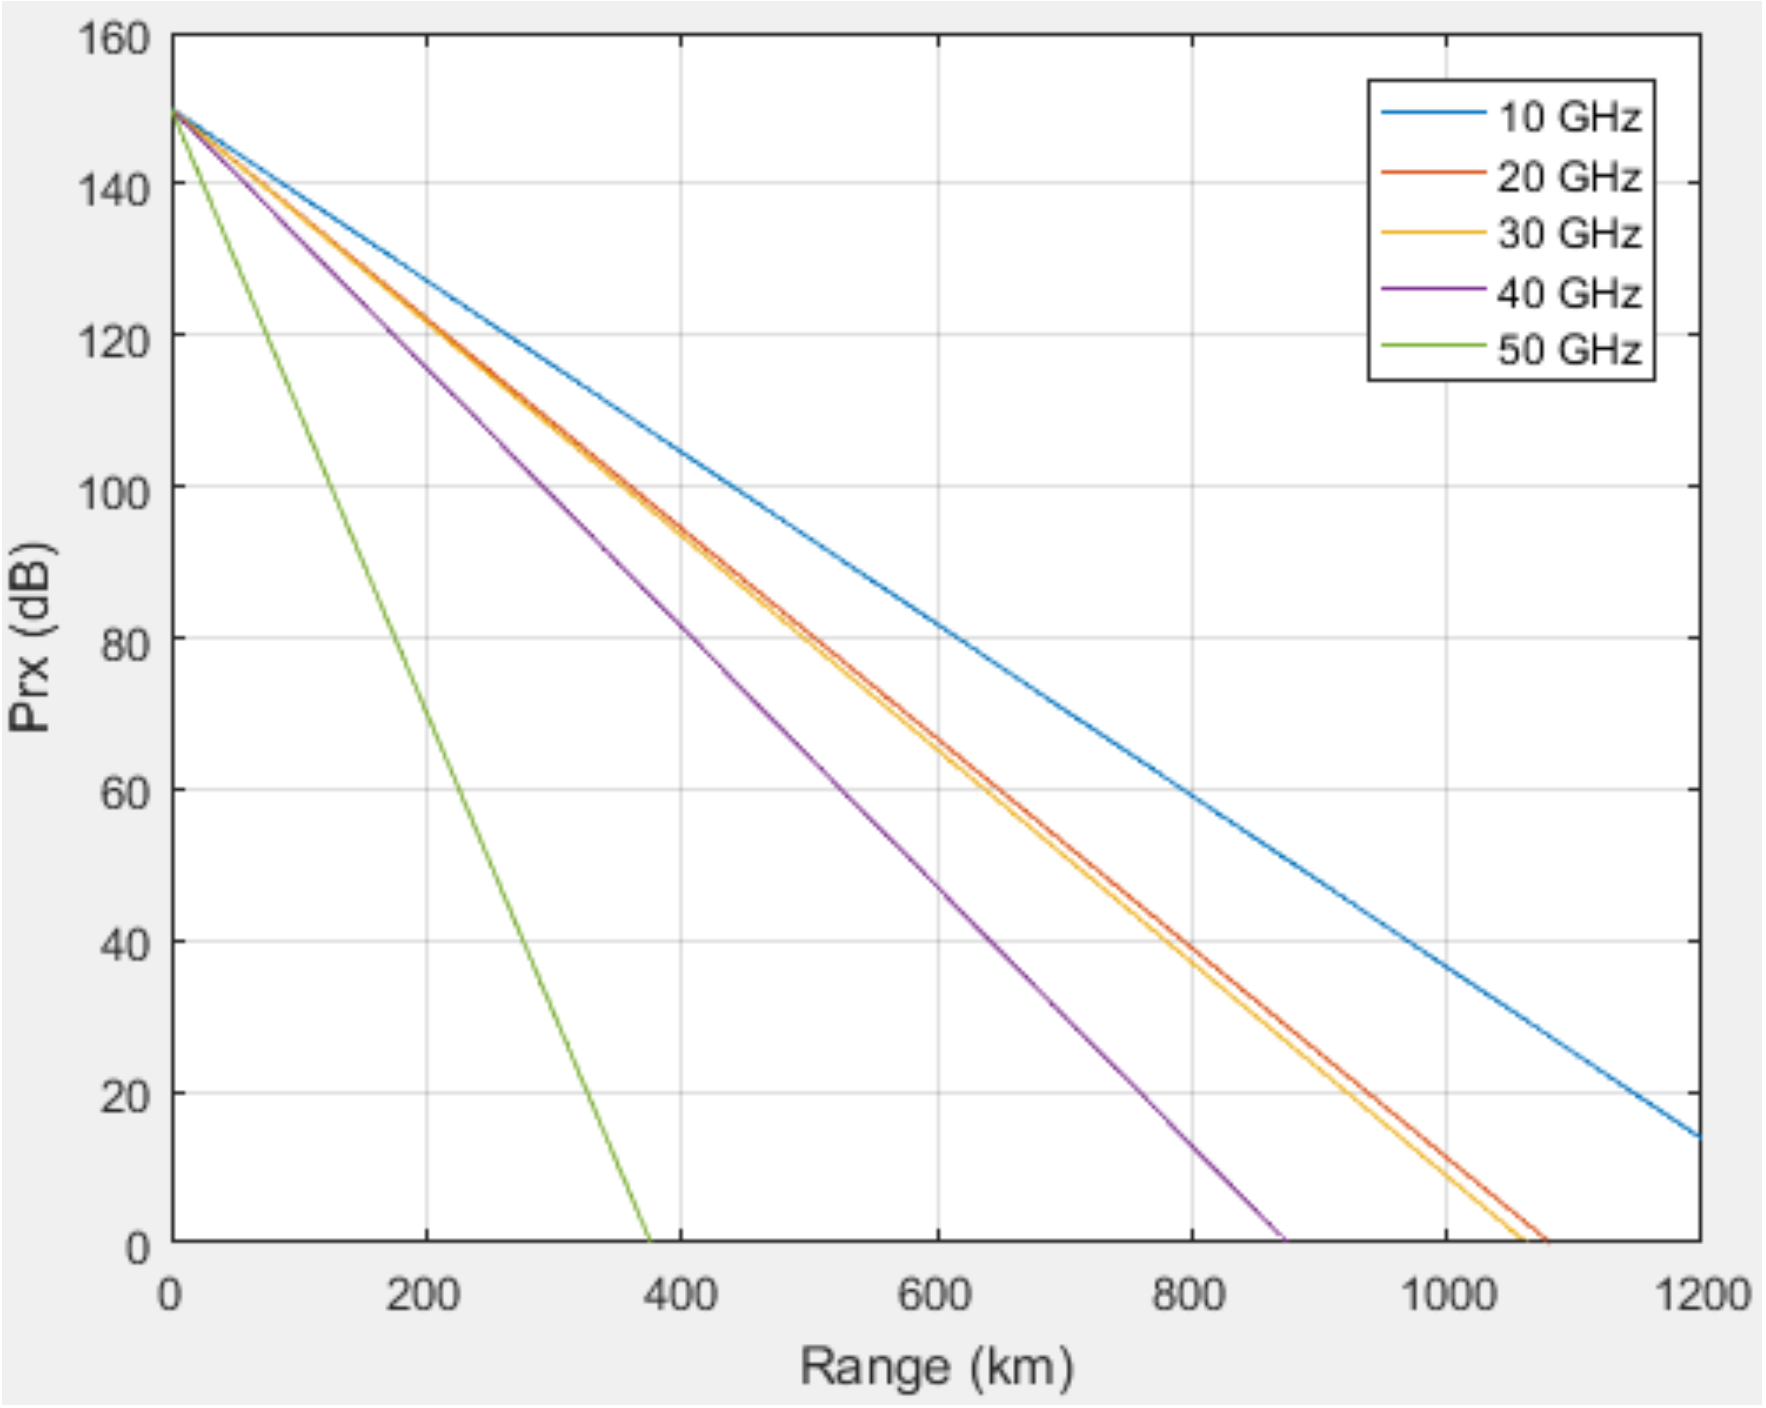
\includegraphics[width=0.8\linewidth]{./res/img/link_budget_wo_ecc.png}
  \caption{Link budget senza \ac{ECC}.}
  \label{fig:link-budget-wo-ecc}
\end{figure}

Dalla figura \ref{fig:link-budget-wo-ecc} si può vedere che il valore più alto della potenza del segnale è 150 dBW.
Finchè il segnale passa attraverso l'atmosfera gradualmente viene attenuato.
L'attenuazione avviene anche sui dispositivi ricevitori e trasmettitori.
Il grado di attenuazione dipende da molti parametri e limita l'altezza dell'orbita del satellite.

È consuetudine utilizzare un codice a correzione di errore per aumentare l'immunità al rumore dei sistemi.
In questo caso, utilizziamo un codice a correzione di errore per aumentare il link budget.

Aggiungiamo CG, guadagno di codifica dovuto al codice a correzione d'errore (\ac{ECC}), all'equazione (\ref{eq:received-power}) che diventa quindi:

\begin{equation}
  P_{rx} = P_{tx} + G_{tx} + G_{rx} - L_{tx} - L_{rx} - L_{atm} - L_{p} + CG
\end{equation}

I risultati della modellazione e calcolo della dipendenza della potenza ricevuta al terminale utente all'altezza dell'orbita del satellite per frequenze diverse (dai 10 ai 50 GHz), considerando l'uso di un codice di correzione di errore con un guadagno di codice di 10 dB sono mostrate in figura \ref{fig:link-budget-w-ecc}.

\begin{figure}[htbp]
  \centering
  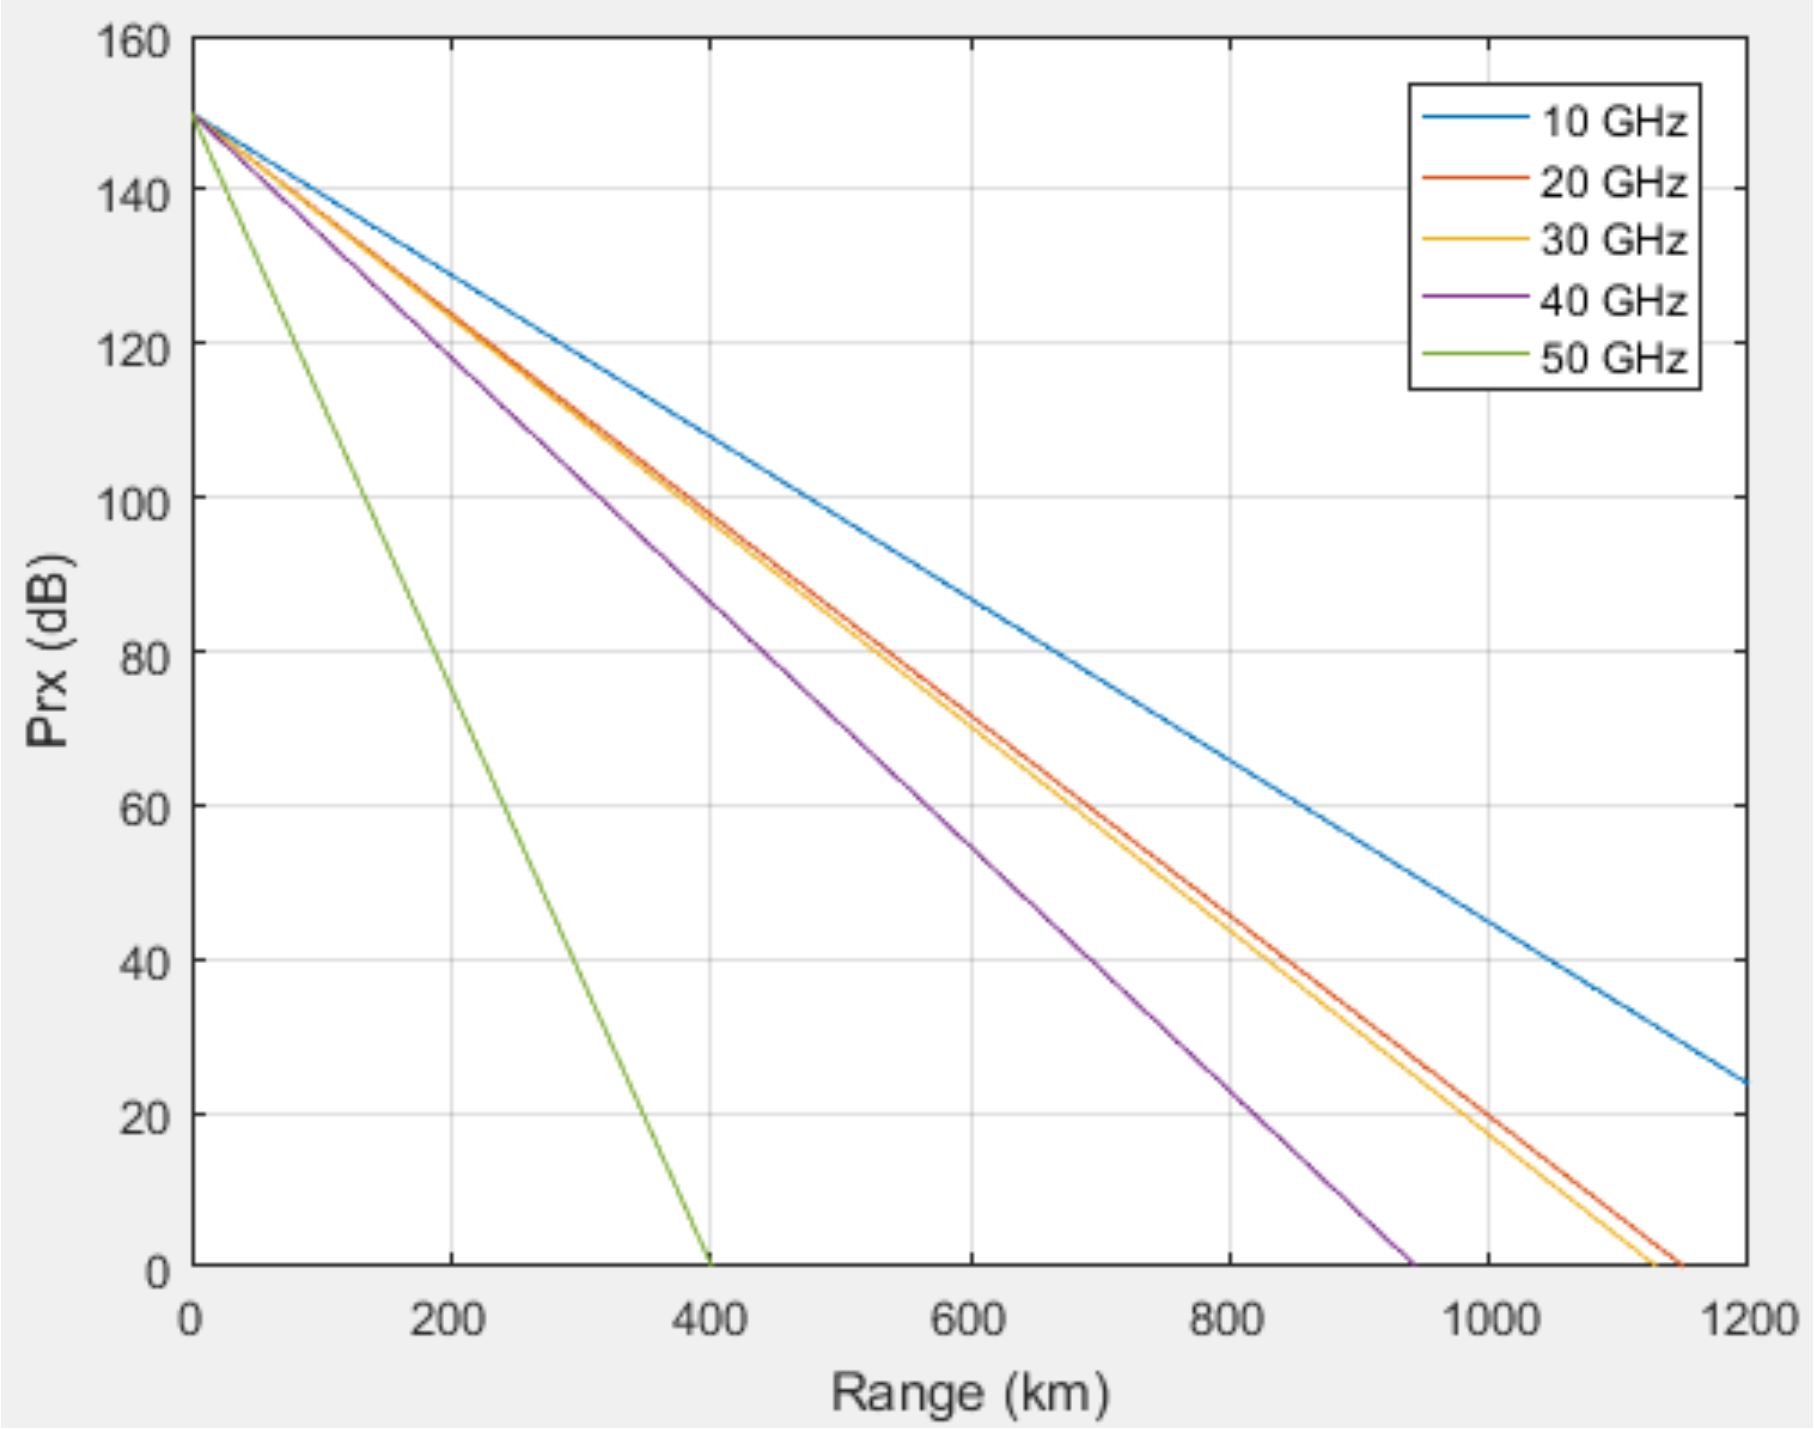
\includegraphics[width=0.8\linewidth]{./res/img/link_budget_w_ecc.png}
  \caption{Link budget con \ac{ECC}.}
  \label{fig:link-budget-w-ecc}
\end{figure}

Per assicurare la minima probabilità d'errore è necessario avere un margine del \ac{SNR} al ricevitore, che dipende dal tipo di modulazione.
Dalla figura \ref{fig:link-budget-w-ecc} possiamo vedere che ad alte frequenze l'altezza dell'orbita è limitata a 340 km.
Il lancio della maggior parte dei satelliti è pianificata a quest'altezza.
Per frequenze più basse, possono essere utilizzate orbite più alte a 550 km e 1110 km \cite{rozenvasser_estimation_2023}.

\subsection{Binary Phase Shift Keying (BPSK)}
\ac{BPSK} è la forma più semplice di phase shift keying (\ac{PSK}).
Utilizza due fasi, che sono separate da 180$\degree$ e quindi può essere anche chiamata 2-\ac{PSK}.
Non importa particolarmente dove i punti sono posizionati nella costellazione, e in figura \ref{fig:bpsk-diagram} sono posizionati sull'asse dei reali, rispettivamente a 0$\degree$ e 180$\degree$.
La costellazione è la più robusta di tutte le \ac{PSK}, ma può solo modulare 1 bit/simbolo e non è quindi adatta per applicazioni ad alta velocità di trasmissione dati.

\begin{figure}[htbp]
  \centering
  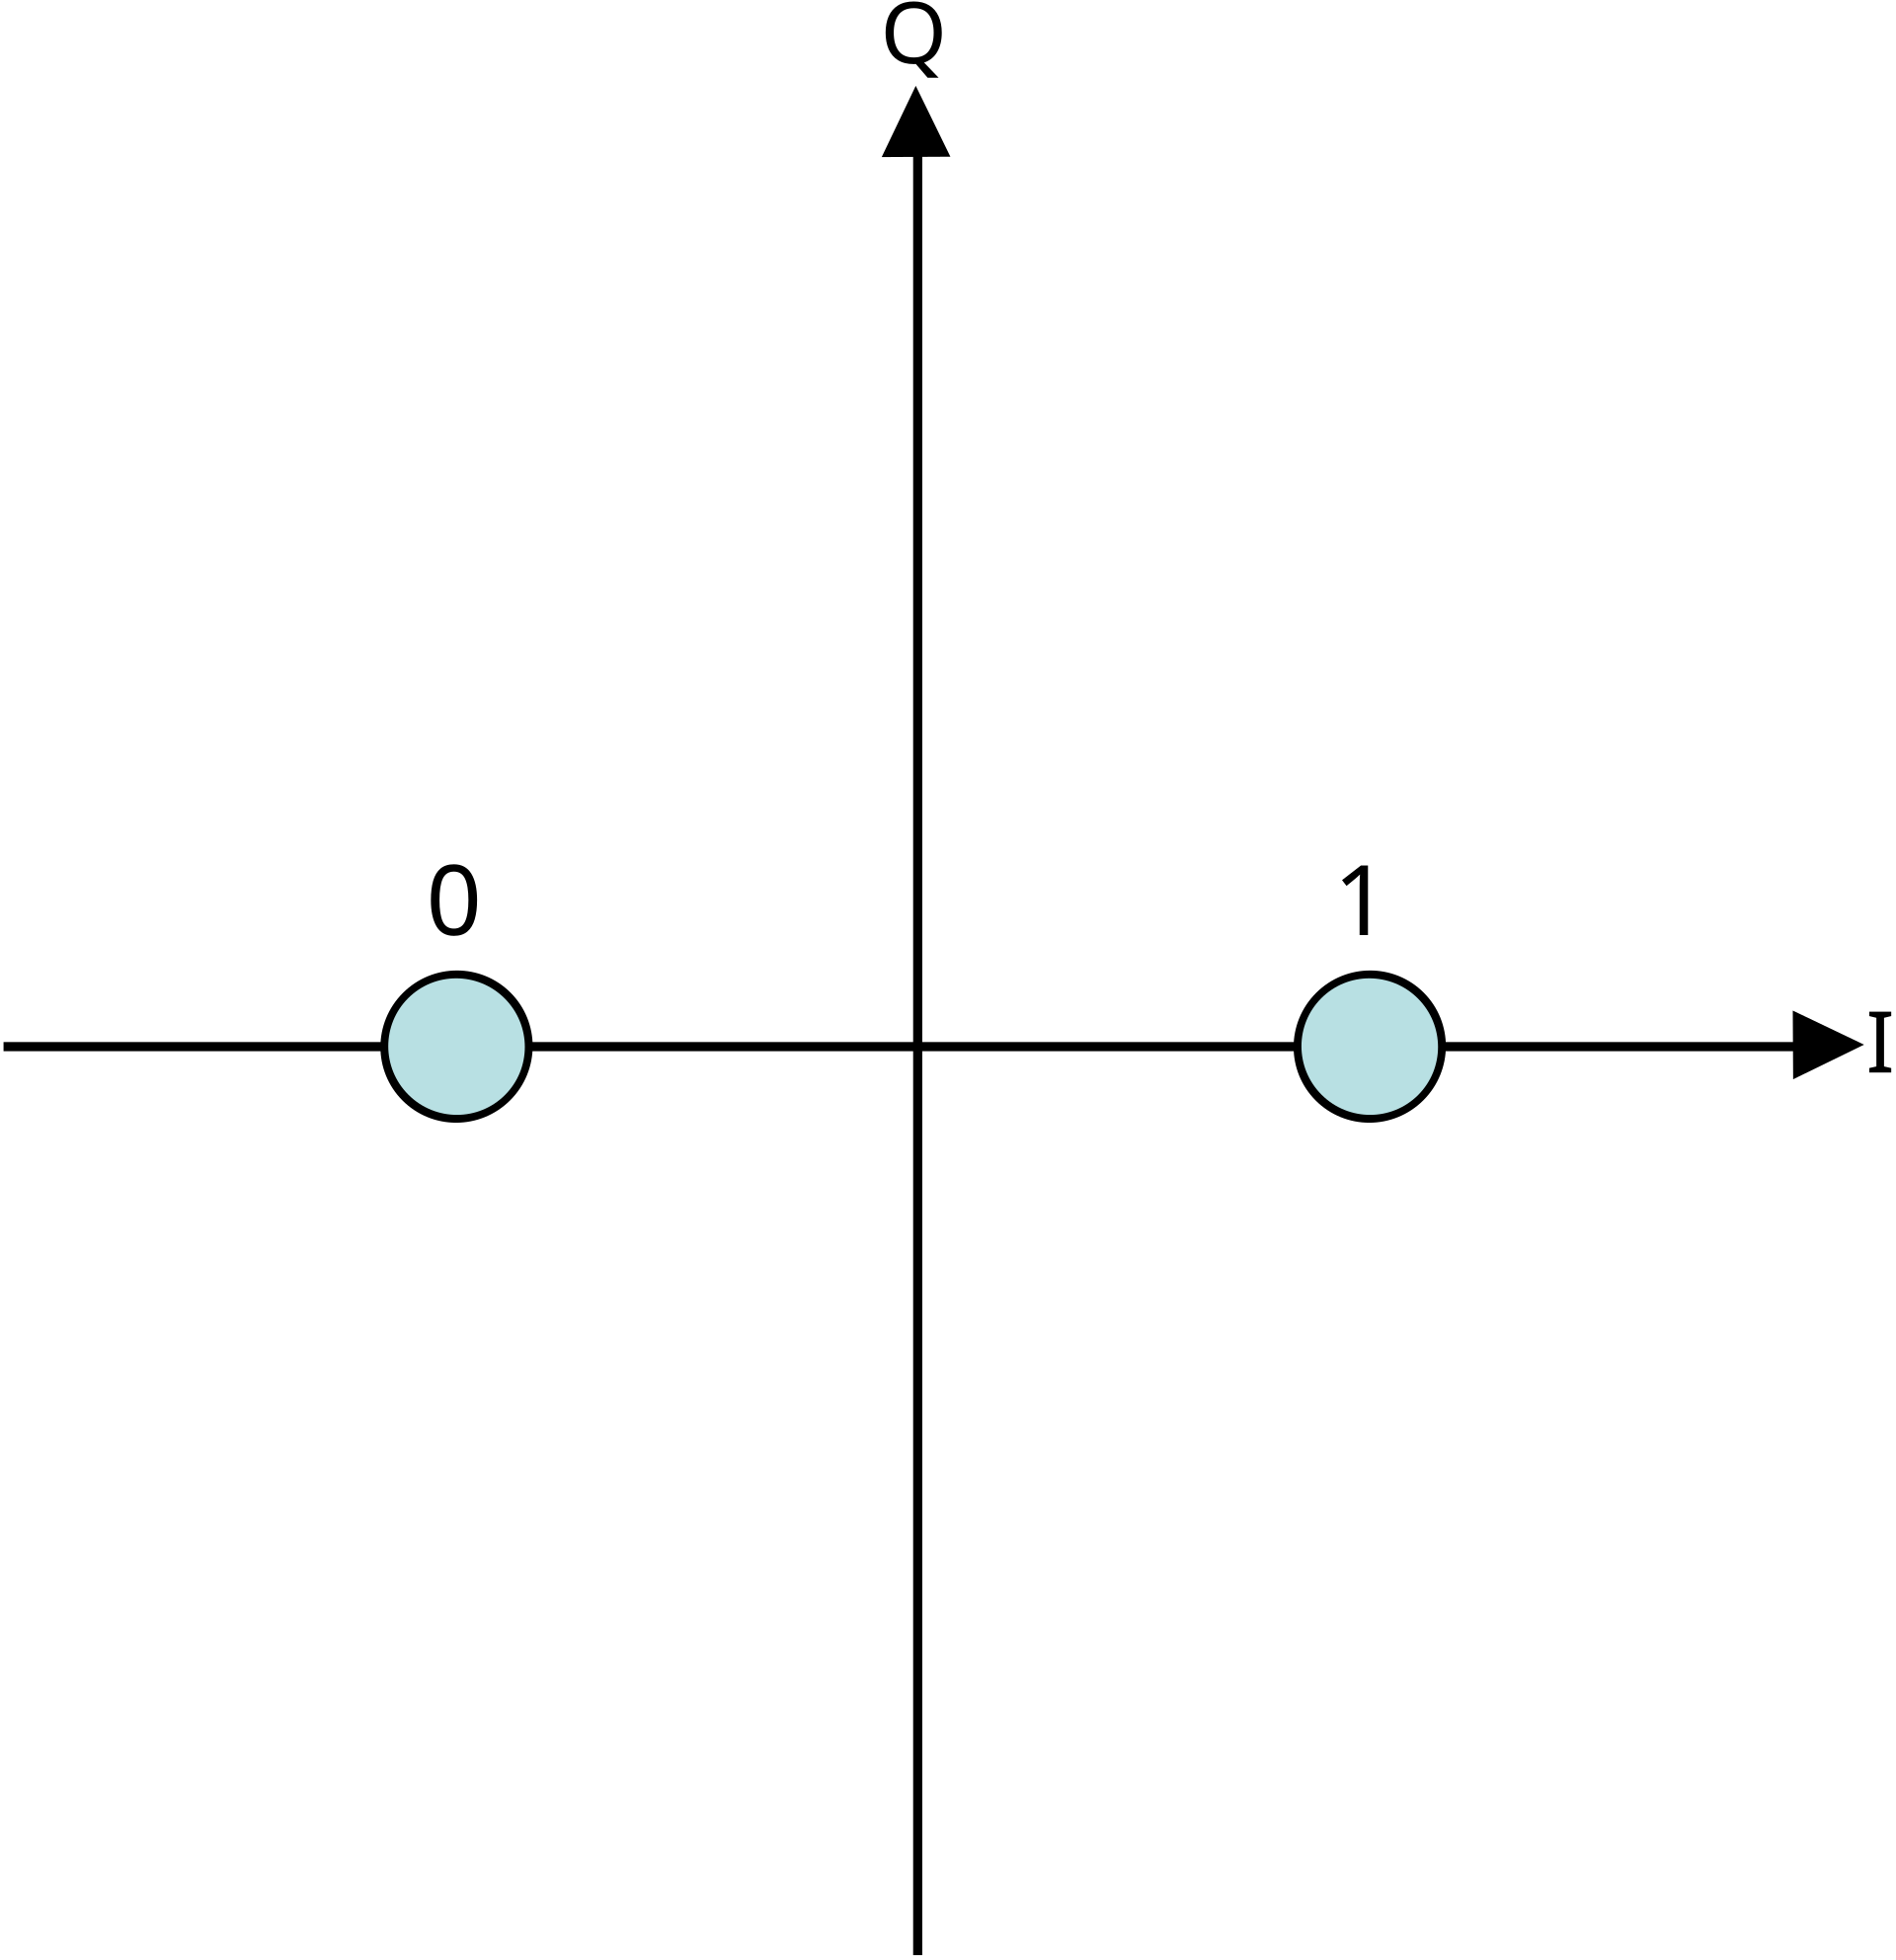
\includegraphics[width=0.4\linewidth]{./res/img/bpsk_diagram.png}
  \caption{Diagramma per la costellazione BPSK.}
  \label{fig:bpsk-diagram}
\end{figure}

La forma generale per la \ac{BPSK} segue l'equazione:
$$s_n(t) = \sqrt{\frac{2E_b}{T_b}} \cos(2\pi f t + \pi(1-n)) \quad , n = 0,1 $$
Questo dà due fasi: 0 e $\pi$.

Dove $E_b$ è l'energia per bit, $\frac{N_0}{2}$ la densità spettrale del rumore e $T_b$ il periodo di bit.

Il bit error rate (\ac{BER}) della \ac{BPSK} sotto ipotesi di rumore addittivo Gaussiano bianco (\acs{AWGN}) può essere calcolata come:
$$P_b = Q(\sqrt{\frac{2 E_b}{N_0}})$$

\subsection{Quadrature Phase Shift Keying (QPSK)}
A volte viene chiamata anche 4-\ac{PSK}, o 4-\ac{QAM} (anche se i concetti alla base sono diversi le onde radio risultanti sono esattamente le stesse).
La \ac{QPSK} utilizza quattro punti sul diagramma delle costellazioni, equispaziate attorno a un cerchio.
Con quattro fasi, \ac{QPSK} può codificare due bit per simbolo, utilizzando la codifica di Gray per minimizzare il bit error rate (\ac{BER}).

Si può anche utilizzare una \ac{QPSK} per raddoppiare il data rate rispetto a una \ac{BPSK} utilizzando la stessa banda, oppure per mantenere lo stesso data rate di una \ac{BPSK} ma dimezzando la banda richiesta.
Nel secondo caso, il \ac{BER} di una \ac{QPSK} è esattamente lo stesso \ac{BER} di una \ac{BPSK}.

\begin{figure}[htbp]
  \centering
  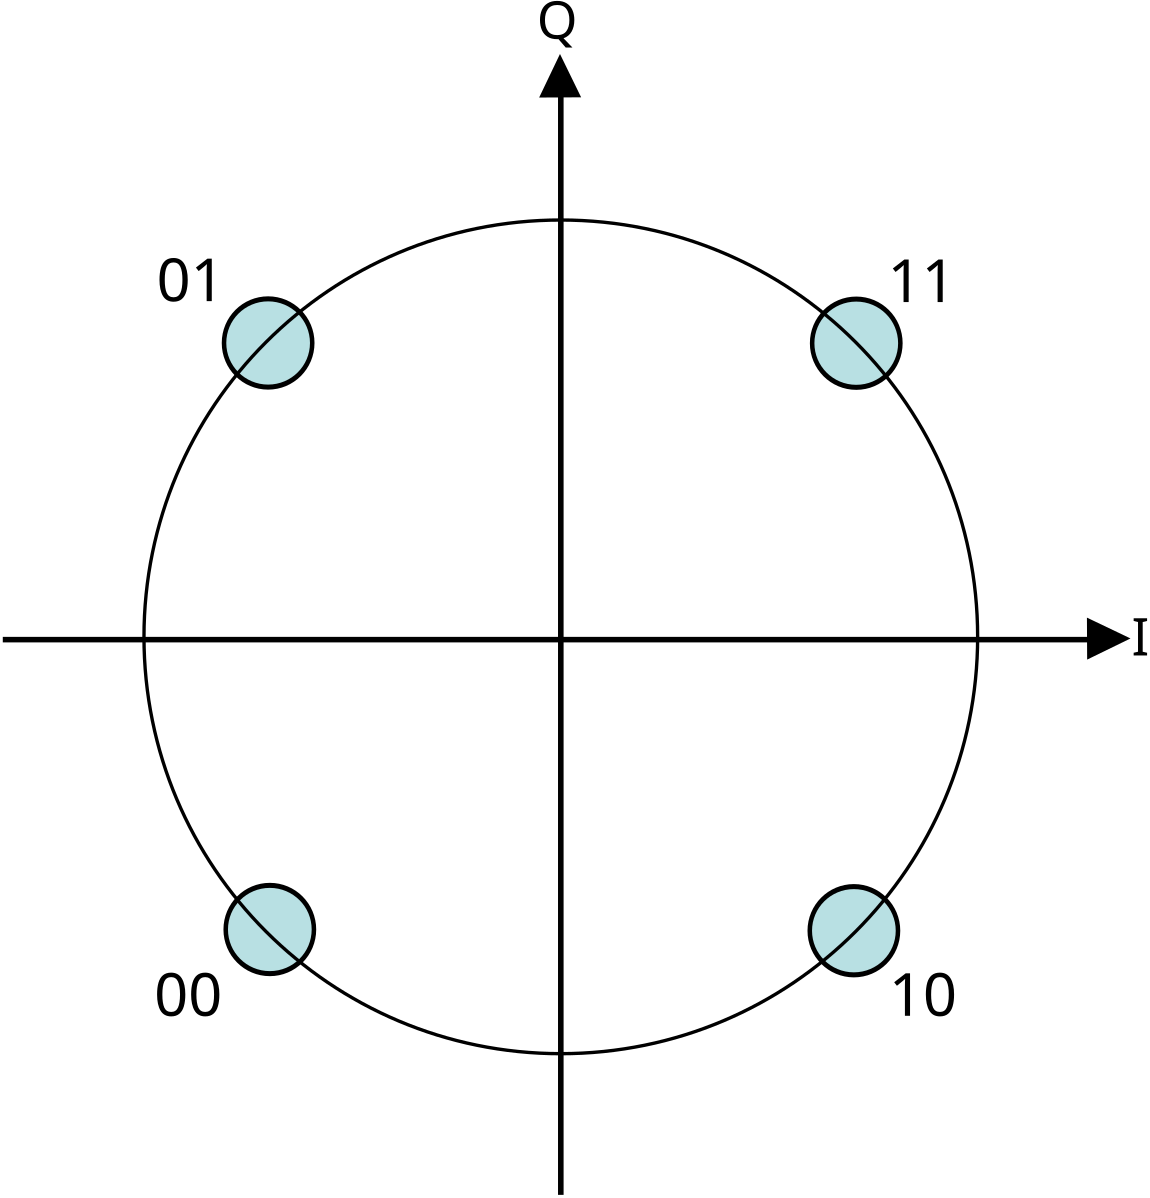
\includegraphics[width=0.4\linewidth]{./res/img/qpsk_diagram.png}
  \caption{Diagramma per la costellazione QPSK.}
  \label{fig:qpsk-diagram}
\end{figure}

L'implementazione di una \ac{QPSK} è più generale di quella di una \ac{BPSK}.
L'equazione dei segnali della costellazione è:
$$s_n(t) = \sqrt{\frac{2 E_s}{T_s}} \cos(2 \pi f_c t + (2n - 1)\frac{\pi}{4}) \quad , n=1,2,3,4$$

Dove $E_s$ è l'energia e $T_s$ il periodo di simbolo.

Da questa formula otteniamo le fasi: $\frac{\pi}{4},\frac{3\pi}{4},\frac{5\pi}{4},\frac{7\pi}{4}$.

Questo risulta in un segnale bidimensionale con base ortonormale: $$\phi_1(t) = \sqrt{\frac{2}{T_s}} \cos(2 \pi f_c t) \quad, \phi_2(t) = \sqrt{\frac{2}{T_s}} \sin(2 \pi f_c t)$$.
La prima componente della base viene utilizzata come componente in fase del segnale, e la seconda componente come quadratura.
Quindi, i segnali della costellazione corrispondono ai 4 punti $(\pm \sqrt{\frac{E_s}{2}}, \pm \sqrt{\frac{E_s}{2}})$.
I fattori di $\frac{1}{2}$ indicano che la potenza totale è distribuita equamente tra le due portanti.

Confrontando i segnali della base con quelli della \ac{BPSK} si vede che la \ac{QPSK} può essere vista come due segnali \ac{BPSK} indipendenti.

Anche se la \ac{QPSK} può essere vista come una modulazione quaternaria, è più semplice vederla come due portanti in quadratura modulate indipendentemente.
Con questa interpretazione, i bit pari (o dispari) vengono utilizzati per modulare la componente in fase della portante, mentre i bit dispari (o pari) vengono utilizzati per modulare la componente in quadratura-fase della portante.
\ac{BPSK} viene utilizzato su entrambe le portanti e possono essere demodulate indipendentemente.

Come risultato, la probabilità di errore della \ac{QPSK} è la stessa della \ac{BPSK}, cioè: $P_b = Q(\sqrt{\frac{2 E_b}{N_0}})$

La differenza è che, per raggiungere la stessa probabilità di errore sul bit della \ac{BPSK}, la \ac{QPSK} utilizza il doppio della potenza (dato che due bit sono trasmessi simultaneamente).

La probabilità di errore sul simbolo è data da:
$$P_s = 1 - (1-P_b)^2 = 2Q(\sqrt{\frac{E_s}{N_0}}) - [Q(\sqrt{\frac{E_s}{N_0}})]^2$$

Se il rapporto segnale rumore è alto la probabilità di errore sul simbolo può essere approssimata come:
$$P_s \approx 2Q(\sqrt{\frac{E_s}{N_0}})$$

\subsubsection{Offset Quadrature Phase Shift Keying (OQPSK)}
Starlink utilizza però la \ac{OQPSK}, che è una variante della modulazione phase-shift keying che utilizza quattro diversi valori di fase da trasmettere.
Prendere quattro valori di fase alla volta per costruire un simbolo \ac{QPSK} può consentire alla fase del segnale di saltare fino a $180 \degree$ alla volta.
Quando il segnale è filtrato passa-basso, questi sfasamenti determinano grandi fluttuazioni di ampiezza, una proprietà non desiderabile nei sistemi di comunicazione.
Se compensiamo la temporizzazione dei bit pari e dispari di un periodo di un bit, o mezzo periodo di simbolo, le componenti in fase e in quadratura non cambieranno mai contemporaneamente.
Nel diagramma della costellazione in figura \ref{fig:oqpsk-diagram}, si può vedere che questo limiterà lo sfasamento a non più di $90 \degree$ alla volta.
Ciò produce fluttuazioni di ampiezza molto inferiori rispetto al \ac{QPSK} non offset e talvolta è preferito nella pratica.

\begin{figure}[htbp]
  \centering
  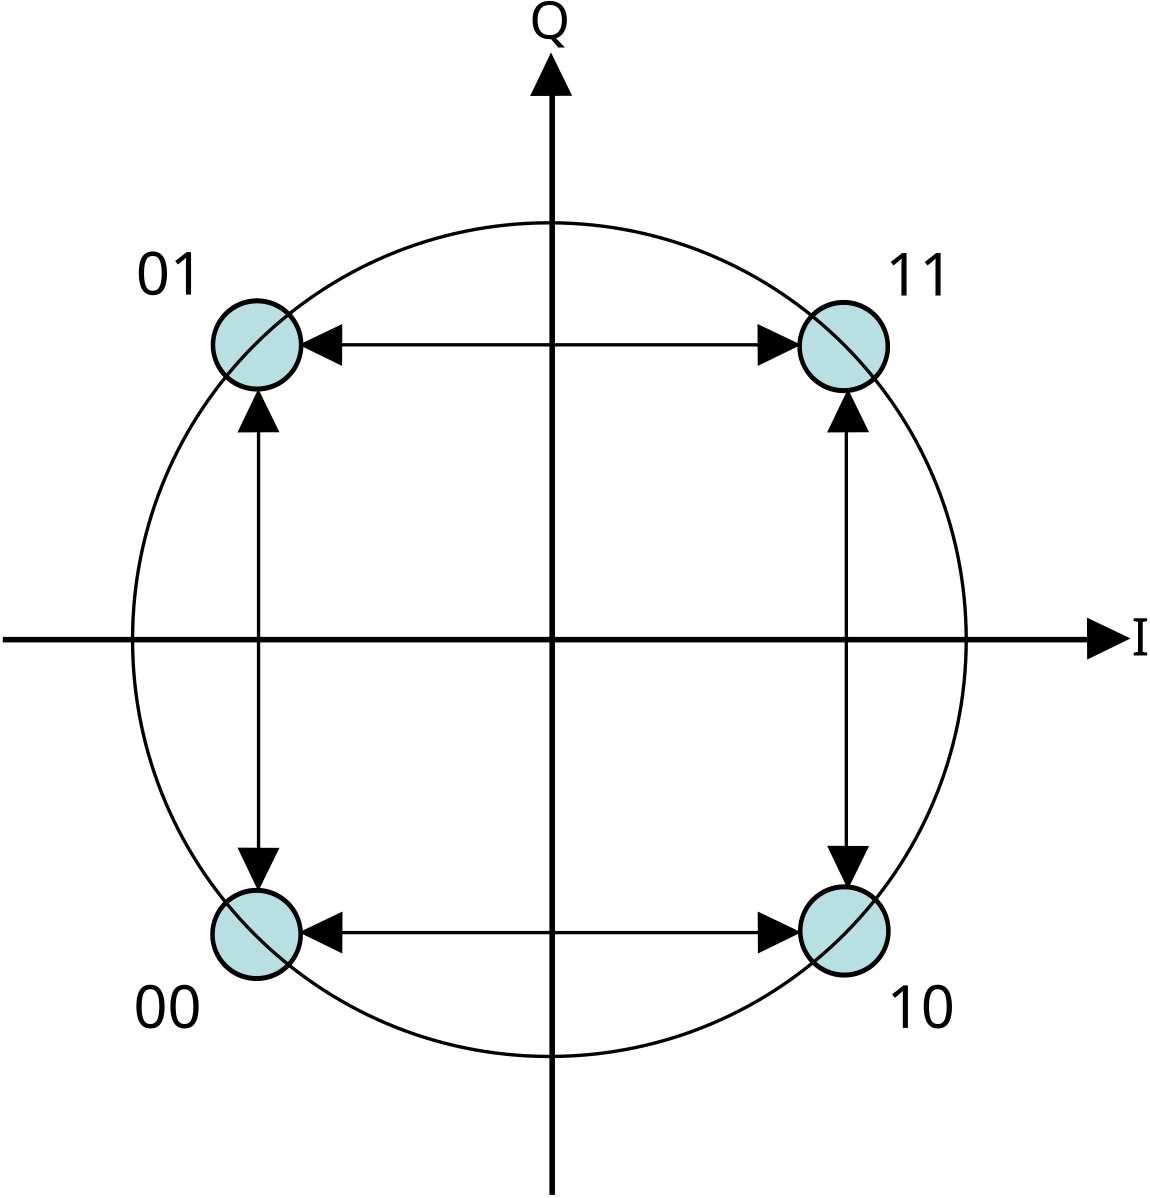
\includegraphics[width=0.4\linewidth]{./res/img/oqpsk_diagram.png}
  \caption{Diagramma per la costellazione OQPSK.}
  \label{fig:oqpsk-diagram}
\end{figure}

\subsection{Quadrature Amplitude Modulation (QAM)}
La modulazione \ac{QAM} trasmette segnali modulando le ampiezze di due onde portanti, utilizzando lo schema di modulazione digitale amplitude-shift keying (ASK) o lo schema di modulazione analogica amplitude modulation (AM). Le due onde portanti hanno la stessa frequenza e sono fuori fase tra loro di $90\degree$.
Il segnale trasmesso è creato sommando le due onde portanti tra di loro.
Al ricevitore, le due onde possono essere demodulate coerentemente grazie alla loro ortogonalità.
Nella \ac{QAM}, i punti della costellazione sono distribuiti in una griglia quadrata con spaziatura orizzontale e verticale uguale.

\begin{figure}[htbp]
  \centering
  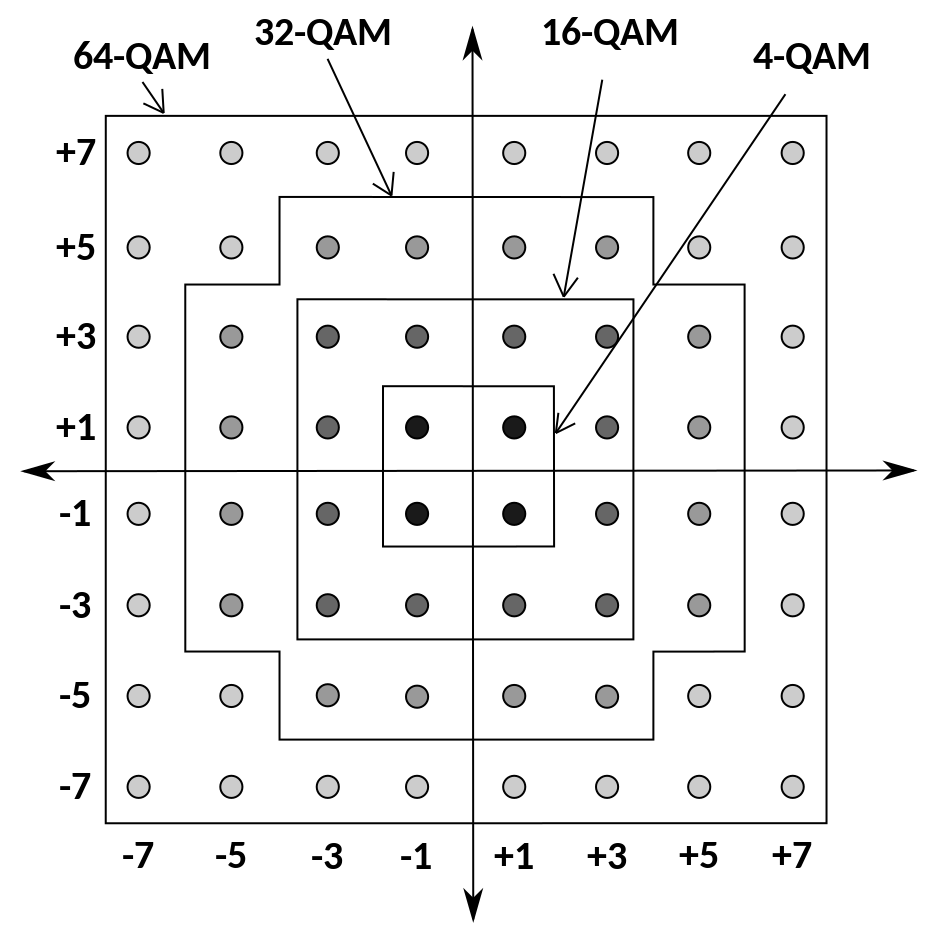
\includegraphics[width=0.6\linewidth]{./res/img/qam.png}
  \caption{Punti della costellazione per una 4-\ac{QAM}, 16-\ac{QAM}, 32-\ac{QAM} e 64-\ac{QAM} sovrapposti.}
  \label{fig:qam-diagram}
\end{figure}

Utilizzando una costellazione di ordine superiore è possibile trasmettere più bit per simbolo.
Però, se l'energia media della costellazione è la stessa, i punti devono essere più vicini tra di loro e quindi più suscettibili al rumore.
Questo risulta in un \ac{BER} più alto, e quindi costellazioni di ordine superiore possono fornire dati in modo meno affidabile rispetto alle costellazioni di ordine inferiore, con un'energia media costante.
Utilizzare \ac{QAM} di ordine più alto senza aumentare il \ac{BER} richiede un più alto \ac{SNR}, che si ottiene aumentando l'energia del segnale, riducendo il rumore, o facendo entrambe le cose.

Se sono richieste velocità di trasmissione dati superiori a quelle offerte da 8-\ac{PSK}, è più conveniente passare a \ac{QAM} poichè consente di ottenere una distanza maggiore tra i punti adiacenti nel piano complesso distribuendo i punti in modo più uniforme.
Il fattore che complica le cose è che i punti non sono più tutti alla stessa ampiezza e quindi il demodulatore deve identificare correttamente sia la fase che l'ampiezza, e non solo la fase.

\subsection{Orthogonal Frequency Division Multiplexing (OFDM)}
Orthogonal Frequency Division Multiplexing (\acs{OFDM}) è un metodo di codificare i dati digitali su più frequenze portanti.

\ac{OFDM} prende una sorgente di dati ad alta velocità e la divide in flussi più lenti che sono trasmessi simultaneamente attraverso un numero di sottoportanti ortogonali strettamente distanziate.
Le sottoportanti essendo ortogonali non interferiscono tra di loro, permettendo così un utilizzo molto efficiente della banda disponibile.
Al ricevitore, la sorgente di dati ad alta velocità è ricomposta usando l'algoritmo della trasformata veloce di Fourier (FFT).

\ac{OFDM} è in grado di far fronte a condizioni di canale difficili (come l'attenuazione delle alte freqeunze in un lungo filo di rame e l'interferenza in banda stretta) senza filtri complessi.
\ac{OFDM} può essere visto come l'utilizzo di molti segnali a banda stretta modulati lentamente piuttosto che di un unico segnale a banda larga modulato rapidamente, il che rende più semplice l'equalizzazione di canale (cioè la compensazione delle distorsioni ricevute dal segnale nel canale di comunicazione).
La bassa frequenza di simboli rende possibile l'utilizzo di un intervallo di guardia tra simboli, consentendo di eliminare l'interferenza intersimbolica (ISI) e di cancellare l'effetto dei cammini multipli e la dispersione temporale per ottenere un miglioramento del rapporto segnale rumore.

\subsubsection{Confronto della struttura del segnale con sistemi terrestri OFDM}
La struttura del segnale inviato da Starlink utilizza \ac{OFDM}, tuttavia, il progetto di Starlink differisce dai sistemi usati sulla terra per diversi aspetti chiave, che riflettono le caratteristiche uniche del canale di comunicazione spazio-terra.

\paragraph{Layout di canale} A differenza dei sistemi terresti dove la larghezza di banda e gli schemi di duplexing variano a livello regionale, Starlink impiega una struttura uguale in tutto il mondo per il downlink in banda Ku, con otto canali da 240 MHz separati da bande di guardia da 10 MHz.
Questa ampia banda di guardia consente di attivare più canali contemporaneamente all'interno di una cella di servizio e riduce al minimo le interferenze tra celle adiacenti.
In questo modo si riduce potenzialmente l'efficienza spettrale, ma si migliora l'affidabilità \cite{humphreys_signal_2023}.

\paragraph{Layout dei frame}
I frame inviati da Starlink, con un periodo di 1/750 secondi, hanno un layout che contiene un'alto numero di sequenze di sincronizzazione: la PSS, SSS, CM1SS e CSS.
Questa enfasi sulla sincronizzazione, superiore a quella dell'LTE e di altri sistemi terrestri, consente un'accurata equalizzazione del canale e stima dell'effetto Doppler, migliorando potenzialmente l'affidabilita della comunicazione e consentendo un doppio uso per il PNT (Positioning Navigation e Timing) \cite{humphreys_signal_2023}.

\paragraph{Sequenze di sincronizzazione}
L'utilizzo di sequenze di sincronizzazione multiple per frame, includendo il PSS m-sequence-based e la 4-\ac{QAM}-modulated SSS, lo distingue dai tradizionali sistemi terresti.
L'utilizzo di queste sequenze di sincronizzazione e la scelta di un numero moderato di sottoportanti semplificano l'elaborazione del segnale e garantiscono una sincronizzazione robusta anche in condizioni difficili \cite{humphreys_signal_2023}.

\paragraph{Efficienza e margini di design}
La struttura del segnale Starlink da priorità all'affidabilità.
L'efficiente occupazione dei simboli OFDM sfrutta il basso ritardo del canale \ac{LEO}-terra.
Le ampie bande di guardia e l'elevata occupazione dei frame, pur riducendo l'efficienza spettrale, migliorano la mitigazione delle interferenze e la precisione della sincronizzazione.
La scelta di un numero relativamente basso di sottoportanti (N = 1024) indica un design che prioritizza la robustezza piuttosto che massimizzare il throughput teorico \cite{humphreys_signal_2023}.

\section{Gestione del traffico}
Starlink gestisce il traffico dai terminali utenti alle ground station in un processo a due step.

\begin{figure}[htbp]
  \centering
  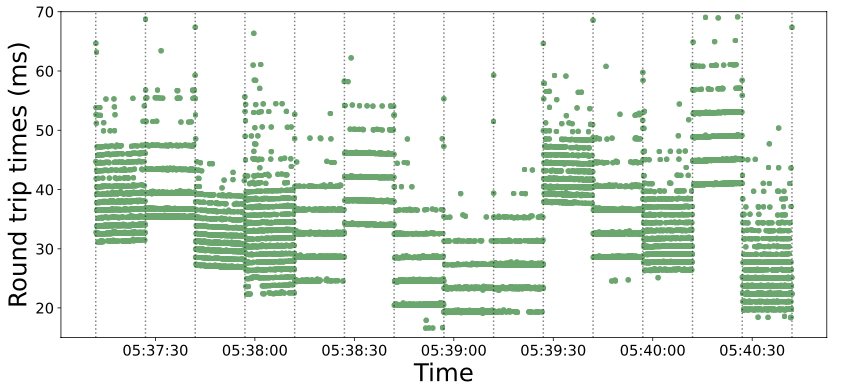
\includegraphics[width=0.8\linewidth]{./res/img/rtt_euterminal.png}
  \caption{\ac{RTT} misurato da un terminale in Europa \cite{tanveer_making_2023}.}
  \label{fig:rtt-euterminal}
\end{figure}

Come prima cosa un controller globale di rete alloca i satelliti ai terminali degli utenti basandosi su fattori quali il carico (inteso come banda del satellite occupata da altri utenti), le condizioni geospaziali (principalmente visibilità del satellite dal terminale utente e condizioni atmosferiche), e carica della batteria del satellite.
Da come si può vedere in figura \ref{fig:rtt-euterminal} i cambiamenti di latenza misurati avvengono ogni 15 secondi, e quindi le allocazioni vengono fatte ogni 15 secondi.

Come seconda cosa c'è un controller nel satellite, che pianifica i flussi dai terminali utente assegnati a un satellite specifico.
Questo si può notare dalla presenza di bande di latenza parallele negli intervalli di 15 secondi di allocazione dei terminali al satellite \cite{tanveer_making_2023} \cite{geoff_huston_transport_2024}.

Misure successive hanno rivelato che il servizio ha una velocità di download mediana di circa 120 Mbps in download, con picchi di 370 Mbps e minimi di 10 Mbps, e 15 Mbps di capacità in upload, con varianza tra i 5 Mbps e i 50 Mbps, come si può vedere in figura \ref{fig:starlink-performance} \cite{geoff_huston_transport_2024}.

\begin{figure}[htbp]
  \centering
  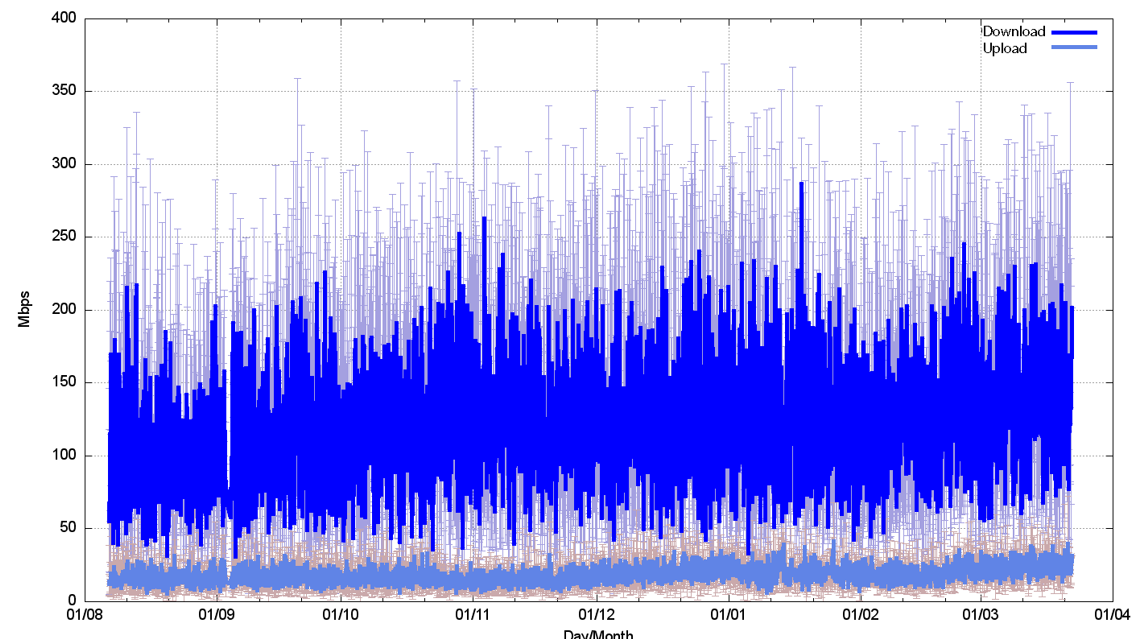
\includegraphics[width=0.8\linewidth]{./res/img/starlink_performance.png}
  \caption{Velocità della rete misurata da agosto 2023 a marzo 2024.}
  \label{fig:starlink-performance}
\end{figure}

Varianti tradizionali del \ac{TCP}, come Reno, faticano nell'ambiente delle comunicazioni satellitari, dato che utilizzano un incremento lineare della finestra di invio finché non ci sono perdite, e dimezzano la sua dimensione come risposta al packet loss.
Varianti moderne come CUBIC hanno prestazioni migliori grazie al Selective Acknowledgement (SACK), che permette di differenziare packet loss isolati da una congestione di rete, e utilizzano un tasso di incremento della dimensione della finestra variabile che tenta di stabilizzare il tasso di invio a un livello subito sotto la costruzione delle code di rete (che porta poi al packet loss).

In termini generali c'è un piccolo insieme di ipotesi comuni sulle caratteristiche del percorso di rete per questi algoritmi di controllo TCP.
\begin{itemize}
  \item Esiste una capacità massima stabile del percorso, dove il termine stabilità descrive una situazione in cui la capacità del percorso disponibile è relativamente costante su diversi intervalli di tempo di andata e ritorno (RTT).
  \item La quantità di jitter (variazione nel ritardo end-to-end) è bassa in proporzione all'RTT.
  \item Il tasso medio di perdita di pacchetti è basso. Nel caso di algoritmi di controllo TCP basati sulla perdita di pacchetti, la perdita di pacchetti è generalmente interpretata dall'algoritmo come un segno che i buffer della rete si sono riempiti e la perdita è un'indicazione di buffer overflow.
\end{itemize}

Ovviamente, come abbiamo notato, le prime due condizioni non valgono necessariamente per i percorsi end-to-end che includono un componente Starlink.
Anche il profilo di perdita è diverso.
Esiste la possibilità di una perdita di pacchetti indotta dalla congestione, come nel caso di qualsiasi mezzo a commutazione di pacchetto non sincrono, ma c'è una componente di perdita aggiuntiva che può verificarsi durante il trasferimento satellitare e un'ulteriore componente di perdita che può essere causata da altri problemi causati al segnale radio.

Il TCP in genere tende a reagire a tali ambienti utilizzando scelte conservative.

Anche il verificarsi di una perdita di pacchetti non basata sulla congestione può compromettere le prestazioni TCP. Convenzionalmente, la perdita indurrà il mittente a ridurre rapidamente la sua finestra di invio, sulla base del fatto che se questa perdita è causata da un overflow del buffer di rete, il mittente deve consentire a questi buffer di svuotarsi e quindi riprenderà a inviare a una velocità inferiore, il che dovrebbe ripristinare la coerenza del ciclo di controllo del feedback.

BBR, un algoritmo di controllo di congestione sviluppato da Google, ha dimostrato performance promettenti su Starlink mantenendo il tasso di invio anche durante la perdita di pacchetti.
L'algoritmo stima il prodotto banda-ritardo del percorso e aggiusta i tassi di invio basandosi sui cambiamenti di latenza.
Il problema di questo algoritmo è che la sua richiesta aggressiva di risorse può affamare le altre sessioni TCP \cite{geoff_huston_transport_2024}.

\subsection{Identificazioni delle allocazioni del satellite}
Per studiare l'algoritmo di scheduling, i ricercatori hanno dovuto identificare a quale satellite si connettevano i terminali utente.
L'applicazione per telefono di Starlink non fornisce più informazioni sul satellite a cui si connette il proprio terminale.
Si cerca di correlare le posizioni conosciute pubblicamente dei satelliti Starlink con le osservazioni delle mappe di ostruzione registrate in ciascun terminale.

\paragraph{Mappe di ostruzione}
Le mappe di ostruzione sono immagini bidimensionali che segnano la traiettoria di satelliti che hanno recentemente servito il terminale utente.
Queste immagini sono usate per creare una mappa tridimensionale che viene poi resa disponibile agli utenti, per aiutarli a identificare la qualità della posizione dove è stato disposto il loro terminale, evidenziando ostruzioni fisiche tra il loro terminale e il satellite.
La figura \ref{fig:obstruction-maps} mostra un esempio di questa mappa dall'applicazione di Starlink nella figura a destra.
Le figure al centro e a sinistra invece mostrano esempi di queste mappe per slot di 15 secondi usando \verb|starlink-grpc-tools|\cite{sparky8512_starlink-grpc-tools_nodate}.

\begin{figure}[htbp]
  \centering
  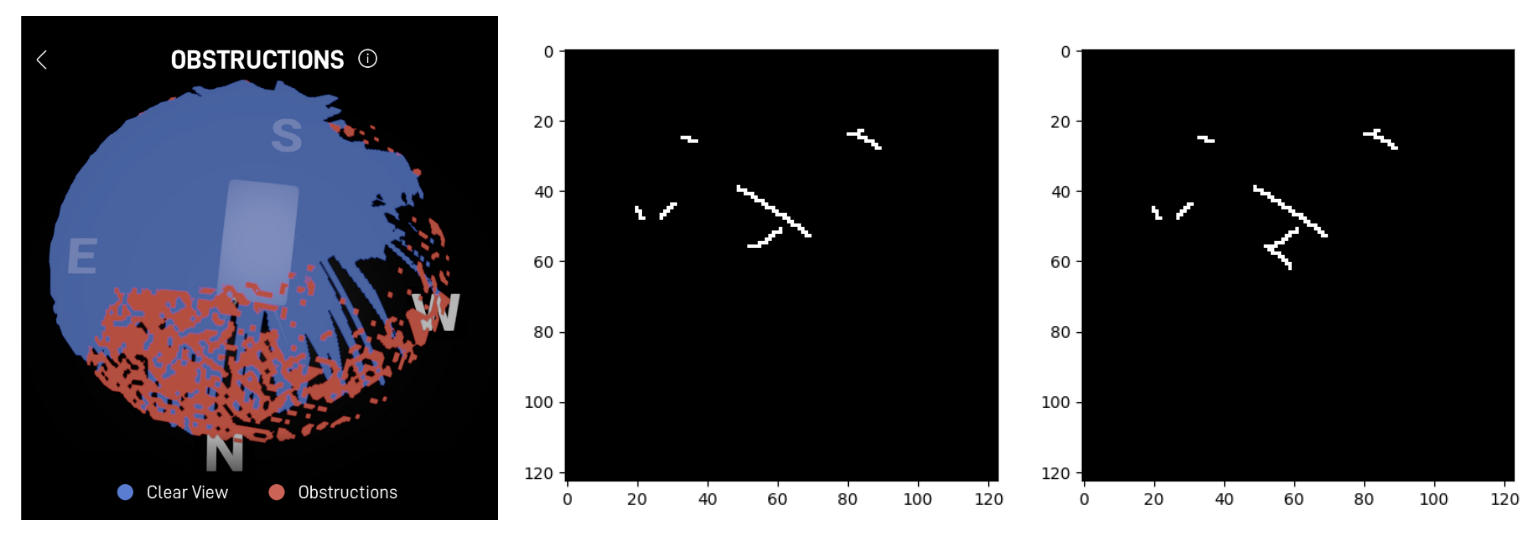
\includegraphics[width=0.7\linewidth]{./res/img/obstruction_maps.png}
  \caption{Mappa di ostruzione ottenuta dall'app di Starlink (sinistra) e da gRPC \cite{sparky8512_starlink-grpc-tools_nodate}\cite{tanveer_making_2023}.}
  \label{fig:obstruction-maps}
\end{figure}

Allineando le mappe 2D di \verb|starlink-grpc-tools| con le mappe 3D ottenute dall'applicazione di Starlink e isolando la traiettoria del satellite connesso durante lo slot di 15 secondi si riesce a identificare il satellite che serve il terminale utente.

\subsection{Caratteristiche e preferenze dello scheduler globale}
Le analisi dei satelliti allocati hanno rivelato diverse preferenze dello scheduler globale. Si possono individuare tre fattori determinanti per la scelta:
\begin{itemize}
  \item Posizione del satellite: lo scheduler preferisce satelliti con angoli di elevazione più alti, con la mediana dei satelliti selezionati a 22.9 gradi più alta di quelli non selezionati \cite{tanveer_making_2023}.
  Lo scheduler ha anche una preferenza per i satelliti a nord del terminale utente. Questo probabilmente è dovuto alla zona di esclusione dell'International Telecommunication Union per le orbite geostazionarie e considerazioni di efficienza energetica, dato che i satelliti con un angolo di elevazione più alto hanno bisogno di meno energia per la comunicazione \cite{tanveer_making_2023}.
  \item Data di lancio del satellite: lo scheduler dà priorità ai satelliti più nuovi, infatti la probabilità che un satellite sia selezionato aumenta all'aumentare della sua data di lancio. Questa preferenza potrebbe essere legata al mantenimento di una copertura stabile della costellazione, dato che i satelliti più vecchi stanno raggiungendo la fine del loro ciclo di vita.
  \item Stato di illuminazione: lo scheduler favorisce i satelliti illuminati dal sole, scegliendoli il 72.3\% delle volte quando sono disponibili sia satelliti illuminati che non. I satelliti non illuminati sono selezionati solo quando rappresentano almeno il 35\% dei satelliti disponibili. La scelta sembra comunque guidata dal fatto che il loro angolo di elevazione sia maggiore di quelli illuminati, probabilmente per risparmiare energia \cite{tanveer_making_2023}.
\end{itemize}


    %!TEX root = ../main.tex

\chapter{Conclusioni e sviluppi futuri}
\label{chp:conclusions}

In questo studio si è analizzata l'architettura di rete di Starlink attraverso le informazioni pubblicamente disponibili, la maggior parte delle quali è stata reperita tramite ingegnerizzazione inversa dell' antenna e della rete, e l'analisi delle informazioni pubblicamente disponibili dalle archiviazioni fatte da SpaceX presso la Federal Communications Commission (FCC), fatte per ottenere i permessi per lo sviluppo della costellazione di satelliti \cite{jonathan_mcdowell_section_nodate}.

Starlink è utilizzato nella guerra Russo-Ucraina, ruolo per il quale è stato incaricato dal dipartimento della difesa degli Stati Uniti \cite{amanda_macias_pentagon_2023}.

Gli astronomi hanno espresso preoccupazione per l'effetto che la costellazione potrebbe avere sull'astronomia terrestre e per il modo in cui i satelliti contribuiranno a un ambiente orbitale già congestionato \cite{nadia_drake_will_2019}.
SpaceX ha cercato di mitigare le preoccupazioni relative alle interferenze astronomiche con misure volte a ridurre la luminosità dei satelliti durante il funzionamento \cite{starlink_brightness_nodate}.

Il prossimo step importante nel progetto di Starlink ora sono i satelliti "V2 Mini", che hanno una capacità di connessione di 4 volte maggiore rispetto alla versione 1.5.
I satelliti V2 Mini sono uno step intermedio tra il design originale e un design ancora più grande che SpaceX progetta di inserire nel razzo Starship.
Starship ha quasi 10 volte la capacità di carico del payload di un razzo Falcon 9, che viene attualmente utilizzato per lanciare i satelliti,  oltre ad avere più volume per il trasporto.
I satelliti V2 Mini saranno in grado di trasmettere segnale direttamente ai cellulari, avranno antenne Phased Array più potenti e introdurrano l'E-band (il range di frequenze radio che va dai 60 GHz ai 90 GHz nello spettro elettromagnetico) per la rete di ritorno (quella che va dai satelliti alle ground station).
I satelliti sono dotati di propulsori a effetto Hall che consentono loro di innalzare l'orbita, di stazionare, e di deorbitare al termine della loro vita.
Questi propulsori utilizzano Argon, un gas più economico del carburante Krypton, utilizzato nella prima generazione di satelliti.
Sono inoltre progettati per evitare autonomamente e senza problemi le collisisoni con altri satelliti sulla base dei dati di tracciamento.
Ciascun satellite V2 Mini pesa circa 800 kg, che lo rende quasi tre volte più pesante dei satelliti della prima generazione \cite{starlink_secon_nodate}.

\begin{figure}[htbp]
  \centering
  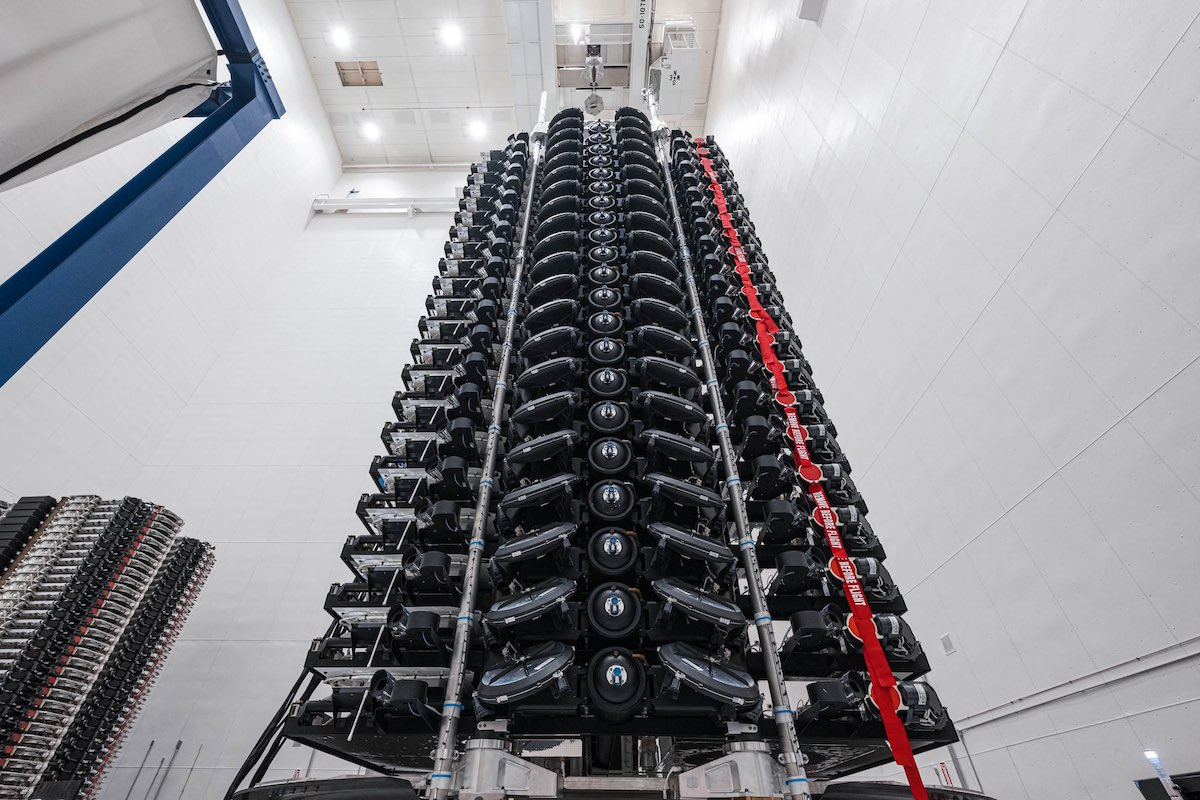
\includegraphics[width=0.8\linewidth]{./res/img/satellite_v2mini.jpg}
  \caption{Primo lotto dei satelliti "V2 Mini" pronto per il lancio in un razzo Falcon 9 da Cape Canaveral.}
  \label{fig:satellite_v2mini}
\end{figure}

Nel novembre 2024 SpaceX ha proposto una nuova iniziativa chiamata "Marslink", una versione adatta per Marte del suo sistema satellitare Starlink, per fornire servizi di trasmissione dati ad alta velocità tra Marte e la Terra. 
Il progetto, presentato a una riunione del NASA Mars Exploration Program Analysis Group, delinea l'utilizzo di satelliti in orbita attorno a Marte per garantire comunicazioni e supporto continui per le missioni di esplorazione.
Marslink mira a superare la velocità di trasmissione dati richiesta dalla NASA di 4 Mbps.
Questo sistema sfrutterebbe la tecnologica di comunicazione laser, consentendo il trasferimento di dati a lunga distanza attraverso le 1.5 unità astronomiche che separano Marte dal Sole \cite{michael_kan_spacex_2024}.

Starlink ha raggiunto 4 milioni di clienti a settembre 2024 \cite{starlink_starlink_nodate}.

\begin{figure}[htbp]
  \centering
  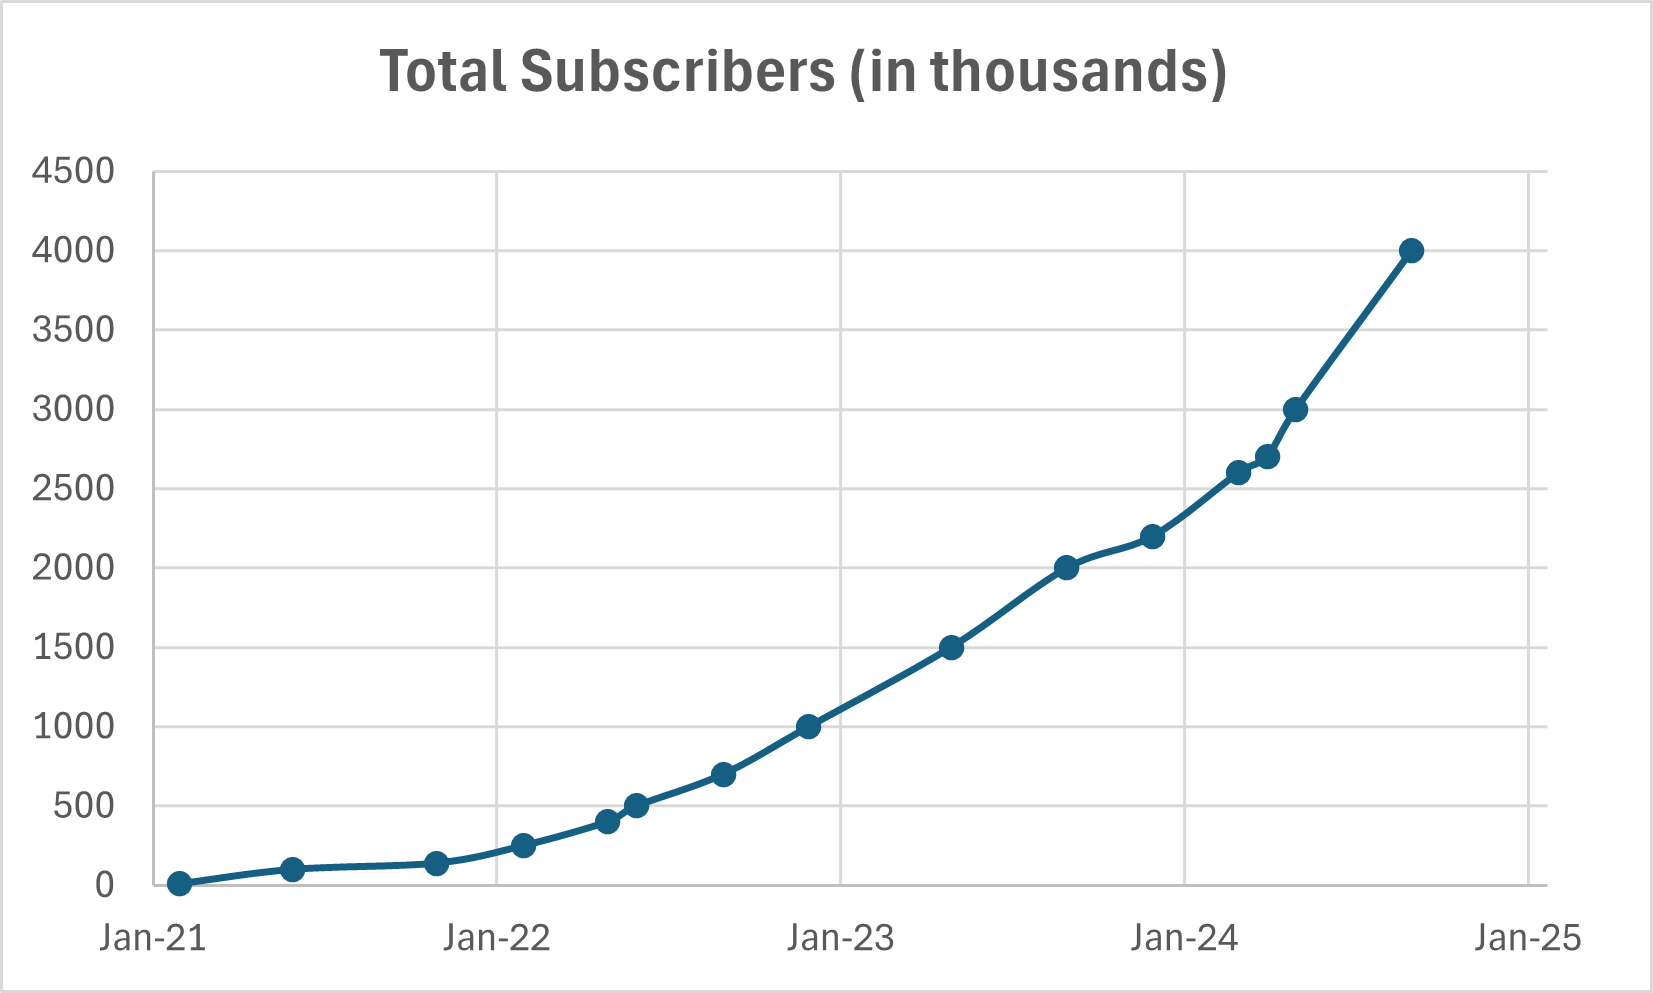
\includegraphics[width=0.8\linewidth]{./res/img/chart_subs.png}
  \caption{Numero di utenti di Starlink.}
  \label{fig:chart-subs}
\end{figure}


    
    % Bibliography, appendix, acknowledges, etc...
    \backmatter
\end{document}